%%%%%%%%%%%%%%%%%%%%%%%%%%%%%%%%%%%%%%%%%
% Masters/Doctoral Thesis 
% LaTeX Template
% Version 2.4 (22/11/16)
%
% This template has been downloaded from:
% http://www.LaTeXTemplates.com
%
% Version 2.x major modifications by:
% Vel (vel@latextemplates.com)
%
% This template is based on a template by:
% Steve Gunn (http://users.ecs.soton.ac.uk/srg/softwaretools/document/templates/)
% Sunil Patel (http://www.sunilpatel.co.uk/thesis-template/)
%
% Template license:
% CC BY-NC-SA 3.0 (http://creativecommons.org/licenses/by-nc-sa/3.0/)
%
%%%%%%%%%%%%%%%%%%%%%%%%%%%%%%%%%%%%%%%%%

%----------------------------------------------------------------------------------------
%	PACKAGES AND OTHER DOCUMENT CONFIGURATIONS
%----------------------------------------------------------------------------------------

\documentclass[
11pt, % The default document font size, options: 10pt, 11pt, 12pt
%oneside, % Two side (alternating margins) for binding by default, uncomment to switch to one side
english, % ngerman for German
singlespacing, % Single line spacing, alternatives: onehalfspacing or doublespacing
%draft, % Uncomment to enable draft mode (no pictures, no links, overfull hboxes indicated)
%nolistspacing, % If the document is onehalfspacing or doublespacing, uncomment this to set spacing in lists to single
%liststotoc, % Uncomment to add the list of figures/tables/etc to the table of contents
%toctotoc, % Uncomment to add the main table of contents to the table of contents
%parskip, % Uncomment to add space between paragraphs
%nohyperref, % Uncomment to not load the hyperref package
headsepline, % Uncomment to get a line under the header
%chapterinoneline, % Uncomment to place the chapter title next to the number on one line
%consistentlayout, % Uncomment to change the layout of the declaration, abstract and acknowledgements pages to match the default layout
]{MastersDoctoralThesis} % The class file specifying the document structure

\usepackage[utf8]{inputenc} % Required for inputting international characters
\usepackage[T1]{fontenc} % Output font encoding for international characters

\usepackage{palatino} % Use the Palatino font by default

\usepackage[backend=bibtex,style=authoryear]{biblatex} % Use the bibtex backend with the authoryear citation style (which resembles APA)

%% temp fix for bibtex
\makeatletter
\def\blx@maxline{77}
\makeatother

\usepackage{amssymb, amsmath}
\usepackage{epsfig}
\usepackage{array}
\usepackage{ifthen}
\usepackage{color}
\usepackage{graphicx}
\usepackage{mathtools}
\usepackage{multirow}
\usepackage{xcolor}
\usepackage{chngcntr}
\usepackage{apptools}
\usepackage{tikz}
\usetikzlibrary{shapes,arrows}

\addbibresource{example.bib} % The filename of the bibliography

\usepackage[autostyle=true]{csquotes} % Required to generate language-dependent quotes in the bibliography

%----------------------------------------------------------------------------------------
%	MARGIN SETTINGS
%----------------------------------------------------------------------------------------

\geometry{
	paper=a4paper, % Change to letterpaper for US letter
	inner=2.5cm, % Inner margin
	outer=3.8cm, % Outer margin
	bindingoffset=.5cm, % Binding offset
	top=1.5cm, % Top margin
	bottom=1.5cm, % Bottom margin
	%showframe, % Uncomment to show how the type block is set on the page
}

%----------------------------------------------------------------------------------------
%	THESIS INFORMATION
%----------------------------------------------------------------------------------------

\thesistitle{Randomized classification: theory and applications} % Your thesis title, this is used in the title and abstract, print it elsewhere with \ttitle
\supervisor{Dr. Trevor \textsc{Hastie} and Dr. Jonathan \textsc{Taylor}} % Your supervisor's name, this is used in the title page, print it elsewhere with \supname
\examiner{} % Your examiner's name, this is not currently used anywhere in the template, print it elsewhere with \examname
\degree{Doctor of Philosophy} % Your degree name, this is used in the title page and abstract, print it elsewhere with \degreename
\author{Charles \textsc{Zheng}} % Your name, this is used in the title page and abstract, print it elsewhere with \authorname
\addresses{} % Your address, this is not currently used anywhere in the template, print it elsewhere with \addressname

\subject{Statistics} % Your subject area, this is not currently used anywhere in the template, print it elsewhere with \subjectname
\keywords{} % Keywords for your thesis, this is not currently used anywhere in the template, print it elsewhere with \keywordnames
\university{\href{http://www.stanford.edu}{Stanford University}} % Your university's name and URL, this is used in the title page and abstract, print it elsewhere with \univname
\department{\href{http://statweb.stanford.edu}{Department of Statistics}} % Your department's name and URL, this is used in the title page and abstract, print it elsewhere with \deptname
\group{\href{http://researchgroup.university.com}{Research Group Name}} % Your research group's name and URL, this is used in the title page, print it elsewhere with \groupname
\faculty{\href{http://faculty.university.com}{Faculty Name}} % Your faculty's name and URL, this is used in the title page and abstract, print it elsewhere with \facname

\AtBeginDocument{
\hypersetup{pdftitle=\ttitle} % Set the PDF's title to your title
\hypersetup{pdfauthor=\authorname} % Set the PDF's author to your name
\hypersetup{pdfkeywords=\keywordnames} % Set the PDF's keywords to your keywords
}


\newcommand{\tr}{\text{tr}}
\newcommand{\E}{\textbf{E}}
\newcommand{\diag}{\text{diag}}
\newcommand{\argmax}{\text{argmax}}
\newcommand{\Cov}{\text{Cov}}
\newcommand{\Var}{\text{Var}}
\newcommand{\argmin}{\text{argmin}}
\newcommand{\Vol}{\text{Vol}}
\newcommand{\comm}[1]{}
\newcommand{\indep}{\rotatebox[origin=c]{90}{$\models$}}
\newcommand{\Cor}{\text{Cor}}
\newcommand{\bx}{\boldsymbol{x}}
\newcommand{\by}{\boldsymbol{y}}
\newcommand{\bX}{\boldsymbol{X}}
\newcommand{\bY}{\boldsymbol{Y}}
\newcommand{\bS}{\boldsymbol{S}}
\newcommand{\bu}{\boldsymbol{u}}
\newcommand{\bv}{\boldsymbol{v}}
\newcommand{\bU}{\boldsymbol{U}}
\newcommand{\bV}{\boldsymbol{V}}
\newcommand{\bB}{\boldsymbol{B}}
\newcommand{\bepsilon}{\boldsymbol{\epsilon}}
\newcommand{\bH}{\boldsymbol{H}}

\newtheorem{theorem}{Theorem}[section]
\newtheorem{proposition}{Proposition}[section]
\newtheorem{corollary}{Corollary}[theorem]
\newtheorem{lemma}{Lemma}[section]
\newtheorem{definition}{Definition}[section]

\begin{document}

\frontmatter % Use roman page numbering style (i, ii, iii, iv...) for the pre-content pages

\pagestyle{plain} % Default to the plain heading style until the thesis style is called for the body content

%----------------------------------------------------------------------------------------
%	TITLE PAGE
%----------------------------------------------------------------------------------------

\begin{titlepage}
\begin{center}

\vspace*{.06\textheight}
{\scshape\LARGE \univname\par}\vspace{1.5cm} % University name
\textsc{\Large Doctoral Thesis}\\[0.5cm] % Thesis type

\HRule \\[0.4cm] % Horizontal line
{\huge \bfseries \ttitle\par}\vspace{0.4cm} % Thesis title
\HRule \\[1.5cm] % Horizontal line
 
\begin{minipage}[t]{0.4\textwidth}
\begin{flushleft} \large
\emph{Author:}\\
\href{http://www.johnsmith.com}{\authorname} % Author name - remove the \href bracket to remove the link
\end{flushleft}
\end{minipage}
\begin{minipage}[t]{0.4\textwidth}
\begin{flushright} \large
\emph{Supervisor:} \\
\href{http://www.jamessmith.com}{\supname} % Supervisor name - remove the \href bracket to remove the link  
\end{flushright}
\end{minipage}\\[3cm]
 
\vfill

\large \textit{A thesis submitted in fulfillment of the requirements\\ for the degree of \degreename}\\[0.3cm] % University requirement text
\textit{in the}\\[0.4cm]
%\groupname\\
\deptname\\[2cm] % Research group name and department name
 
\vfill

{\large \today}\\[4cm] % Date
%\includegraphics{Logo} % University/department logo - uncomment to place it
 
\vfill
\end{center}
\end{titlepage}

%----------------------------------------------------------------------------------------
%	DECLARATION PAGE
%----------------------------------------------------------------------------------------
\iffalse

\begin{declaration}
\addchaptertocentry{\authorshipname} % Add the declaration to the table of contents
\noindent I, \authorname, declare that this thesis titled, \enquote{\ttitle} and the work presented in it are my own. I confirm that:

\begin{itemize} 
\item This work was done wholly or mainly while in candidature for a research degree at this University.
\item Where any part of this thesis has previously been submitted for a degree or any other qualification at this University or any other institution, this has been clearly stated.
\item Where I have consulted the published work of others, this is always clearly attributed.
\item Where I have quoted from the work of others, the source is always given. With the exception of such quotations, this thesis is entirely my own work.
\item I have acknowledged all main sources of help.
\item Where the thesis is based on work done by myself jointly with others, I have made clear exactly what was done by others and what I have contributed myself.\\
\end{itemize}
 
\noindent Signed:\\
\rule[0.5em]{25em}{0.5pt} % This prints a line for the signature
 
\noindent Date:\\
\rule[0.5em]{25em}{0.5pt} % This prints a line to write the date
\end{declaration}

\cleardoublepage

\fi
%----------------------------------------------------------------------------------------
%	QUOTATION PAGE
%----------------------------------------------------------------------------------------

%\vspace*{0.2\textheight}

%\noindent\enquote{\itshape Thanks to my solid academic training, today I can write hundreds of words on virtually any topic without possessing a shred of information, which is how I got a good job in journalism.}\bigbreak

%\hfill Dave Barry

%----------------------------------------------------------------------------------------
%	ABSTRACT PAGE
%----------------------------------------------------------------------------------------
\iffalse

\begin{abstract}
\addchaptertocentry{\abstractname} % Add the abstract to the table of contents
The Thesis Abstract is written here (and usually kept to just this page). The page is kept centered vertically so can expand into the blank space above the title too\ldots
\end{abstract}

\fi
%----------------------------------------------------------------------------------------
%	ACKNOWLEDGEMENTS
%----------------------------------------------------------------------------------------
\iffalse

\begin{acknowledgements}
\addchaptertocentry{\acknowledgementname} % Add the acknowledgements to the table of contents
The acknowledgments and the people to thank go here, don't forget to include your project advisor\ldots
\end{acknowledgements}

\fi
%----------------------------------------------------------------------------------------
%	LIST OF CONTENTS/FIGURES/TABLES PAGES
%----------------------------------------------------------------------------------------

\tableofcontents % Prints the main table of contents

%\listoffigures % Prints the list of figures

%\listoftables % Prints the list of tables

%----------------------------------------------------------------------------------------
%	ABBREVIATIONS
%----------------------------------------------------------------------------------------

%\begin{abbreviations}{ll} % Include a list of abbreviations (a table of two columns)
%\textbf{LAH} & \textbf{L}ist \textbf{A}bbreviations \textbf{H}ere\\
%\textbf{WSF} & \textbf{W}hat (it) \textbf{S}tands \textbf{F}or\\
%\end{abbreviations}

%----------------------------------------------------------------------------------------
%	PHYSICAL CONSTANTS/OTHER DEFINITIONS
%----------------------------------------------------------------------------------------

%\begin{constants}{lr@{${}={}$}l} % The list of physical constants is a three column table
%Speed of Light & $c_{0}$ & \SI{2.99792458e8}{\meter\per\second} (exact)\\
%\end{constants}

%----------------------------------------------------------------------------------------
%	SYMBOLS
%----------------------------------------------------------------------------------------

%\begin{symbols}{lll} % Include a list of Symbols (a three column table)
%$a$ & distance & \si{\meter} \\
%$P$ & power & \si{\watt} (\si{\joule\per\second}) \\
%\addlinespace % Gap to separate the Roman symbols from the Greek
%$\omega$ & angular frequency & \si{\radian} \\
%\end{symbols}

%----------------------------------------------------------------------------------------
%	DEDICATION
%----------------------------------------------------------------------------------------

%\dedicatory{For/Dedicated to/To my\ldots} 

%----------------------------------------------------------------------------------------
%	THESIS CONTENT - CHAPTERS
%----------------------------------------------------------------------------------------

\mainmatter % Begin numeric (1,2,3...) page numbering

\pagestyle{thesis} % Return the page headers back to the "thesis" style

% Include the chapters of the thesis as separate files from the Chapters folder
% Uncomment the lines as you write the chapters

% Chapter 1

\chapter{Introduction} % Main chapter title

\label{Chapter1} % For referencing the chapter elsewhere, use \ref{Chapter1} 

%----------------------------------------------------------------------------------------

% Define some commands to keep the formatting separated from the content 
\newcommand{\keyword}[1]{\textbf{#1}}
\newcommand{\tabhead}[1]{\textbf{#1}}
\newcommand{\code}[1]{\texttt{#1}}
\newcommand{\file}[1]{\texttt{\bfseries#1}}
\newcommand{\option}[1]{\texttt{\itshape#1}}

%----------------------------------------------------------------------------------------


\section{Recognition tasks}

The study of human intelligence, and the study of artificial
intelligence, form two major intertwining areas of modern research.
The attempt to algorithmically mimic or exceed human perceptual and
cognitive capabilities not only advances the application of artificial
intelligence for industrial applications, but also sheds light on the
nature of biological intelligence, and the nature of intelligence in
general.  One of the key capabilities of an intelligent system,
natural or artificial, is the ability to recognize objects, agents,
and signs in the environment based on input data.  Human brains have a
remarkable ability to recognize objects, faces, spoken syllables and
words, and written symbols or words, and this recognition ability is
essential for everyday life.  While researchers in artificial
intelligence have attempted to meet human benchmarks for these
classical recognition tasks for the last X decades, only very recent
advances in machine learning, such as deep neural networks, have
allowed algorithmic recognition algorithms to approach or exceed human
performance [CITE].

Within the statistics and machine learning literature, the usual
formalism for studying a recognition task is to pose it as a
\emph{multi-class classification} problem.  One delineates a finite
set of distinct entities which are to be recognized and distinguished,
which is the \emph{label set} $\mathcal{Y}$.  The input data is
assumed to take the form of a finite-dimensional real \emph{feature
  vector} $X \in \mathbb{R}^p$.  Each input instance is associated
with exactly one true label $Y \in \mathcal{Y}$.  The solution to the
classification problem takes the form of an algorithmically
implemented \emph{classification rule} $h$ that maps vectors $X$ to
predicted labels $\hat{Y} \in \mathcal{Y}$.  The classification rule
can be constructed in a data-dependent way: that is, one collects a
number of labelled \emph{training observations} $(X_1, Y_1)$ which is
used to inform the construction of the classification rule $h$.  The
success of the classification rule $h$ is measured by the \emph{expected loss} or \emph{risk},
which in the case of zero-one loss takes the form
\[
\text{Risk}(h) = \Pr[h(X) \neq Y],
\]
where the probability is defined with reference to the unknown
population joint distribution of $(X, Y)$.  
%A common approach for
%constructing a classifier $h$ is \emph{empirical risk minimization} [CITE],
%which constructs $h$ by minimizing the objective function
%\[
%\text{EmpiricalRisk}_{h \in \mathcal{H}}(h) = \frac{1}{n} \sum_{i=1}^n I(h(X) \neq Y)
%\]
%where $\mathcal{H}$ is some pre-specified function class.

However, a limitation of the usual multi-class classification
framework for studying recognition problems is the assumption that the
label set $\mathcal{Y}$ is finite and known in advance.  When
considering human recognition capabilities, it is clear that this is
not the case.  Our ability to recognize faces is not limited to some
pre-defined, fixed set of faces; same with our ability to recognize
objects in the environment.  Humans learn to recognize novel faces and
objects on a daily basis.  And, if artificial intelligence is to fully
match the human capability for recognition, it must also possess the
ability to add new categories of entities to its label set over time;
however, at present, there currently exists a void in the machine
learning literature on the subject of the online learning of new
classes in the data [CITE].

The central theme of this thesis is the study of \emph{randomized
  classification}, which can be motivated as an extension of the
classical multi-class classification framework to accommodate the
possibility of growing or infinite label sets $\mathcal{Y}$. The basic
approach taken is to assume an infinite or even continuous label space
$\mathcal{Y}$, and then to study the problem of classification on
finite label sets $S$ which are randomly sampled from $\mathcal{Y}.$
This, therefore defines a \emph{randomized classification} problem
where the label set is finite but may vary from instance to instance.
One can then proceed to answer questions about the variability of the
performance due to randomness in the labels, or how performance
changes depending on the size of the random label set.

An additional set of applications of the randomized classification
framework lies in its connection to information theory.  Randomized
classification is the natural analogue of the \emph{random code}
models first studied by Claude Shannon.  Furthermore, it becomes
possible to prove extensions of Fano's inequality to the case of
continuous $X$ and $Y$ by means of randomized classification.
Therefore, randomized classification can be used as a means of
inferring mutual information.

The rest of the thesis is organized as follows.  The remaining
sections in this chapter deal with background material on supervised
learning and information theory, as well as the application of both to
neuroscience, which forms a major motivation for the current work.
Chapter 2 introduces the concept of randomized classification, and
also establishes some variability bounds which will be used later in
the development of inference procedures.  Chapter 3 studies the
dependence of classification accuracy on the label set size in
randomized classification, and a practical method for predicting the
accuracy-versus-label set size curve from real data.  Chapter 4 and 5
deal with the applications of randomized classification to the
estimation of mutual information in continuous data: chapter 4 derives
a lower confidence bound for mutual information under very weak
assumptions, while chapter 5 works within an asymptotic
high-dimensional framework which leads to a more powerful but less
robust estimator estimate of mutual information.

\section{Information and Discrimination}

In studying the problem of recognition, we make use of two closely
related frameworks: firstly, the multi-class classification framework
from the statistics and machine learning literature, and secondly, the
concepts of information theory.  From a broader perspective, this is
hardly unusual, since concepts such as entropy, divergence, and mutual
information are commonly applied in theoretical statistics and machine
learning.  Furthermore, information theory, theoretical statistics,
and machine learning are based on the same foundation:
measure-theoretic probability theory; one could even say that all
three disciplines are subfields of applied probability.  However,
while the three sub-fields may appear very similar from a mathematical
perspective, some differences arise if we examine the kinds of
intuitions and assumptions that are characteristic of the literature
in each area.

A common problem to all three subfields is the inference of some
unobserved quantity on the basis of observed quantities.  In classical
statistics, the problem is to infer an unknown parameter; in
supervised learning, the problem is to predict an unobserved label or
response $Y$; in information theory, the problem is to decode a noisy
message.  Next, the metric for quantifying achievable performance
differs between the three disciplines.  In classical statistics, one
is concerned with the variance of the estimated parameter, or
equivalently, the Fisher information.  In machine learning, one seeks
to minimize (in expectation) a \emph{loss} function which measures the
discrepancy between the prediction and the truth.  In information
theory, one can measure the quality of the noisy channel (and
therefore, the resulting achievable accuracy) through the \emph{mutual
  information} $I(X; Y)$ between the sender's encoded message $X$ and
the reciever's recieved message $Y$.  If we specialize within machine
learning to the study of classification, then we are concerned with
accurate \emph{discrimination} of the input $X$ according to labels
$Y$.  Similarly, if we specialize to the problem of hypothesis testing
within statistics, the the problem is again to \emph{discriminate}
between two (or more) different hypotheses regarding the
data-geenrating mechanism.

%% have to reorder the next para, 
The concepts of \emph{information} and \emph{discrimination} are quite
distinct from an intuitive standpoint; however, they are linked at a
fundamental level.  This link can be seen throughout statistics and
machine learning, and in the way we think about statistical problems.
A statistical hypothesis test is \emph{informative} because it
provides evidence that the data behaves according to a certain
hypothesis rather than another.  %% slightly redundant with prev para.
In information theory, even if the reciever cannot conclusively
determine the sender's message from the observed signal, the signal
still contains \emph{information} if it contains some evidence that
favors one set of possible messages over another.  The formalism of
measure-theoretic probability theory provides yet another example of
the conceptual link between information and
discrimination\footnote{Supposing $\Omega$ is a probability space
  defined with respect to a $\sigma$-algebra $\mathcal{F}$, we can
  represent our state of knowledge with a filtration (or
  sub-$\sigma$-algebra) $\mathcal{F}' \subseteq \mathcal{F}$.
  Complete knowledge (zero uncertainty) is represented by the full
  $\sigma$-algebra: that is, $\mathcal{F}' = \mathcal{F}$.  Partial
  knowledge is represented by a coarser filtration, $\mathcal{F}
  \subset \mathcal{F}'$.  The filtration, of course, indicates that
  our knowledge is sufficient to \emph{discriminate} the outcome space
  $\Omega$ into a number of finitely or infinitely many categories.
  The more information we have, (or, the closer we come to complete
  knowledge of the outcome), the more finely we can discriminate the
  realized outcomes given by $\omega \in \Omega$.}.

%% the purpose of this paragraph is to make the link between discrimination and information
%% this para needs work after being moved
Either natural or artificially intelligence recognition systems must
rely on input data that is \emph{informative} of the optimal response
if they are to achieve reasonable discriminative accuracy.  In natural
environments, mammals rely on a combination of visual, auditory, and
tactile cues to recognize potential threats in the environment.
Mammalian brains integrate all of this sensory information in order to
make more rapid and reliable decisions.  Generally, increased
diversity and quality of the available sources of information will
lead to more accurate recognition (say, of possible environmental
threats.)

This link between the information content of the input and the
achievable discrimination accuracy was first quantified by Claude
Shannon via the concept of \emph{mutual information.}  The mutual
information $I(X; Y)$ quantifies the information content that an input
$X$ holds abut a target of interest, $Y$.  For instance, in the case
of facial identification, the discrimination target $Y$ is a label
corresponding to the identity of the person, and $X$ is an image of
the individual's face.  An image corrupted by noise holds less
information, and correspondingly leads to lower classification
accuracies.

The discrmination problem that Shannon studied--the
\emph{noisy-channel decoding problem}, is extremely similar to the
multi-class classification problem, but also features some important
differences.  A side-by side comparison between the schematics of
multi-class classification and the noisy channel problem is displayed
in Figure \ref{fig:mcc_vs_it}.  We will elaborate much further on the
comparison illustrated in the figure, but for now, one can note that
both the multi-class classification problem and the noisy-channel
decoding problem involves the inference of a latent variable $Y$ from
an observation $X$, where $X$ is linked to $Y$ through a conditional
distribution $F_Y$.

\tikzstyle{block} = [rectangle, draw, fill=white, 
    text width=5em, text centered, rounded corners, minimum height=4em]
\tikzstyle{cloud} = [ellipse, draw, fill=white, 
    text width=5em, text centered, rounded corners, minimum height=4em]
\tikzstyle{line} = [draw, -latex']
    
\begin{figure}
\centering
\begin{tabular}{ccc}

Multi-class classification & & Information Theory\\

\begin{tikzpicture}[node distance = 2cm, auto]
    % Place nodes
    \node [block] (init1) {label $Y$};
    \node [cloud, below of=init1] (init2) {distribution $F_Y$};
    \node [block, below of=init2] (init3) {observation $X$};
    \node [cloud, below of=init3] (init4) {classification rule $h(X)$};
    \node [block, below of=init4] (init5) {estimate $\hat{Y}$};
    % Draw edges
    \path [line] (init1) -- (init2);
    \path [line] (init2) -- (init3);
    \path [line] (init3) -- (init4);
    \path [line] (init4) -- (init5);
\end{tikzpicture} 

& & 

\begin{tikzpicture}[node distance = 2cm, auto]
    % Place nodes
    \node [block] (initA) {message $M$};
    \node [cloud, below of=initA] (initB) {encoder $g(M)$};
    \node [block, below of=initB] (init1) {encoded message $Y$};
    \node [cloud, below of=init1] (init2) {noisy channel $F_Y$};
    \node [block, below of=init2] (init3) {observation $X$};
    \node [cloud, below of=init3] (init4) {decoder $d(X)$};
    \node [block, below of=init4] (init5) {estimate $\hat{M}$};
    % Draw edges
    \path [line] (initA) -- (initB);
    \path [line] (initB) -- (init1);
    \path [line] (init1) -- (init2);
    \path [line] (init2) -- (init3);
    \path [line] (init3) -- (init4);
    \path [line] (init4) -- (init5);
\end{tikzpicture} 

\end{tabular}
\caption{Comparing the discrimination tasks in multi-class classification and information theory.}
\label{fig:mcc_vs_it}
\end{figure}

We will now briefly review the relevant background for supervised learning and
information theory, to give the context for each side of figure
\ref{fig:mcc_vs_it}.  Afterwards, we will compare and contrast the
supervised learning and information theory, and note what kind of
cross-talk exists between the two related fields, and what new
developments could still arise by way of a dialogue between supervised
learning and information theory.  One such new development is the
\emph{randomized classification} model, since it is a very close
analogue of the \emph{random code} model studied in information
theory.

\subsection{Supervised learning}

Up until now we have been discussing \emph{classification}, which is a
particular type of \emph{prediction task}.  However, the most general
recipe for a prediction task involves:

\begin{itemize}
\item A predictor space $\mathcal{X}$ defining the possible values the
  predictor $X$ can take; though typically, $\mathcal{X} =
  \mathbb{R}^p$.
\item A response space $\mathcal{Y}$ defining the possible values the response $Y$ can take;
\item An \emph{unknown} population joint distribution $G$ for the pair $(\vec{X}, Y)$;
\item A \emph{loss} function defining the penalty for incorrect
  predictions, $L: \mathcal{Y} \times \mathcal{Y} \to \mathbb{R}$.  If
  $Y$ is the response, and $\hat{Y} = h(\vec{X})$ is the prediction, then
  the loss for making the prediction $\hat{Y}$ when the truth is $Y$
  is given by $L(Y; \hat{Y})$.
\end{itemize}

The various types of prediction tasks include classification,
regression, and multivariate variants: such as multi-label
classification and multiple-response regression.  These special cases
are just specializations of the general prediction task to a
particular type of response space.

\begin{itemize}
\item In \emph{classification}, the response space is finite and
  discrete.  In \emph{binary classification}, the response space
  $\mathcal{Y}$ consists of two elements, say, $\mathcal{Y} = \{0,
  1\}$.  Multi-class classification usually refers to the case
  $\mathcal{Y}$ has more than two elements.  The most common loss
  function for classification is zero-one loss,
\[
L(y; \hat{y}) = I(y \neq \hat{y}).
\]
\item In \emph{regression}, the response space is $\mathbb{R}$.  The most common loss function is squared loss:
\[
L(y; \hat{y}) = (y - \hat{y})^2.
\]
\item In \emph{multi-label classification}, the response space is a
  product of several finite sets, say $\mathcal{Y} = \mathcal{Y}_1
  \times \mathcal{Y}_2 \times \cdots \mathcal{Y}_\ell$.  That is to
  say, that the response $\vec{Y}$ consists of a categorical vector,
  $\vec{Y} = (Y_1,\hdots, Y_\ell)$. More complex types of loss
  functions can be considered, such as \emph{Jaccard distance},
\[
L(\vec{y}; \hat{\vec{y}}) = \frac{\sum_{i=1}^\ell y_i \wedge \hat{y}_i}{\sum_{i=1}^\ell y_i \vee \hat{y}_i}.
\]
\item In \emph{multiple-response regression}, the response space is $\mathbb{R}^p$.  A natural loss function is squared Euclidean distance,
\[
L(\vec{y}; \hat{\vec{y}}) = ||\vec{y} - \hat{\vec{y}}||^2.
\]
\end{itemize}

A \emph{prediction rule} is a function $h: \mathcal{X} \to
\mathcal{Y}$ for predicting $Y$ as a function of $\vec{X}$.
Prediction rules can be found through a variety of means.  In some
domains, experts manually construct the prediction rules using their
domain knowledge.  However, the field of \emph{supervised learning}
aims to algorithmically construct, or `learn' a good prediction rule
from data.  In supervised learning, we assume that we have access to a
\emph{training set} consisting of $n_1$ observations
$\{(\vec{X}_i,Y_i)\}_{i=1}^{n_1}$, plus a \emph{test set} consisting
of $n_2$ observations $\{(\vec{X}_i,Y_i\}_{i=n_1 + 1}^{n_1 + n_2}$;
usually, we assume that the pairs in both the training and test set
have been sampled i.i.d. from the distribution $G$.  As we will
elaborate further, the training set is used to construct $h$, while
the test set is used to evaluate the performance of $h$.
%We will also write $\bX$
%for the matrix of training observations, with each $\vec{X}_i$ stacked in
%rows, and $\bY$ for the vector of training responses. The training set
%is used to construct the prediction rule $h$.  The test set is then
%used to estimate the risk of the constructed rule (which is also
%called the \emph{generalization error}.)

A \emph{learning algorithm} $\Lambda$ is a procedure for constructing the
prediction rule $h$ given training data $\{(\vec{X}_i,Y_i)\}_{i=1}^{n_1}$ as
an input.  Formally, we write
\[
h = \Lambda(\{(\vec{X}_i,Y_i)\}_{i=1}^{n_1}),
\]
indicating that $h$ is the output of the function $\Lambda$ evaluated
on the input $\{(\vec{X}_i,Y_i)\}_{i=1}^{n_1}$.  But recall that $h:
\mathcal{X} \to \mathcal{Y}$, the classification rule, is also a
function!  How learning algorithms are implemented in practice can
very considerably; we illustrate just a few of the most common types
of learning algorithms:

\begin{itemize}
\item \emph{Parametric generative models.}  These types of learning
  algorithms $\Lambda$ first fit a statistical model to the observed
  data, then use that model to predict on new observations. Define a
  parametric family $F_\theta$ of joint distributions $(X, Y)$.  For
  instance, in linear regression, a commonly studied family is the
  multivariate normal linear model, where
\[
(\vec{X}, Y) \sim N((1,0,\hdots,0, \beta_0), \begin{pmatrix}\Sigma_X & \Sigma_X \beta \\
\beta^T \Sigma_X & \beta^T \Sigma_X \beta + \Sigma_\epsilon\end{pmatrix},
\]
or equivalently,
\[
\vec{X} \sim N((1,0,\hdots,0), \Sigma_X)
\]
\[
Y|\vec{X} \sim N(\vec{X}^T \beta, \Sigma_\epsilon).
\]
The learning algorithm $\Lambda$ proceeds by first fitting the
parametric model to estimate the parameter $\hat{\theta}$.  A variety
of methods may be chosen to estimate $\theta$: maximimum likelihood,
penalized maximum likelihood, or Bayesian estimation.  Given the
fitted statistical model, we can obtain the conditional distribution
of $Y$ given $\vec{X}$.  The prediction rule $h(\vec{x})$ is then
constructed using this conditional distribution; for instance, taking
$h(\vec{x})$ to be the conditional mean of $Y$ given $\vec{X} =
\vec{x}$.
%Note also that
%in many cases, such as regression, not all parameters of the model
%need to be estimated for prediction purposes.  For instance, in the
%linear regression model given above, only $\beta$ needs to be
%estimated, and not $\Sigma_X$ or $\Sigma_Y$.  One then constructs the
%prediction rule $h$ depending on the estimated parameter
%$\hat{\theta}$, in a way so that the risk is controlled.  For
%instance, in linear regression, one takes $h(\vec{X}) = \hat{\beta}^T \vec{X}.$
\item \emph{Discriminative models.} These types of learning algorithms
  directly attempt to find a good prediction rule, using empirical
  performance on the training data as a criterion. One typically
  limits the search over possible prediction rules to a function class
  $\mathcal{H}$.  We wish to search for an element $h \in \mathcal{H}$
  which minimizes the empirical risk on the training set,
\[
h = \text{argmin}_{h \in \mathcal{H}} \frac{1}{n_1} \sum_{i=1}^{n_1} \tilde{L}(Y_i, h(\vec{X}_i))
\]
Here, $\tilde{L}$ could be taken to be equal to the original loss
function $L$, or could be taken to be a different function, such as a
smoothed approximation of $L$.  The advantage of using a smoothed
approximation $\tilde{L}$ is that the empirical risk can be made
differentiable (whereas the original loss $L$ might be
nondifferentiable) and hence the optimization made much more tractable
from a numerical standpoint.  This is often the case in binary
classification, where $L$ is zero-one loss, but $\tilde{L}$ is the logistic loss
\[
\tilde{L}(y; p) = y \log p + (1-y) \log (1-p).
\]
%% might have to explain why the prediction space is probabilities rather than responses, as well
\end{itemize}
Further complicating the picture is the fact that often the learning
algorithm requires specification of various \emph{hyperparameters}.
For instance, lasso regression is a penalized generative model which
finds $\beta$ minimizing the objective function
\[
\beta = \text{argmin}_\beta \frac{1}{2}\sum_{i=1}^{n_1}(y_i - \vec{x}_i^T \beta)^2 + \lambda ||\beta||_1.
\]
and then constructs the prediction rule
\[
h(\vec{x}) = \vec{x}^T \beta.
\]
%% No explanation of L1 norm notation
Here, the L1-penalty constant $\lambda$ needs to be specified by the
user.  In practice, one can either use prior knowledge or
theoretically-justified rules to select $\lambda$; or, more commonly,
one uses various procedures to automatically tune $\lambda$ based on
the training data.  The most common procedure for automatically
selecting $\lambda$ is cross-validation, with either the ``min'' or
``one standard deviation'' rule.  We do not go into details here, and
refer the interested reader to \cite{Hastie2009a}, section 7.10.

\subsubsection{Performance evaluation}

In practice, we would often like to know how well the prediction rule
$h$ will perform on new data.  This can be done rigorously if we can
assume that the new data pairs $(X, Y)$ will be drawn i.i.d. from some
population distribution $G$, and that the observations in the test set
are also drawn i.i.d. from $G$.  The criterion we use to judge the
performance of the prediction rule $h$ is the \emph{prediction risk}
\[
\text{Risk}(h) = \mathbb{E}_G[L(Y; h(X))].
\]

Under the assumption that the test set is drawn i.i.d. from $G$, then
it follows that the test risk is an unbiased estimator of the risk.
\[
\text{TestRisk}(h) = \frac{1}{n_2} \sum_{i=n_1+1}^{n_1 + n_2} L(y_i, h(x_i)).
\]
\[
\E[\text{TestRisk}(h)] = \text{Risk}(h).
\]

Under mild assumptions, one can use the Student-t quantiles to
construct a confidence interval for the risk,
\[
\text{TestRisk}(h) \pm t_{1 - \alpha/2; df = n_2 - 1} \hat{\text{sd}}(\{L(y_i, h(x_i))\}_{i=n_1+1}^{n_1 + n_2})
\]
where $t_{1 - \alpha/2, df = n_2 - 1}$ is the $1 - \frac{\alpha}{2}$
quantile of the t-distribution with $n_2 - 1$ degrees of freedom, and
$\hat{\text{sd}}$ is the sample standard deviation.

A common pitfall is to attempt to use the \emph{training data}, rather
than independent test data, to estimate the risk.  The empirical risk
on the training data tends to be an underestimate of the true
population risk, due to the phenomenon of \emph{overfitting}.  That
is, the prediction rule $h$ may be capturing the effect of noise in
the training data as well as signal.

It is usually the job of the data analyst to make sure that the data
has been partitioned into independent training and test data sets
before carrying out any analysis.  It is an important decision as to
how much data to allocate to each of the training and test sets.  A
larger training set generally results in better prediction rules, but
a larger test set allows for more precise estimates of prediction
risk.

In any case, once it has been decided to allocate $n_1$ observations
to the training set, and $n_2$ observations to the test set, one
carries out \emph{data-splitting} in order to randomly assign the
observations to the training and test sets.  The randomization ensures
that the i.i.d. sampling assumption is met for both the training and
test set.  Concretely speaking, given observations $(\vec{x}_i,
y_i)_{i=1}^n$, one draws a random permutation $\sigma: n \to n$, then
takes $\{(\vec{x}_{\sigma_i}, y_{\sigma_i})_{i=1}^{n_1}\}$ as the
training set, and the remaining observations $\{(\vec{x}_{\sigma_i},
y_{\sigma_i})_{i=n_1 + 1}^{n}\}$ as the test set.

Often it is the case that the number of observations $n$ is so small
that one cannot afford to create a large test set.  To avoid the
tradeoff between having insufficient training data and insufficient
test data, one can use the $k$-fold \emph{cross-validation} procedure.
In cross-validation, one uses the entire data set to construct the
prediction rule $h$.  Now, in order to estimate the prediction risk,
one splits the data into $k$ (approximately) equally-sized partitions.
Then, for fold $i = 1,\hdots, k$, we take the $i$th partition as the
test set, and merge the the remaining $k-1$ partitions into the
training set.  The training set is used to construct a new prediction
rule, $h^{(i)}$.  Then, the test set is used to estimate the risk of
$h^{(i)}$, yielding the empirical risk $\text{TestRisk}^{(i)}$.  After
this has been done for all $k$ folds, we have the cross-validation
risk estimates $\text{TestRisk}^{(1)},\hdots, \text{TestRisk}^{(k)}$.
The risk of $h$ itself is estimated as
\[
\text{CVRisk} = \frac{1}{k}\sum_{i=1}^k \text{TestRisk}^{(i)}.
\]
The intuition behind cross-validation is that each cross-validated
risk estimate $\text{TestRisk}^{(i)}$ should be an overestimate of the
population risk of $h$, because $h^{(i)}$, being constructed from
fewer training data, tends to have a larger population risk than $h$.
Therefore, $\text{CVRisk}$ should be an overestimate of the risk of
$h$.

\subsubsection{Classification}

In classification, the response space $\mathcal{Y}$ is discrete.  The
prediction rule is called a \emph{classification rule}, and the
learning algorithm is called a \emph{classifier}.  The elements $y \in
\mathcal{Y}$ of the response space are called \emph{labels}.  However,
without loss of generality, we will take the convention that the
labels are integers $\mathcal{Y} = \{1,\hdots, k\}$, where $k$ is the
number of labels.  When a feature vector $\vec{x}$ has the true label
$i$, we can also say that $\vec{x}$ belongs to the $i$th class.

The most common loss function considered in classification problems is
zero-one loss,
\[
L(y;\hat{y}) = I(y \neq \hat{y}).
\]
We assume the zero-one loss for the rest of the discussion.

A theoretically important (but non-implementable) classification rule
is the \emph{Bayes rule}, which achieves optimal prediction risk.
However, since the Bayes rule requires knowledge of the population
joint distribution, it cannot be constructed in practice.  Supposing
that $(\vec{X}, Y)$ are drawn from a joint distribution $G$, then
define $F_y$ as the conditional distribution of $\vec{X}$ given $Y =
y$.  Supposing that $F_y$ has a density $f_y$, and that the labels $Y$
have a uniform distribution, then the Bayes rule assigns feature
vectors $\vec{x}$ to the label with the highest density.
\[
h_{Bayes}(\vec{x}) = \text{argmax}_{y \in \mathcal{Y}} f_y(\vec{x}).
\]

Since the response space is discrete, the classification rule $h$
partitions the input space $\mathcal{X}$ into $k$ partitions.  The
boundaries between adjacent partitions are called \emph{decision
  boundaries}.  A large number of popular classifiers produce
\emph{linear decision boundaries}: that is, each decision boundary
lies on a hyperplane.

A large number of classifiers create classification rules that are
based on \emph{discriminant functions.}  A discriminant function is
produced for each label in $\mathcal{Y}$.  The $i$th discriminant
function, $d_i: \mathcal{X} \to \mathbb{R}$ quantifies how likely a
feature vector $\vec{x}$ belongs to the $i$th class.  We say that
$d_i(\vec{x})$ is the \emph{discriminant score} of $\vec{x}$ for the
$i$th label.  The classification rule $h$, therefore, assigns points to
the label having the highest discriminant score for $\vec{x}$,
\[
h(\vec{x}) = \text{argmax}_{i \in \{1,\hdots, k\}} d_i(x).
\]

Classifiers with \emph{linear discriminant functions}; that is, which produce discriminant functions of the form
\[
d_i(\vec{x}) = w^T \vec{x}
\]
result in \emph{linear decision boundaries.}  These include:
\begin{itemize}
\item \emph{Linear support vector machines} [CITE].
\item \emph{Multinomial logistic regression}.
\item \emph{Fisher's linear discriminant analysis}.
\end{itemize}

Another large class of classifiers--\emph{generative} classifiers--are based on estimating the
conditional distribution of $\vec{x}$ within each class.
These classifiers use the discriminant function
\[
d_y(\vec{x}) = \log \hat{f}_y(\vec{x})
\]
where $\hat{f}_y$ is the estimated density of the distribution $F_y$.
The estimated densities $\hat{f}_y$ also comprise a \emph{generative
  model} in the sense that they allow the possibility of simulating
new data from the class--hence the nomenclature.  Different
distributional assumptions lead to different classifiers within the
generative category.  Some examples are:
\begin{itemize}
\item \emph{Naive Bayes.}  One assumes that $F_y$ is a product distribution on the components of $\vec{x}$.
\item \emph{Fisher's linear discriminant analysis.}  One assumes that $\{F_y\}_{y \in \mathcal{Y}}$ are multivariate normal with common covariance.
\item \emph{Quadratic discriminant analysis.}  One assumes that $\{F_y\}_{y \in \mathcal{Y}}$ are multivariate normal.
\end{itemize}

Some other commonly used classifiers include:
\begin{itemize}
\item \emph{k-Nearest neighbors.}  Uses discriminant functions
  $d_i(\vec{x})$ which count how many of the $k$ nearest neighbors of
  $\vec{x}$ in the training set have the label $i$.
\item \emph{Decision trees.}  Recursively partitions the input space
  $\mathcal{X}$ into smaller and smaller regions, then assigns points
  $\vec{x}$ to the majority class within the region.
\item \emph{Multilayer neural networks.}  Learns nonlinear
  representations of the input space, $g_j(\vec{x})$, then constructs
  discriminant functions which are linear combinations of the
  representations $g_j$.
\end{itemize}

%% discuss parallelization here??

Under zero-one loss, it is easy to conduct inference for the
prediction risk of $h$.  Under the i.i.d. sampling assumption, the
loss of a test observation $L(y_i; h(x_i))$ has a Bernoulli
distribution with probability equal to the population risk.  Therefore,
we have
\[
n_2 \text{TestRisk}(h) \sim \text{Bernoulli}(n_2, \text{Risk}(h)).
\]


\subsection{Information Theory}\label{sec:intro_mi}

%% Sudden transition

Information theory is motivated by the question of how to design a
message-transmission system, which includes two users--a sender and a
reciever, a \emph{channel} that the sender can use in order to
communicate to the reciever, and a protocol that specifies:
\begin{itemize}
\item[a.] how the sender can \emph{encode} the message in order to
  transmit it over the channel.  Morse code is one example of an
  encoding scheme: a means of translating plaintext into signals than
  can be transmitted over a wire (dots and dashes); and
\item[b.] how the reciever can \emph{decode} the signals recieved from
  the channel output in order to (probabilistically) recover the
  original message.
\end{itemize}

Beginning with Shannon (1948), one constrains the properties of the
channel, and studies properties of encoding/decoding protocols to be
used with the channel.  Two types of channels are studied:
\emph{noiseless} channels, which transmit symbols from a fixed
alphabet (e.g. ``dots'' and ``dashes'') from the sender to reciever,
and \emph{noisy} channels, which transmit symbols from a discrete
symbol space $\mathcal{Y}$ to a possibly different symbol space
$\mathcal{X}$ in a stochastic fashion.  That is, for each input symbol
$y \in \mathcal{Y}$, the transmitted symbol output $X$ is drawn from a
distribution $F_y$ that depends on $y$\footnote{Note that here we
  have flipped the usual convention in information theory, in which
  the letter $X$ commonly denotes the input and $Y$ denotes the
  output.  However, we flip the notation in order to match the
  convention in multi-class classification.}.  It is the study of
noisy channels that is of primary interest to us.

We allow the sender to transmit a sequence of $L$ input symbols over
the channel, $\vec{Y} = (Y_1,Y_2,\hdots, Y_L)$. The reciever will observe the
output $\vec{X} = (X_1,X_2,\hdots, X_L)$, where each $X_i$ is drawn from
$F_{Y_i}$ independently of the previous $X_1,\hdots, X_{i-1}$.

An example of a noisy channel is the \emph{bit-flip} channel.
Let $\mathcal{Y} = \mathcal{X} = \{0,1\}$, so that both the input and output are binary strings.
The bit flip channel is given by
\[
F_0 = \text{Bernoulli}(\epsilon)
\]
\[
F_1 = \text{Bernoulli}(1-\epsilon)
\]
so that $X = Y$ with probability $1-\epsilon$, and $X = 1-Y$
otherwise.

Now, let us assume that the sender wants to transmit message $M$, out
of a finite set of possible messages $\mathcal{M} = \{1,\hdots, m\}$.
The message must be encoded into a signal $\vec{Y} \in \mathcal{Y}^L$,
which is sent through a stochastic channel $F$.  Thus, the encoding
scheme is given by a \emph{codebook} or \emph{encoding function} $g:
\{1,\hdots, m\} \to \mathcal{Y}^L$ which specifies how each message
$i$ is mapped to an input sequence, $g(i) \in \mathcal{Y}^L$.
Conversely, the decoding scheme is given by a decoding function
$d(\vec{X})$ which infers the message $\{1,\hdots, m\}$ from the
recieved signal $\vec{X}$.  Theoretically
speaking\footnote{Practically speaking, the maximum likelihood (ML)
  decoder may be intractable to implement, and computational
  considerations mean that development of practical decoders remains a
  challenging problem.}, a reasonable decoding scheme is the
\emph{maximum likelihood decoder},
\[
d(\vec{x}) = \max_{i \in \{1,\hdots, m\}} \Pr[\vec{X} = \vec{x}| \vec{Y} = g(i)] = \max_{i \in \{1,\hdots, m\}} \prod_{j=1}^L F_{(g(i))_j}(X_j).
\]

The design of encoding/decoding schemes with minimal error (or other
desirable properties) over a fixed channel is a highly nontrivial
problem, which remains a core problem in the information theory
literature.  However, Shannon's original proof of the noisy channel
capacity theorem demonstrates a surprising fact, which is that for
large message spaces $\mathcal{M}$, close-to-optimal information
transmission can be achieved by using a \emph{randomized} codebook.
In order to discuss the noisy channel capacity theorem and the
construction of the randomized codebook, we first need to define
the concept of \emph{mutual information}.

\subsubsection{Mutual information}

If $\bX$ and $\bY$ have joint density $p(\bx, \by)$ with respect to
the product measure $\mu_x \times \mu_y$, then the mutual information
is defined as
\[
\text{I}(\bX;\bY) = \int p(\bx, \by) \log \frac{p(\bx, \by)}{p(\bx)p(\by)}d\mu_x(\bx) d\mu_y(\by).
\]
where $p(\bx)$ and $p(\by)$ are the marginal densities with respect to
$\mu_x$ and $\mu_y$\footnote{Note that the mutual information is
  invariant with respect to change-of-measure.}.  When the reference
measure $\mu_x \times \mu_y$ is unambiguous, note that $\text{I}(\bX;\bY)$ is
simply a functional of the joint density $p(\bx, \by)$.  Therefore, we
can also use the \emph{functional} notation
\[
\text{I}[p(\bx, \by)] = \int p(\bx, \by) \log \frac{p(\bx, \by)}{p(\bx)p(\by)}d\mu_x(\bx) d\mu_y(\by).
\]


The mutual information is a measure of dependence between random
vectors $\bX$ and $\bY$, and satisfies a number of important
properties.
\begin{enumerate}
\item The channel input $\bX$ and output $\bY$ can be random vectors of arbitrary dimension, and the mutual information remains a scalar functional of the joint distribution $P$ of $(\bX, \bY)$.
\item When $\bX$ and $\bY$ are independent, $\text{I}(\bX; \bY) = 0$; otherwise, $\text{I}(\bX; \bY) > 0$.
\item The data-processing inequality: for any vector-valued function $\vec{f}$ of the output space,
\[
\text{I}(\bX; \vec{f}(\bY)) \leq \text{I}(\bX; \bY).
\]
\item Symmetry: $\text{I}(\bX; \bY) = \text{I}(\bY; \bX)$.
\item Independent additivity: if $(\bX_1,\bY_1)$ is independent of $(\bX_2, \bY_2)$, then
\[
\text{I}((\bX_1,\bY_1); (\bX_2, \bY_2)) = \text{I}(\bX_1; \bY_1) + \text{I}(\bX_2; \bY_2).
\]
\end{enumerate}
Three additional consequences result from the data-processing inequality:
\begin{itemize}
\item \emph{Stochastic data-processing inequality}  If $\vec{f}$ is a stochastic function independent of both $\bX$ and $\bY$, then
\[
\text{I}(\bX; \vec{f}(\bY)) \leq \text{I}(\bX; \bY).
\]
This can be shown as follows: any stochastic function $\vec{f}(\bY)$
can be expressed as a deterministic function $\vec{g}(\bY, W)$, where
$W$ is a random variable independent of $\bX$ and $\bY$.
By independent additivity,
\[
\text{I}(\bX; \bY) = \text{I}(\bX; (\bY, W)).
\]
Then, by the data-processing inequality,
\[
\text{I}(\bX; \bY) = \text{I}(\bX; (\bY, W)) \geq \text{I}(\bX; \vec{g}(\bY, W)) = \text{I}(\bX; \vec{f}(\bY)).
\]
\item \emph{Invariance under bijections.} If $\vec{f}$ has an inverse $\vec{f}^{-1}$, then 
\[
\text{I}(\bX; \vec{f}(\bY)) \leq \text{I}(\bX; \bY) = \text{I}(\bX; \vec{f}^{-1}(\vec{f}(\bY))) \leq \text{I}(\bX; \vec{f}(\bY)),
\]
therefore, $\text{I}(\bX; \vec{f}(\bY)) = \text{I}(\bX; \bY)$.
\item \emph{Monotonicity with respect to inclusion of outputs.}  Suppose we have an output ensemble $(\bY_1,\bY_2)$.  Then the individual component $\bY_1$ can be obtained as a projection of the ensemble.  By the data-processing inequality, we therefore have
\[
\text{I}(\bX; \bY_1) \leq \text{I}(\bX; (\bY_1, \bY_2)).
\]
Intuitively, if we observe both $\bY_1$ and $\bY_2$, this can
only \emph{increase} the information we have about $\bX$ compared to
the case where we only observe $\bY_1$ by itself.
\end{itemize}
And it is the property of \emph{invariance under bijections},
inclusive of non-linear bijections, which qualifies mutual information
as a \emph{non-linear measure of dependence.}  Linear correlations are
invariant under scaling and translation, but not invariant
to \emph{nonlinear} bijections.

%As for
%the completeness of the five listed properties: as we know, Shannon's
%mutual information (up to arbitrary scaling factor) is the only
%functional proposed in the literature which satisfies all five
%properties.
Besides the formal definition, there are a number of well-known alternative
characterizations of mutual information in terms of other
information-theoretic quantities: the \emph{entropy} $\text{H}$:
\[
\text{H}_\mu(\bX) = -\int p(\bX) \log p(\bX) d\mu(\bX),
\]
and the \emph{conditional entropy}:
\[
\text{H}_\mu(\bX|\bY) = -\int p(\bY) d\mu_y(\bY) \int p(\bX|\bY) \log p(\bX|\bY) d\mu_x(\bX).
\]
Some care needs to be taken with entropy and conditional entropy since
they are not invariant with respect to change-of-measure: hence the
use of the subscript in the notation $\text{H}_\mu$.  In particular,
there is a difference between \emph{discrete entropy} (when $\mu$ is
the counting measure) and \emph{differential entropy} (when $\mu$ is
$p$-dimensional Lesbegue measure.)  Intutively, entropy measures an
observer's uncertainty of the random variable $\bX$, supposing the
observer has no prior information other than the distribution of
$\bX$. Conditional entropy measures the \emph{expected uncertainty} of
$\bX$ supposing the observer observes $\bY$.

The following identities characterize mutual information in terms of entropy:
\[
\text{I}(\bX; \bY) = \text{H}_{\mu_x \times \mu_y}((\bX, \bY)) - \text{H}_{\mu_x}(\bX) - \text{H}_{\mu_y}(\bY).
\]
\begin{equation}\label{eq:ce_ident}
\text{I}(\bX; \bY) = \text{H}_\mu(\bY) - \text{H}_\mu(\bY|\bX).
\end{equation}
The second identity \eqref{eq:ce_ident} is noteworthy
as being practically important for estimation of mutual information.
Since the entropies in question only depend on the marginal and
conditional distributions of $\bY$, the problem of estimating
$\text{I}(\bX; \bY)$ can be reduced from a $\dim(\bX)
+ \dim(\bY)$-dimensional nonparametric estimation problem to a
$\dim(\bY)$-dimensional problem: hence this identity is a basis of
several methods of estimation used in neuroscience, such as Gastpar
(2014).

However, by symmetry, we also have the flipped identity
\begin{equation}\label{eq:ce_ident2}
\text{I}(\bX; \bY) = \text{H}_\mu(\bX) - \text{H}_\mu(\bX|\bY).
\end{equation}
Loosely speaking, $\text{H}_\mu(\bX)$ is the uncertainty of $\bX$
before having observed $\bY$, and $\text{H}_\mu(\bX|\bY)$ is the
uncertainty of $\bX$ after having observed $\bY$, hence
$\text{H}_\mu(\bX) - \text{H}_\mu(\bX|\bY)$ is how much the
observation of $\bY$ has \emph{reduced} the uncertainty of $\bX$.
Stated in words,
\[
\text{I}(\bX; \bY) = \text{average reduction of uncertainty about $\bX$ upon observing $\bY$}.
\]

\subsubsection{Channel capacity and randomized codebooks}

As a general measure of dependence, mutual information has enjoyed
numerous and diverse applications outside of information theory.
However, its original role in Shannon's paper was to define the
quantity known as \emph{channel capacity} of a noisy channel.

Let us first note that the channel capacity of a noiseless channel
with $S$ symbols is simply $\log S$.  The justification is that if we
allow $L$ symbols to be sent, then $S^L$ possible messages can be
encoded.  Therefore, the channel capacity of a noiseless channel can
be understood as the logarithm of the number of possible messages to
be transmitted divided by the length of the sequence, with is $\log
S$.

However, how can the idea of channel capacity be generalized to the
noisy case?  At first glance, it would seem like no comparison is
possible, because no matter how many symbols $L$ the sender is allowed
to transmit, it may \emph{never} be possible for the reciever to
deterministically infer the original message.  Consider the bit-flip
channel, where $X = Y$ with probability $1-\epsilon$ and $X = 1-Y$
otherwise.  Given two different messages, $M \in \{1,2\}$, a
reasonable encoding scheme is for the sender to transmit a string of
$L$ repeated zeros for $M = 1$, and an string of $L$ repeated ones for
$M = 2$.
\[
Y_1 = Y_2 = \cdots = Y_L = M-1.
\]
The reciever should guess $M = 1$ if she recieves more zeros than
ones, and guess $M = 2$ otherwise.  However, for any $L$, the decoding
error will always be nonzero.  Therefore there seems to be no analogy
to the noiseless channel, where zero decoding error can be achieved.

Shannon's idea was to invent an asymptotic definition of channel
capacity.  Consider a sequence of problems where the number of
messages $M$ is increasing to infinity.  In the $m$th coding problem,
where $M = m$, let $(g_m, d_m)$ be an encoder/decoder pair (or \emph{protocol}), where
$g_m$ produces strings of length $L_m$.  Let $e_m$ be the maximimum
error probability over all messages $1,\hdots, m$ when using the
protocol $(g_m, d_m)$.  Now, let us require that we choose $(g_m,
d_m)$ so that the error probability vanishes in the limit:
\[
\lim_{m \to \infty} e_m \to 0.
\]
We can define the channel capacity to be the best possible limiting ratio
\[
C = \lim_{m \to \infty} \frac{\log m}{L_m}
\]
over all sequences of protocols that have vanishing error probability.
Note that this definition yields $C = \log S$ for the noiseless
channel, but can also be extended to the noisy channel case.
Remarkably, Shannon finds an explicit formula for the noisy channel
capacity, which is proved in his noisy channel capacity theorem.  We
will now discuss how to calculate the capacity of a noisy channel.

First, let us define the set of joint distributions which can be
realized in the noisy channel.  Let $p_y$ be a probability
distribution over input symbols $\mathcal{Y}$.  If we transmit input
$Y$ randomly according to $Y \sim p_y$, the induced joint distribution
$p(Y, X)$ is given by
\[
p(y, x) = p_y(y) F_y(\{x\}).
\]
The set $\mathcal{P}$ is simply the collection of all such distributions: that is,
\[
\mathcal{P} = \{p(y, x) \text{ such that } p(x|y) = F_y(\{x\})\text{ for all }(x, y) \in \mathcal{X} \times \mathcal{Y}\}.
\]

Suppose we have a noisy channel with transmission probabilities given by $\{F_y\}_{y \in \mathcal{Y}}$.
Shannon came with with the following result:
\[
C = \max_{p\in \mathcal{P}} I[p(y, x)].
\]
The noisy channel capacity is given by the maximal mutual information
$I(Y; X)$ over all joint distributions of $(Y, X)$ that can be
realized in the channel.

To show that $C = \max_p I[p(y, x)]$ is the noisy channel capacity,
then, (i) we need to show that there exists a sequence of codes with
length $L = \frac{\log M}{C}$ which achieves vanishing decoding error
as $M \to \infty$\footnote{Shannon's noisy channel capacity theorem
  shows a much stronger property--that the \emph{maximum} decoding
  error over all messages has to vanish.  However, for our purposes,
  we will limit our discussion to a weaker form of the noisy channel
  capacity theorem which is only concerned with average decoding error
  over all messages.}, and (ii) we need to show that any code with a
shorter length has non-vanishing decoding error.  We omit the proof of
(i) and (ii), which can be found in any textbook on information
theory, such as \cite{Cover2006}.  However, for our purposes, it is
very much worth discussing the construction that shows direction (i)
of the proof--the achievability of channel capacity.

For a given channel $\{F_y\}$, let $p^* \in \mathcal{P}$ be the
distribution which maximizes $I[p(y, x)]$.  Let $p^*_y$ be the
marginal distribution of $Y$, and let $L = \lceil \frac{\log M}{C}
\rceil$.  Now we can define the random code.  Let $g(i) =
(Y_1^{(i)},\hdots, Y_L^{(i)})$ where $Y_j^{(i)}$ are iid draws from
$p^*_y$ for $i = 1,\hdots, M$ and $j = 1,\hdots, L$.  Shannon proved
that average decoding error, taken over the distribution of random
codebooks, goes to zero as $M \to \infty$.  This implies the existence
of a deterministic sequence of codebooks with the same property, hence
establishing (i).


\subsection{Comparisons}

We see that in both the multi-class classification problem and the
noisy channel model present examples of discrimination problems where
one must recover some latent variable $Y$ from observations $X$, where
$X$ is related to $Y$ through the family of conditional distributions
$F_Y$.  One difference is that while in multi-class classification,
$F_Y$ is unknown and has to be inferred from data, in the noisy
channel model, the stochastic properties of the channel $F_Y$ are
usually assumed to be known.  A second difference is that in the noisy
channel model, there is a choice in how to specify the encoding
function $g(M)$, which affects subsequent performance.  Finally, in
the broader research context, machine learning research has
traditionally focused on multi-class problems with relatively few
classes, while information theory tends to consider problems in
asymptotic regimes where the number of possible messages $m$ is taken
to infinity. These differences were sufficient to explain why little
overlap exists in the respective literatures between multi-class
classification and the noisy channel model.

%% unusual to put mention this here

However, an interesting development in the machine learning community
has been the application of multi-class classification to problems
with increasingly large and complex label sets.  Consider the
following timeline of representative papers in the multi-class
classification literature:
\begin{itemize}
\item Fisher's Iris data set, \cite{fisher1936use}, $K = 3$ classes
\item Letter recognition, \cite{frey1991letter}, $K = 26$ classes
\item Michalski's soybean dataset, \cite{mickalstd1980learning}, $K = 15$ classes
\item The NIST handwritten digits data set, \cite{grother1995nist}, $K = 10$ classes
\item Phoneme recognition on the TIMIT datset, \cite{clarkson1999use}, $K = 39$ classes
\item Object categorization using Corel images, \cite{duygulu2002object} $K = 371$ classes
\item Object categorization for ImageNet dataset, \cite{deng2010does}, $K = 10,184$ classes
\item The 2nd Kaggle large-scale hierarchical text classification challenge (LSHTC), \cite{partalas2015lshtc}, $K = 325,056$
\end{itemize}
As we can see, in recent times we begin to see classification problems
with extremely large label sets.  In such large-scale classification
problems, or `extreme' classification problems, results for $K \to
\infty$ numbers of classes, like those found in information theory,
begin to look more applicable.

This work focuses on a particular intersection between multi-class
classification and information theory, which is the study of
\emph{random classification tasks.}  In numerous domains of applied
mathematics, it has been found that systems with large numbers of
components can be modelled using randomized versions of those same
systems, which are more tractable to mathematical analysis: for
example, studying the properties of networks by studying random graphs
in graph theory, or studying the performance of combinatorial
optimization algorithms for random problem instances.  Similarly, it
makes sense to posit randomized models of multi-class discrimination
problems.  Since information theorists were the first to study
discrimination problems with large number of classes, we find in the
information theory literature a long tradition of the study of
\emph{random code} models.  This thesis is dedicated to the the study
of the analogue of random code models in the multi-class
classification setting: models of \emph{randomized classification,}
which we motivate and analyze in the next chapter.

%% Make the connection between random codes and randomized classification,
%% point out why randomized classification is a good model for some contemporary problems


%% Link back to Shannon and information theory.  We develop further links between randomized classification and information theory.

\section{Neuroscience applications}

Both supervised learning and information theory are routinely used as
tools in the study of human and animal brains.  While Shannon's theory
of information was motivated by the problem of designing
communications system, the applicability of mutual information was
quickly recognized by neuroscientists.  Only four years after
Shannon's seminal paper in information theory (1948), McKay and
McCullough (1952) inaugurated the application of mutual information to
neuroscience. Since then, mutual information has enjoyed a celebrated
position in both experimental and theoretical neuroscience.

Supervised learning also has an extensive history of interaction with
neuroscience.  Notably, the development of artificial neural networks
in supervised learning was motivated by models of biological neural
networks.  Examining the hierarchical nature of the visual system
inspired the development of convolutional neural networks [CITE].
More recently, neuroscientists have begun to explore the possibility
of using supervised learning models to model brain functionality.
This approach is especially valuable for the problem of understanding
specialization in the brain.

We now illustrate these use cases of information theory and supervised
learning in a number of specific applications in neuroscience.

\subsection{Selecting decoding models.}\label{sec:model_selection}
Neurons carry information via \emph{spike trains}, which are temporal
point processes.  In response to stimulus $\bX$, the neuron produces a
spike train $Y(t)$ where $Y(t) = 1$ indicates a spike at time $t$ and
$Y(t) = 0$ indicates no spiking, for $t \in [0, T]$.

An open question in neuroscience that of how information is encoded in
the spike train.  Put loosely, what is `signal' in the spike train
$Y(t)$ and what is `noise'?  Presumably there exists
some \emph{decoder}--some function $\vec{g}$ of the time series, which
compresses $Y(t)$ to a small dimension while preserving most of the
information about $\bX$.

Nelken et. al. (2005) investigated the neural code in the A1 auditory
cortex of a cat, in response to recorded birdsongs.  The stimulus $\bX
= (X_1, X_2)$ takes the form of 15 different auditory recordings
presented in 24 spatial directions: $X_1 \in \{1,\hdots, 15\}$ indexes
the recording and $X_2 \in \{1,\hdots, 24\}$ indexes the direction of
presentation.  The response $Y(t)$ takes the form of a spike train.

Nelkin et. al. compare the following \emph{decoders} $\vec{g}$ in terms
of the information $\text{I}(\bX; \vec{g}(Y(t)))$.
\begin{itemize}
\item The total spike count $\vec{g}_1(Y(t)) = \sum_t Y(t)$.
\item The mean response time $\vec{g}_2(Y(t)) = \frac{1}{\sum_t Y(t)} \sum_t t Y(t)$.
\item The combination of the two codes: $\vec{g}_{1+2}(Y(t)) = (\vec{g}_1(Y(t)), \vec{g}_2(Y(t)))$.
\end{itemize}
The information of each decoder is compared to the full information of
the signal, $\text{I}(\bX; Y(t))$, which is estimated via binning.

Nelkin et al. find that while the decoder $\vec{g}_1$ reduces the
mutual information by 20 to 90 percent, the information loss from
$\vec{g}_2$ is much less, and barely any information at all is lost
when both decoders are used jointly in $\vec{g}_{1+2}$.  The
scientific conclusion that can be drawn is that since
$\text{I}(\bX; \vec{g}_{1+2}(Y(t)))$ is not much smaller than
$\text{I}(\bX; Y(t))$, the ``signal'' in the spike train is mostly
captured by the spike counts and response times: beyond that, the
detailed temporal pattern of spiking is likely to be ``noise.''  Of
course, an important caveat to their conclusions is
only \emph{individual} neurons are considered: the analysis did not
rule out the possibility that the temporal spiking pattern could yield
information within an \emph{ensemble} of neurons.

\subsection{Inferring functional specialization}\label{sec:searchlight}

Historically, the earliest discoveries
of specialized modules in the brain were due to lesion studies, where
patients who had parts of their brain destroyed due to injury or
clinical surgeries also lost cognitive or motor functionality as a
result.  The loss of functionality established a causal pathway
between the lesioned area and the affected behavior--as, for example,
in the case of the discovery of Broca's area, which was established in
this way to be critical for speech production [CITE].  However,
ethical and practical limitations restrict the use of lesioning as an
experimental technique, and furthermore, lesion studies cannot be
applied to exhaustively isolate the regions of the brain which are
specialized for a given task.

Therefore, an alternative method of studying specialization is to
acquire an image of the brain activity, and then to assess the
discriminative performance of classifiers on either the whole brain,
the brain minus a number of ``lesioned'' areas, or isolated regions of
the brain by themselves.  The classifier may achieve a certain
accuracy using the whole brain image, and reduced accuracies using
``lesioned'' images--and, given the removal of the task-critical parts
of the brain in the image, may be reduced to chance accuracy levels.
Therefore, similar to lesion studies, these classification experiments
can reveal specialization in the brain by establishing which parts of
the brain image contain \emph{information} related to the task.  This
type of classification study was first introduced to the neuroimaging
community by Haxby (1999); approaches of these types are known as
\emph{multivariate pattern analyses} (MVPA) in the neuroscience
literature. However, an important distinction between MVPA studies and
actual lesion studies is that MVP analyses can only establish
association, rather than causality, because actual lesions to the
brain affect the activity patterns of other parts of the brain, and
therefore the effect of lesions cannot actually be completely
simulated by merely masking parts of the brain image.
%% examples where the artificial classifier does mimic the natural classifier

\subsubsection{Data Setup}

While multivariate pattern analysis can be applied in a wide variety
of brain imaging modalities, its dominant use has been in functional
magnetic resonance imaging (fMRI.)  Therefore, we will briefly
describe the experimental setup and initial data analysis protocol for
a typical task-fMRI experiment.  For more details, the interested
reader is invited to consult a standard reference such as
\cite{poldrack2011handbook}.

In task-fMRI experiments, a subject is presented with a timed sequence
of behaviorial tasks to be performed, while the MRI scanner uses
magnetic fields to measure blood oxygenation levels in the subject's
brain.  The raw imaging data is obtained in Fourier space.  Initial
preprocessing converts the data into a spatial time series consisting
of one time dimension and three spatial dimensions, with measure of
BOLD (blood-oxygenation level dependent) signal at each point in the
brain.  Further preprocessing steps reduce noise due to head motion,
physiologically induced artifacts, and electromagnetically induced
artifacts.  A generalized linear model (GLM) is fitted to the spatial
time series in order to infer an aggregated activity level for each
specific task.  We do not go into details of the GLM model; however,
the output of the GLM model is an inferred activity level map for each
task.

Figure \ref{fig:task_fmri} illustrates a cartooon schematic of the
output of the GLM fitting stage.  There are four tasks in the
illustrated experiment.  Each task $y_i$ belongs to two different
categories, coded as 1 and 2.  Task 1 is a visual task, where the
subject is presented an picture of an eagle, and asked to focus on the
image.  Task 2 is the same type of visual task, but with a picture of
a bear instead.  For each task $i=1,\hdots, 4$, the GLM produces a
parametric map of inferred activation levels, $\vec{x}_i$.  The map
$\vec{x}_i$ is divided into uniformly sized cubical regions in the
brain, called \emph{voxels}.  We denote the number of voxels in the
map by $q$; for typical resolutions ($2\text{mm} \times 2 \text{mm}
\times 2.5 \text{mm}$), the map has on the order of $q = 20,000$
voxels.  Each voxel has an inferred activity level.  Therefore, the
map $\vec{x}_i$, when represented as a numerical vector, is a vector
in $\mathbb{R}^q$ where each component is the activity level of a
particular voxel in the brain.


\begin{figure}
\centering
\begin{tabular}{|c|cc|c|}
\hline
Task & Stimulus & & Activation Map\\ \hline
1 & $y_1 = 1$ & 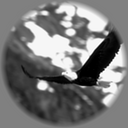
\includegraphics[scale = 0.26]{../../proposal/img3.png} & $\vec{x}_1 = $ 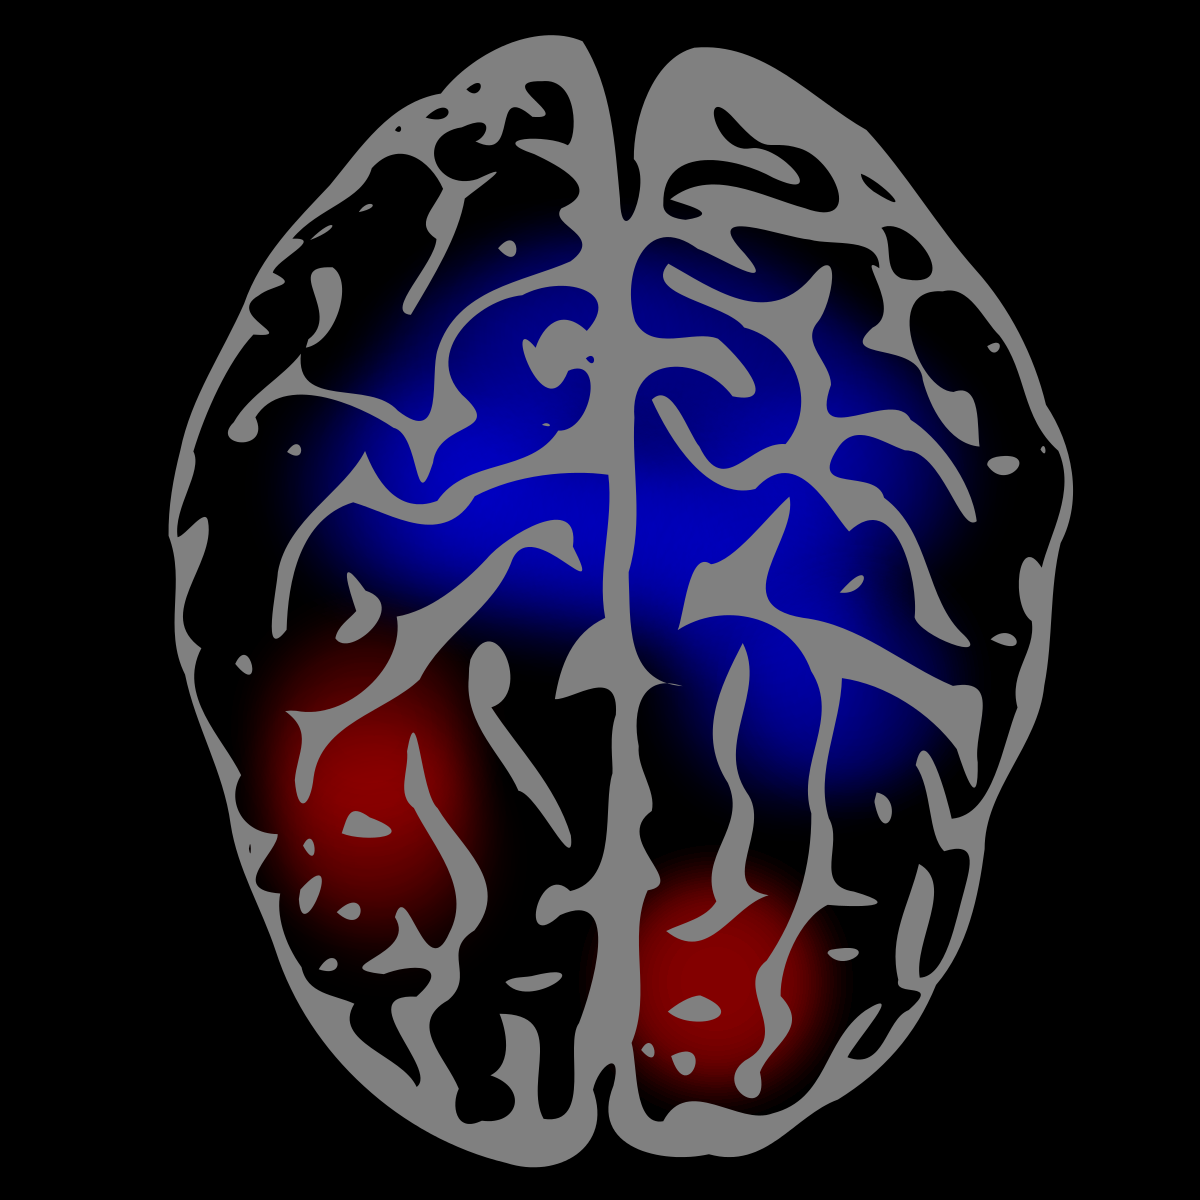
\includegraphics[scale = 0.035]{../../proposal/brain1.png} \\ \hline
2 & $y_2 = 2$ & 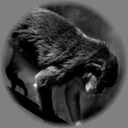
\includegraphics[scale = 0.26]{../../proposal/img4.png} & $\vec{x}_2 = $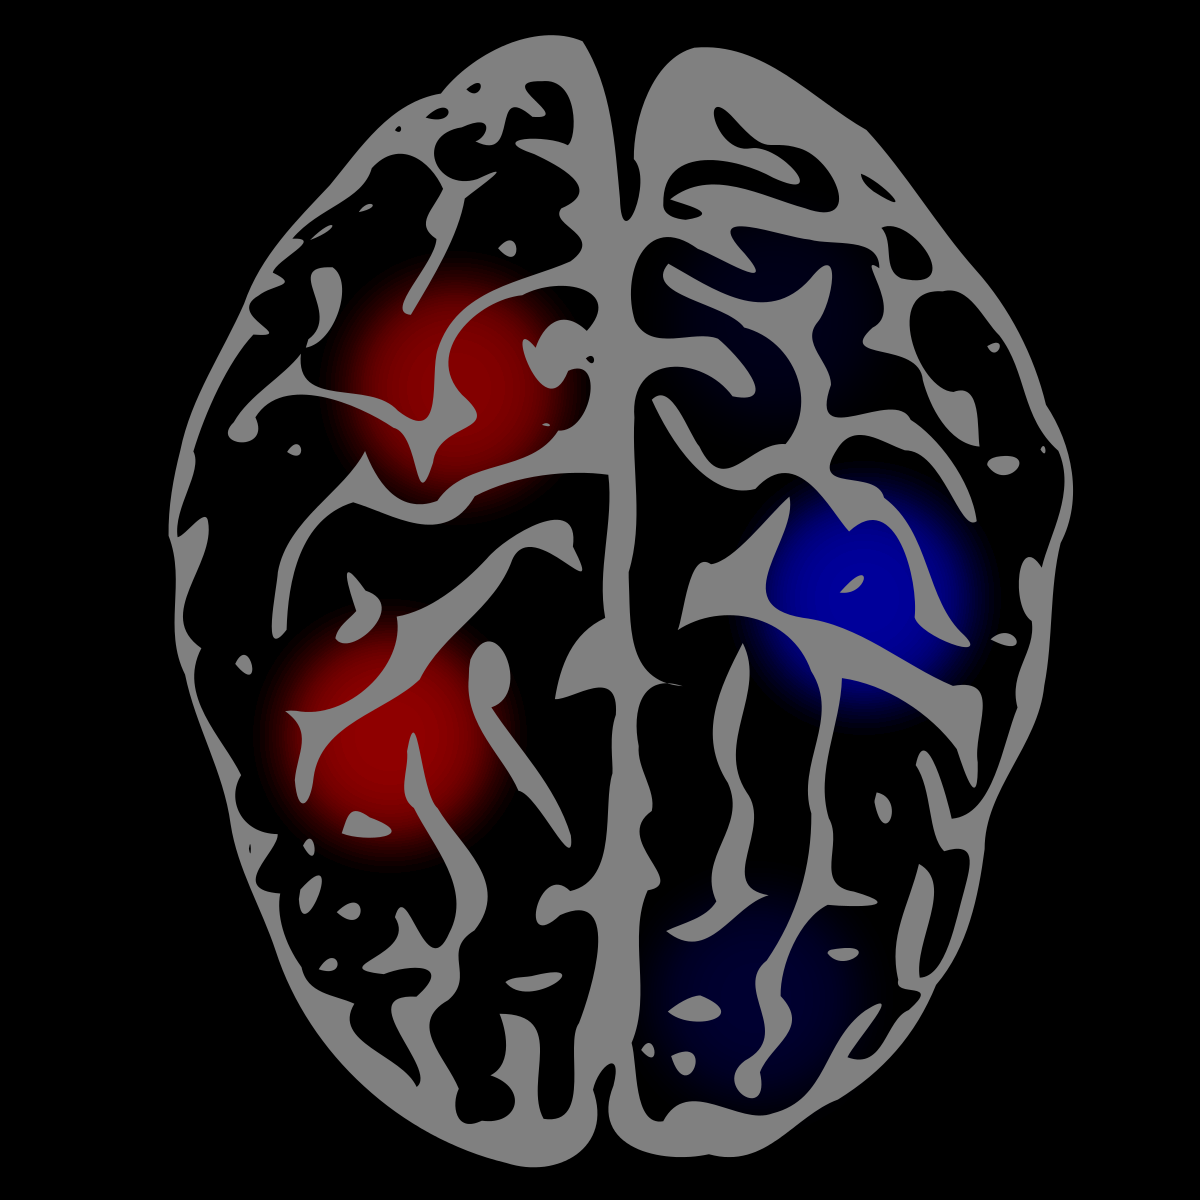
\includegraphics[scale = 0.035]{../../proposal/brain3.png} \\ \hline
3 & $y_3 = 1$ & 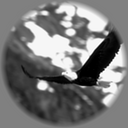
\includegraphics[scale = 0.26]{../../proposal/img3.png} & $\vec{x}_3 = $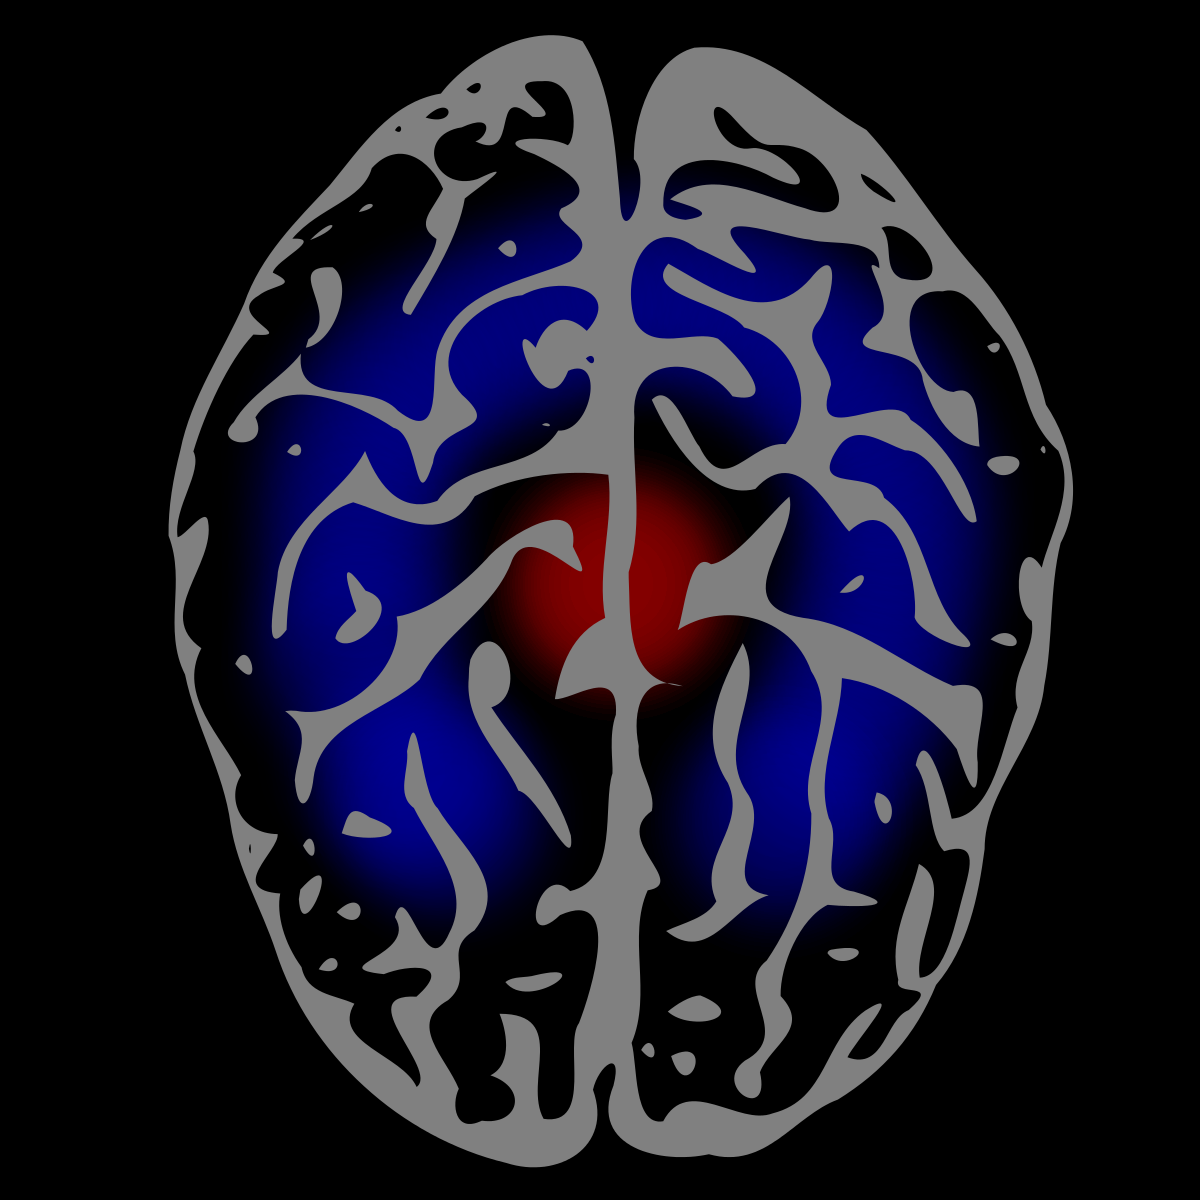
\includegraphics[scale = 0.035]{../../proposal/brain4.png} \\ \hline
4 & $y_4 = 2$ & 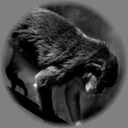
\includegraphics[scale = 0.26]{../../proposal/img4.png} & $\vec{x}_4 = $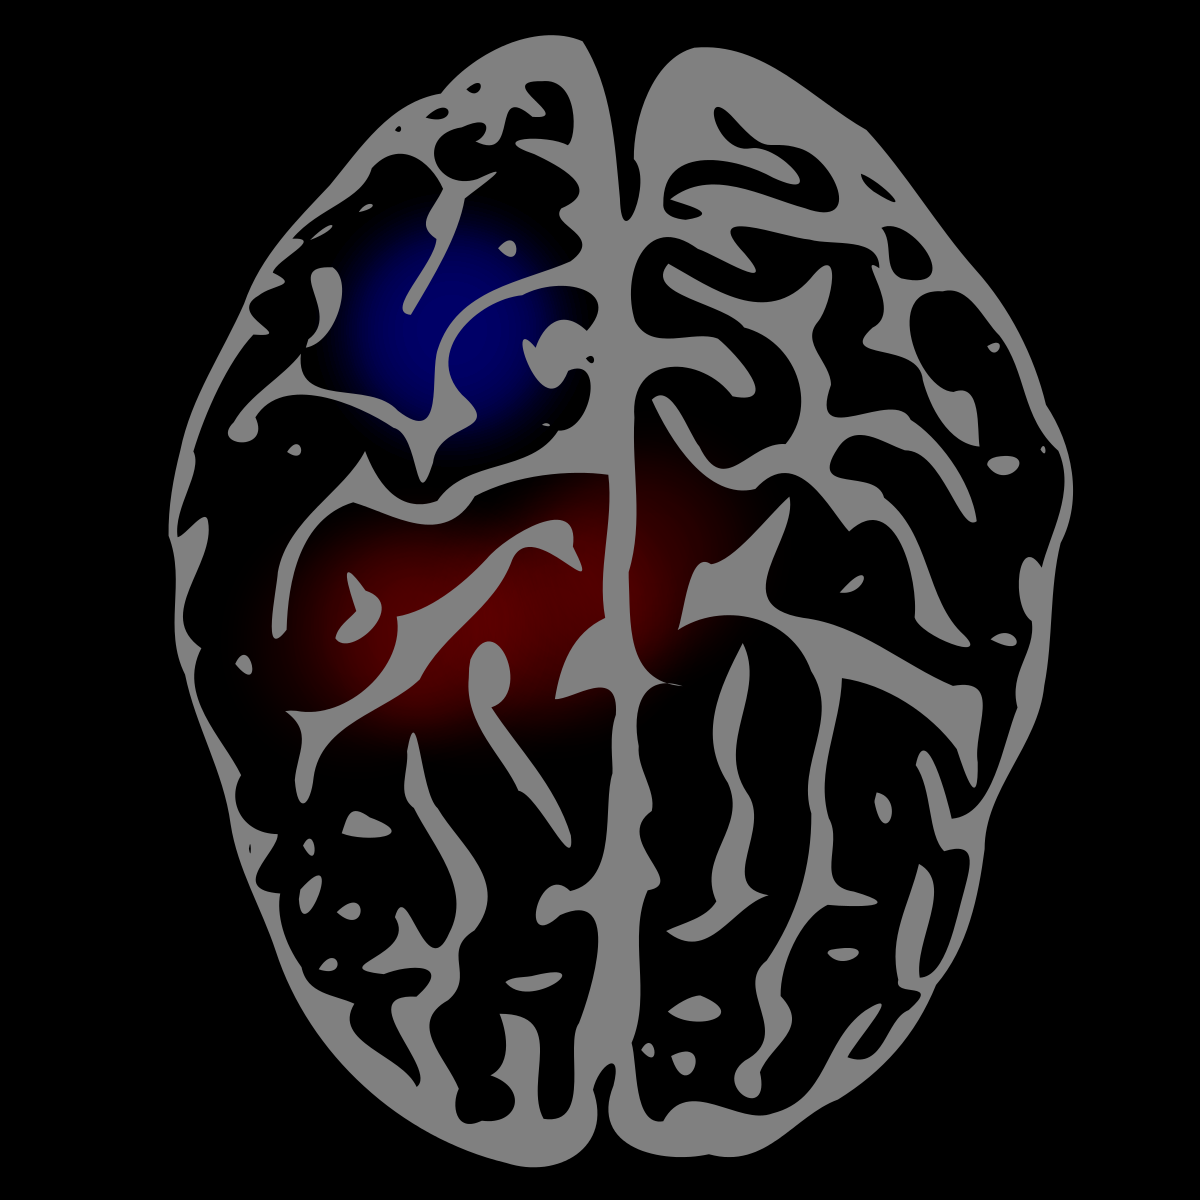
\includegraphics[scale = 0.035]{../../proposal/brain8.png} \\ \hline
\end{tabular}
\caption{Data output of a typical analysis of a task fMRI experiment.
  The raw data is processed to obtain a parametric map of inferred
  activation levels to each stimulus.  These activation levels are
  further utilized in downstream analyses. }
\label{fig:task_fmri}
\end{figure}

A number of statistical analyses can be performed on the
task-activation pairs $(y_i, \vec{x}_i)$.  The most common type of
analysis tests for significant \emph{peaks} of task-correlated
activity.  These analyses involve \emph{global} tests of the null
hypothesis of no correlation between task and activity.  However, MVPA
analyses tend to begin with local tests of independence between a
given region-of-interest (a cluster of neighboring voxels) and the
task.

\subsubsection{Classification-based test of independence}

A region of interest (ROI) is a collection of neighboring voxels,
chosen based on anatomical or geometric considerations.  To give a
concrete example, one can choose an arbitrary voxel in the brain, and
define an ROI as the set of all voxels within a given radius (say, $5
\text{mm}$) of the chosen voxel.  Recalling that $\vec{x}_i$ denotes
the activity level of the entire brain, let us write $\vec{x}_i^{ROI}$
for the subset of voxels in the brain map belonging to the ROI.

We would like to test the hypothesis of independence between the task
$Y$ and the joint activity level of the voxels belonging to the ROI,
considered as a random vector, $\vec{X}^{ROI}$.  While there are
numerous methods in the statistical literature for testing for
independence between a categorical random variable $Y$ and a random
vector $\vec{X}$, the approach taken in MVPA is typically to use
classification accuracies as the test statistic.

Recall that a classification rule is any (possibly stochastic) mapping
$f: \mathcal{X} \to \{1,\hdots, k\}$, where $k$ is the number of
levels of $Y$.  Let us assume that the $k$ different levels of $Y$
have the same number of repeats within the data.  The
\emph{generalization accuracy} of the classification rule is
\[
\text{GA}(f) = \frac{1}{k} \sum_{i=1}^k\Pr[f(\vec{X}^{ROI}) = i | Y = i].
\]
A trivial classification rule which outputs the result of a $k$-sided
die roll for all inputs $y$ would achieve a generalization accuracy of
$\text{GA} = \frac{1}{k}$.

Recall that the generalization accuracy of a data-dependent
classification rule $f$ can be obtained by using
\emph{data-splitting}, provided that the rule $f$ is constructed using
only the \emph{training data}.  Supposing that the original data
consists of pairs $(y_i,\vec{x}_i^{ROI})$ for $i = 1,\hdots, n$, let
$j_1,\hdots, j_{n_1}$ denote the $n_1$ randomly drawn training
indices, and $\ell_1,\hdots, \ell_{n_2}$ denote the $n_2$ randomly
drawn test indices.  The training data $(y_{j_i},
\vec{x}_{j_i}^{ROI})_{i=1}^{n_1}$ is used to construct a classification rule
$f$, while the test data is used to obtain a test accuracy $T$:
\[
T= \frac{1}{n_2} \sum_{i=1}^{n_2} I(f(\vec{x}_{\ell_i}^{ROI}) = y_{\ell_i}).
\]
%% also give the formula for stratifying by class

Under the null hypothesis $H_0: Y \perp \vec{X}^{ROI}$, the
generalization accuracy of any classification rule $f$ is equal to
$1/k$.  Therefore, we can write the null hypothesis as
\[
H_0: \text{GA}(f) = \frac{1}{k}
\]
and the alternative hypothesis as
\[
H_1: \text{GA}(f) > \frac{1}{k}.
\]

We will describe two different methods for testing $H_0$ versus $H_1$.
The first approach is to use the fact that the distribution of $T$ is
known under the null hypothesis.  The second approach is a permutation
test\footnote{Permutation tests are
widely used in statistical applications: for a good introduction to
the subject, the reader is invited to consult
\cite{efron1994introduction}.}.  The permutation test is more computationally expensive, but has
important advantages in terms of family-wise error control, as we will
describe in the sequel. %% describe in the next subsubsection

\emph{First approach.} Under the null hypothesis, using the fact that
the test observations $(y_{\ell_i}, \vec{x}_{\ell_i})$ are identical
and independently distributed from the population distribution of
stimulus-activity pairs, we have
\[
n_2 T \sim_{H_0} \text{Bernoulli}(n_2, \frac{1}{k})
\]
Therefore, let $c_\alpha$ be the $(1-\alpha)$ quantile of a
$\text{Bernoulli}(n_2, \frac{1}{k})$ distribution.  To perform a
hypothesis test at level $\alpha$, reject the null $H_0$ if $n_2 T >
c_\alpha$ and accept otherwise.  Equivalently, define the $p$-value as
the area under the tail of the $\text{Bernoulli}(n_2,
\frac{1}{k})$ distribution to the right of $T$,
\[
p = \Pr[X > n_2 T| X \sim \text{Bernoulli}(n_2, \frac{1}{k})],
\]
and reject if and only if $p < \alpha$.

\emph{Second approach (permutation test)}.  Under the null hypothesis of
independence between $Y$ and $\vec{X}^{ROI}$, the test statistic $T$
(the test accuracy on $n_2$ test observations) has a distribution that
is invariant under permutation of the labels $Y_1,\hdots, Y_n$.
Therefore, obtain $B$ samples of permutation test statistics
$T^{(1)},\hdots, T^{(B)}$ by the following procedure:
\begin{itemize}
\item[1.] For $j = 1,\hdots, B$, draw a random permutation $\sigma: n \to n$.
\item[2.] Use the pairs
  $(y_{\sigma_i},\vec{x}^{ROI}_{\sigma_i})_{i=1}^{n_1}$ to construct
  classification rule $f^{(j)}$ (using the same classifier as the one
  used to construct $f$).
\item[3.] Evaluate the test accuracy of $f^{(j)}$,
\[
T^{(j)}= \frac{1}{n_2} \sum_{i=1}^{n_2} I(f^{(j)}(\vec{x}_{\sigma_i}^{ROI}) = y_{\sigma_i}).
\]
\end{itemize}
The permutation $p$-value is calculated based on the rank of $T$ within the sample of permuation test statistics:
\[
p = \frac{\sum_{j=1}^B I(T^{(j)} < T) + 1}{B + 1},
\]
and reject the null hypothesis if and only if $p < \alpha$.

\subsubsection{Searchlight analysis}

Classifier-based tests of independence are commonly combined with the
\emph{multivariate searchlight} procedure
(\cite{kriegeskorte2006information}, \cite{kriegeskorte2007analyzing})
in order the scan the entire brain for informative clusters of voxels.
The procedure produces a 3D map of $p$-values in the brain, with
significant $p$-values indicative of regions in the brain associated
with the task.  Figure \ref{fig:searchlight_example} displays one
example of a $p$-value map obtained from an object perception task (\cite{chen2011cortical}).

\begin{figure}
\centering
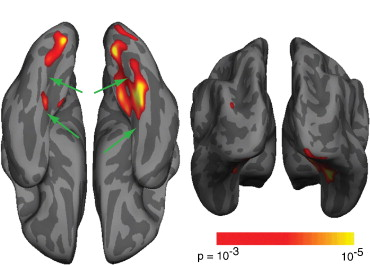
\includegraphics[scale = 0.5]{Figures/chen2010_cropped.png}
\caption{$p$-value map obtained from linear SVM-based searchlight
  applied to object perception data, using spherical neighborhoods
  with 9mm radius (\cite{chen2011cortical}).}
\label{fig:searchlight_example}
\end{figure}

A \emph{searchlight} refers to a local region-of-interest centered
around a particular \emph{central voxel}.  A variety of methods can be
used to define the neighborhood.  The most straightforward is the
\emph{spherical searchlight}, which fixes a radius $r$, and to include
all voxels within a distance $r$ of the central voxel.  However, more
sophisticated approaches may account for the geometry of the brain
surface (\cite{chen2011cortical}.)

Having chosen a method for obtaining searchlights, one generates a
searchlight centered around each voxel in the fMRI image, $\vec{x}$.
Let $\{ROI_1,\hdots, ROI_v\}$ denote the collection of such
searchlights, with $\vec{X}^{ROI_i}$ consisting of the voxels centered
around the $i$th voxel.

For each $ROI_i$, one conducts a hypothesis test for independence
between $Y$ and $\vec{X}^{ROI_i}$ using the local test of independence
described earlier.  % in the previous subsection This produces a map
of $p$-values, $p_1,\hdots, p_v$, for each voxel in the fMRI image.
Clusters of small $p$-values can be informally interpreted as
indicative of brain regions associated with the task.  Alternatively,
to test the global null hypothesis that all ROIs are independent of
the task, one can apply the permutation testing approach
simultaneously to all voxels in the brain.  The global permuation
approach is carried out as follows:
\begin{itemize}
\item[0.] (Non-permuted data): Draw a random permutation $\sigma: n \to n$. For $i = 1,\hdots, v$, use the pairs
  $(y_{\sigma_\ell},\vec{x}^{ROI_i}_{\sigma_\ell})_{\ell=1}^{n_1}$ to construct
  classification rule $f^{(0, i)}$
\item[1.] For $j = 1,\hdots, B$, draw a random permutation $\sigma: n \to n$.
\item[2.] For $i = 1,\hdots, v$, use the pairs
  $(y_{\sigma_\ell},\vec{x}^{ROI_i}_{\sigma_k})_{\ell=1}^{n_1}$ to construct
  classification rule $f^{(j, i)}$ (using the same classifier as the one
  used to construct $f$).
\item[3.] Evaluate the test accuracy $T^{(j,i)}$ of $f^{(j, i)}$.
\item[4.] Find the maximum accuracy $T^{(j)} = \max_{i=1}^v T^{(j,i)}$.
\item[5.] Define the $p$-value for each ROI by
\[
p_i =  \frac{\sum_{j=1}^B I(T^{(j)} < T^{(0, i)}) + 1}{B + 1},
\]
\end{itemize}
Since the permutations are shared across the ROIs, familywise control
is attained, in the sense that $p^* = \min_i p_i$ is a valid
$p$-value.

\subsection{Other applications}

Experimentally, mutual information has been used to detect strong
dependencies between stimulus features and features derived from
neural recordings, which can be used to draw conclusions about the
kinds of stimuli that a neural subsystem is designed to detect, or to
distinguish between signal and noise in the neural output.
Theoretically, the assumption that neural systems maximize mutual
information between salient features of the stimulus and neural output
has allowed scientists to predict neural codes from signal processing
models: for instance, the center-surround structure of human retinal
neurons matches theoretical constructions for the optimal filter based
on correlations found in natural images [cite].

\subsection{Can classification accuracy quantify information?}

Due to the analogy between the nervous system and a communications
network, it was a natural choice for early neuroscientists to adopt
Shannon's \emph{mutual information} as a quantitative measure of
dependence, as we saw in the application of mutual information to
decoding models (Section \ref{sec:model_selection}).  But as new
technologies enabled the recording of neural data at larger scales and
resolution, the traditional reductionist goals of neuroscience were
supplemented by increasingly ambitious attempts within neuroscience to
understand the dynamics of neural ensembles, and by efforts
originating within psychology and medicine to link the structure and
function of the entire human brain to behavior or disease.  The scale
of the data, and the complexity of the models studied posed an
obstacle to traditional information-theoretic approaches.  Therefore,
it was of considerable interest when Haxby (2001) introduced the usage
of \emph{supervised learning} (classification tasks) for the purpose
of quantifying stimulus information in task fMRI scans, as we
discussed in section \ref{sec:searchlight}.

Judging from the language used by the practioners themselves, it is
intuitively clear to them how classification accuracies can be used to
quantify information in brain scans.  We agree with the intuition
behind this practice, and go further to say that the use of
classification accuracies as a measure of information can be formally
justified.  However, having said this, it is important to remark that
Shannon's \emph{mutual information} need not be taken as the canonical
quantification of ``information'' as a measure of multivariate
dependence.  Instead, we take a step back and attempt to dissect the
intuitive properties of ``information'' and why the concept is useful
in science.  We will argue that given these intuitions, both mutual
information and classification accuracy can be seen as useful measures
of information.

\begin{itemize}
\item \emph{
Intuition 1: Information is a measure of dependence.}   If $\bX$ and $\bY$ are statistically independent, then
$\bX$ gives no information about $\bY$, and vice-versa.
\end{itemize}
This intuition is employed when researchers test the null hypothesis
of chance accuracy for classification.  If the null is accepted, the
researcher concludes that there is no information in the predictors
about the response.

\begin{itemize}
\item \emph{
Intuition 2a: Monotonicity with respect to inclusion of outputs.} If $\bX_1$ and $\bX_2$ are ensembles of neurons (or
individual neurons), then the combined ensemble $(\bX_1, \bX_2)$ has equal or
more information about $\bY$ than either component by itself.
\end{itemize}

\begin{itemize}
\item \emph{
Intuition 2b: Noise adds no information.} If, in the previous example, $\bX_2$ is independent of
$\bY$, then $\bX_2$ adds no information to the ensemble.
\end{itemize}
The non-informativity of noise is vital for the purpose of
\emph{localizing} information within fMRI voxels (as is done in
searchlight analysis.)  Since noise voxels fail to improve
classification performance (and indeed, sometimes harm empirical
performance,) the optimal searchlight radius will concentrate on
clusters of signal voxels, and minimize the inclusion of noise voxels.

\begin{itemize}
\item \emph{Intuition 3:}
Information can be used as a basis of model selection.  Among multiple
encoding/decoding models, a more accurate model should tend to have
greater information relative to less accurate models.  
\end{itemize}
Compared to the first two, this third intuition is somewhat less
obvious, but nevertheless appears as an important use-case for mutual
information, as seen in the application of mutual information to
choose encoding models.

%Arguably, both the application of mutual information described in
%\ref{sec:model_selection} and the use of classification accuracies in
%\ref{sec:searchlight} are justified by this common set of three
%intuitions.

It is well-known that the mutual information $I(\bX; \bY)$ satisfies
these three intuitions.  However, the \emph{Bayes classification
  accuracy}--the accuracy of the \emph{optimal} classifier, also
satifies these three intuitions.  
\begin{enumerate}
\item When $\bX$ and $\bY$ are
independent, then the Bayes accuracy falls to chance, $1/k$,
indicating `no information.'  
\item As additional predictors are made available, the Bayes accuracy
  can only improve.  As noise predictors are addded, the Bayes
  accuracy remains unchanged.
\item Supposing that there exists a `true encoding' with $\bY$ only
  depending on some function basis $\vec{b}(\bX)$, then the Bayes
  accuracy for predicting $\bY$ from the basis $\vec{g}(\bX)$ is
  maximized when $\vec{g} = \vec{b}$.
\end{enumerate}

However, an important caveat is that classification accuracies
attained in practice are at best an \emph{underestimate} of Bayes
accuracy, and therefore do not perfectly inherit all of the above
properties.  For instance, while the Bayes accuracy satisfies
Intuition 2b, classification accuracy generally does not: due to the
phenomenon of overfitting, the inclusion of noise predictors reduces
classification accuracy.

On the other hand, given sufficient training observations and
well-specification of models, classification accuracies begin to
approach Bayes accuracies, and therefore can be justifiable used as
measures of information which satisfy Intuitions 1-3.  This link
between empirical classification accuracies, Bayes accuracies, and
information forms the basis for much of the work in this thesis.

That said, a deeper understanding of the conditions which allow
attained classification accuracies to mimic the properties of Bayes
classification accuracy would be greatly useful for understanding the
practical limitations of some of the methods that will be proposed in
the later chapters.  However, we must leave this important work for
future research.



% Chapter 2

\chapter{Randomized classification} % Main chapter title

\label{Chapter2} % For referencing the chapter elsewhere, use \ref{Chapter1} 

As we foreshadowed in the introduction, randomized classification is
also one of the three methods we consider for evaluating
representations.  Yet, two other applications of randomized
classification are (i) for providing a formalism for evaluting
\emph{recognition systems}, and (ii) for studying generalizability of
certain classification-based experiments.  The application of
recognition systems provides the most intuitive way of understanding
the randomized classification task; therefore, in this chapter, we
begin with a discussion in section \ref{sec:recog_tasks} of
recognition tasks, and within this context, motivate the definition of
a randomized classification task in section \ref{sec:rc_motivation}.
We propose to use the randomized classification task to model the
problem of recognition, and to evalaute performance via the
\emph{average accuracy}.  Next, to put our ideas into practice, we
need ways to estimate the average accuracy from data, which we address
in \ref{sec:estimation_average_accuracy}.

Meanwhile, the problem of generalizing classification experiments
provides a natural motivation for studying the variance of
classification accuracy within a randomized classification task, which
we cover in section \ref{sec:average_bayes_accuracy}.  Meanwhile,
another one of the methods we consider--the identification task, is
closely connected with the randomized classification task.  We discuss
how our results in \ref{sec:average_bayes_accuracy} can also be
applied to the identification accuracy.

\section{Recognition tasks}\label{sec:recog_tasks}

Human brains have a remarkable ability to recognize objects, faces,
spoken syllables and words, and written symbols or words, and this
recognition ability is essential for everyday life.  While researchers
in artificial intelligence have attempted to meet human benchmarks for
these classical recognition tasks for the last few decades, only very
recent advances in machine learning, such as deep neural networks,
have allowed algorithmic recognition algorithms to approach or exceed
human performance (\cite{lecun2015deep}).

Within the statistics and machine learning literature, the usual
formalism for studying a recognition task is to pose it as a
\emph{multi-class classification} problem.  One delineates a finite
set of distinct entities which are to be recognized and distinguished,
which is the \emph{label set} $\mathcal{Y}$.  The input data is
assumed to take the form of a finite-dimensional real \emph{feature
  vector} $X \in \mathbb{R}^p$.  Each input instance is associated
with exactly one true label $Y \in \mathcal{Y}$.  The solution to the
classification problem takes the form of an algorithmically
implemented \emph{classification rule} $h$ that maps vectors $X$ to
predicted labels $\hat{Y} \in \mathcal{Y}$.  The classification rule
can be constructed in a data-dependent way: that is, one collects a
number of labelled \emph{training observations} $(X_1, Y_1)$ which is
used to inform the construction of the classification rule $h$.  The
quality of the classification rule $h$ is measured by \emph{generalization accuracy}
\[
\text{GA}(h) = \Pr[h(X) = Y],
\]
where the probability is defined with reference to the unknown
population joint distribution of $(X, Y)$.  

However, a limitation of the usual multi-class classification
framework for studying recognition problems is the assumption that the
label set $\mathcal{Y}$ is finite and known in advance.  When
considering human recognition capabilities, it is clear that this is
not the case.  Our ability to recognize faces is not limited to some
pre-defined, fixed set of faces; similarly with our ability to recognize
objects in the environment.  Humans learn to recognize novel faces and
objects on a daily basis.  And, if artificial intelligence is to fully
match the human capability for recognition, it must also possess the
ability to add new categories of entities to its label set over time;
however, at present, there currently exists a void in the machine
learning literature on the subject of the online learning of new
classes in the data.

The central theme of this thesis is the study of \emph{randomized
  classification}, which can be motivated as an extension of the
classical multi-class classification framework to accommodate the
possibility of growing or infinite label sets $\mathcal{Y}$. The basic
approach taken is to assume an infinite or even continuous label space
$\mathcal{Y}$, and then to study the problem of classification on
finite label sets $S$ which are randomly sampled from $\mathcal{Y}.$
This, therefore defines a \emph{randomized classification} problem
where the label set is finite but may vary from instance to instance.
One can then proceed to answer questions about the variability of the
performance due to randomness in the labels, or how performance
changes depending on the size of the random label set.

\section{Randomized classification}\label{sec:rc_motivation}

\subsection{Motivation}
The formalism of classification is inadequate for studying many
practical questions related to the generalizability of the facial
recognition system.  Using test data, we estimate the generalization
accuracy of a recognition system.  However, these estimated accuracies
apply only to the particular collection of individuals
$\{y^{(1)},\hdots, y^{(k)}\}$.  If we were to add a new individual
$y^{(k+1)}$ to the dataset, for instance, when photographs are
uploaded on Facebook containing a new user, this defines a totally new
classification problem because the expanded set of labels
$\{y^{(1)},\hdots, y^{(k+1)}\}$ defines a different response space
than the old set of labels $\{y^{(1)},\hdots, y^{(k)}\}$.  Yet, these
two classification problems are clearly linked.  To take another
example, a client might want to run a facial recognition system
developed by lab A on their own database of individuals.  In this
case, there might be no overlap between the people in lab A's database
and the people in the client's database.  And yet, the client might
still expect the performance figures reported by lab A to be
informative of how well the recognition system will do on their own
database!

The question of how to link performance between two different but
related classification tasks is an active area of research, known as
\emph{transfer learning}.  But while the two examples we just listed
might be considered as examples of transfer learning problems, the
current literature on transfer learning, as far as we know, does not
study the problem of \emph{mutating label sets}.  Therefore, to
address this new class of questions about the generalizability of the
recognition system, we need to formalize our notions of (a) what
constitutes a `recognition system' which can be applied to different
classification problems, and (b) what assumptions about the problem,
and what assumptions about the classifiers used, allow one to infer
performance in one classification problem based on performance in
another classification problem.

\subsection{Setup}
By `recognition system,' we really mean a \emph{learning algorithm}
$\Lambda$ which can take training data as input, and produce a
classification rule for recognizing faces.  While a classification
rule is bound to a specific label set, a learning algorithm can be
applied to datasets with arbitrary label sets, and be continually
updated as new labels are added to the label set.  To `update' a
facial recognition system with new data means to apply the learning
algorithm to the updated database.

Now we can formalize what it means to generalize performance from one
problem to another.  A \emph{classification problem} $P$ is specified
by a label set $\mathcal{Y}$, a predictor space $\mathcal{X}$, a joint
distribution $G$ on $\mathcal{X} \times \mathcal{Y}$, and a
\emph{sampling scheme} $S$ for obtaining training data (for example,
to obtain $n$ observations from $G$ i.i.d.).  The sampling scheme is
needed because we cannot say much about how the learning algorithm
will perform unless we know how much training data it is going to
have.  The generalization accuracy (GA) of the algorithm $\Lambda$ on the
classification problem $P = (\mathcal{Y}, \mathcal{X}, G, S)$ is
defined as the expected risk of the resulting classification rule $h$,
\[
\text{GA}_P(\Lambda) = \E[\text{GA}(h)]
\]
where $h$ is produced by applying $\Lambda$ to the training data,
sampled by $S$.  The expectation is taken over the randomness in the
generation of the training data.

At this point we have defined a general transfer learning
problem: given two different classification problems $P_1 =
(\mathcal{Y}_1, \mathcal{X}_1, G_1, S_1)$ and $P_2 = (\mathcal{Y}_2,
\mathcal{X}_2, G_2, S_2)$, what can we say about the relationship
between $\text{GA}_{P_1}(\Lambda)$ and $\text{GA}_{P_2}(\Lambda)$?
Not much, unless we make many more assumptions about how $P_1$ and
$P_2$ are linked.

The basic approach we will take is to assume that both $P_1$ and $P_2$
have been generated randomly via a common mechanism.  In the original
motivating context of facial recognition, this is to say that two
different label sets $\mathcal{Y}_1$ and $\mathcal{Y}_2$ are linked
because they both belong to a common population of labels
$\mathcal{Y}$, i.e., the population of all possible humans, and to
further assume that both have been \emph{sampled}, in the same manner,
from $\mathcal{Y}$.

The study of how to make inferences about the risk in $P_2$ given
information about the performance achieved in $P_1$, granted a set of
assumptions on how $P_1$ and $P_2$ have been randomly generated (and
are thereby linked through shared randomization mechanisms) forms the
basis of the subject of \emph{randomized classification}.

As we noted in the introduction, the problem of randomized
classification has a close ancestor in the study of \emph{random code
  models} in information theory.  There, the problem is to understand
the \emph{decoding performance} (the analogue to risk) of a
encoding/decoding system $P$ which has a randomized code space
$\mathcal{Y}$.  Where random code models have a random codebook which
is a sample over a distribution of all possible codes, randomized
classification problems have a random label set that is a sample of a
larger label space.  However, the results we obtain for randomized
classification are more general in nature than the existing results
availible for random code models, because work on random codes is
generally limited to asymptotic settings, whereas we obtain finite-$k$
results, and because random code models assume a specific
product-distribution structure on $(X, Y)$ which is not appropriate
for classification problems.

\subsection{Assumptions}

The randomized classification model we study has the following
features.  We assume that there exists an infinite (or even
continuous) label space $\mathcal{Y}$ and a response space
$\mathcal{X} \in \mathbb{R}^p$.  For each label $y \in \mathcal{Y}$,
there exists a distribution of features $F_y$.  That is to say, that
for a feature-label pair $(X, Y)$, that the conditional distribution
of $X$ given $Y = y$ is given by $F_y$.  Furthermore, we assume that
there exists a prior distribution $\pi$ on the label space $\mathcal{Y}$.

A random classification task $P$ can be generated as follows.  The
label set $\mathcal{S} = \{Y^{(1)},\hdots, Y^{(k)}\}$ is generated by
drawing labels $Y^{(1)},\hdots, Y^{(k)}$ i.i.d. from $\pi$.  The joint
distribution $G$ of pairs $(X, Y)$ is uniquely specified by the two
conditions that (i) the marginal distribution of $Y$ is uniform over
$\mathcal{S}$, and (ii) the conditional distribution of $X$ given
$Y=Y^{(i)}$ is $F_{Y^{(i)}}$.  We sample both a training set and a
test set.  The training set is obtained by sampling $r_1$ observations
$X_{j, train}^{(i)}$ i.i.d. from $F_{Y^{(i)}}$ for $j = 1,\hdots,
r_1$.  The test set is likewise obtained by sampling $r_2$
observations $X_j^{(i)}$ i.i.d. from $F_{Y^{(i)}}$ for $j = 1,\hdots,
r_2$.  For notational convenience, we represent the training set as
the set of empirical distributions $\{\hat{F}_{Y^{(i)}}\}_{i=1}^k$
where
\[
\hat{F}_{Y^{(i)}} = \frac{1}{r_1} \sum_{j=1}^{r_1} \delta_{X^{(i)}_{j, train}}.
\]
Figure \ref{fig:training_set} illustrates the sampling scheme for
generating the training set.

\begin{figure}[h]
\centering
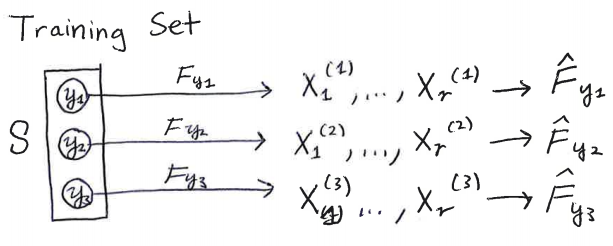
\includegraphics[scale = 0.4]{../extrapolation_figures/training_set.png}
\caption{Training set}\label{fig:training_set}
\end{figure}

Our analysis will also rely on a property of the classifier. We do not
want the classifier to rely too strongly on complicated interactions
between the labels in the set. We therefore propose the following
property of marginal separability for classification models:

\begin{definition}
\begin{enumerate}
\item The classification rule $h$ is called a \emph{marginal rule} if 
\[
h(x) = \text{argmax}_{y \in \mathcal{S}} m_y(x),
\]
where the function $m_y$ maps $\mathcal{X}$ to $\mathbb{R}$. 
\item Define a marginal model $\mathcal{M}$ as a mapping from empirical distributions
to margin functions,
\[
\mathcal{M}(\hat{F}_y) = m_y(x).
\]
\item A classifier that produces marginal classification rules
\[
h(x) = \text{argmax}_{y \in \mathcal{S}} m_y(x),
\]
by use of a marginal model, i.e. such that
$m_y=\mathcal{M}(\hat{F}_y)$ for some marginal model $\mathcal{M}$,
is called a \emph{marginal classifier}.
\end{enumerate}
\end{definition}
In words, a marginal classification rule produces a \emph{margin}, or
score, for each label, and chooses the label with the highest
margin. The marginal model converts empirical distributions
$\hat{F_y}$ over $\mathcal{X}$ into the margin function
$m_y$.  The \emph{marginal} property allows us to prove strong results
about the accuracy of the classifier under i.i.d. sampling assumptions.

\textbf{Comments:}
\begin{enumerate}
\item The marginal model includes several popular classifiers.
A primary example for a marginal model is the estimated Bayes
classifier. Let $\hat{f_y}$ be a density estimate obtained from the
empirical distribution $\hat{F_y}$. Then, we can use the estimated
densities of each class to produce the margin functions:
\[ m^{EB}_y(x) = \log(\hat{f_{y}}(x)).\]
The resulting empirical approximation for the Bayes classifier
(further assuming a uniform prior $\pi$) would be
\[ f^{EB}(x) = \text{argmax}_{y \in \mathcal{S}}(m^{EB}_y(x)).\]
\item Both the Quadratic Discriminant Analysis and the naive Bayes classifiers can be seen as specific instances of an estimated Bayes classifier
\footnote{QDA is the special case of the estimated Bayes classifier when $\hat{f_y}$ is obtained as
the multivariate Gaussian density with mean and covariance parameters estimated from the data.
Naive Bayes is the estimated Bayes classifier when $\hat{f_y}$ is obtained as the product of estimated componentwise marginal distributions
of $p(x_i|y)$}. 
For QDA, the margin function is
given by
\[
m_y^{QDA}(x) = -(x - \mu(\hat{F}_y))^T \Sigma(\hat{F}_y)^{-1} (x-\mu(\hat{F}_y)) - \log\det(\Sigma(\hat{F}_y)),
\]
where $\mu(F) = \int y dF(y)$ and $\Sigma(F) = \int (y-\mu(F))(y-\mu(F))^T dF(y)$.
In Naive Bayes, the margin function is
\[
m^{NB}_y(x) = \sum_{i=1}^n \log \hat{f}_{y, i}(x),
\]
where $\hat{f}_{y, i}$ is a density estimate for the $i$-th component of
$\hat{F}_y$.
\item There are also many classifiers which do not satisfy the marginal property, such as multinomial logistic regression,
multilayer neural networks, decision trees, and k-nearest neighbors.
\end{enumerate}

The operation of a marginal classifier is illustrated in figure
\ref{fig:classification_rule}.  Since a marginal classifier is
specified entirely by its marginal model $\mathcal{M}$, we will take
the notational convention of referring to a marginal classifier as
$\mathcal{M}$.

\begin{figure}[h]
\centering
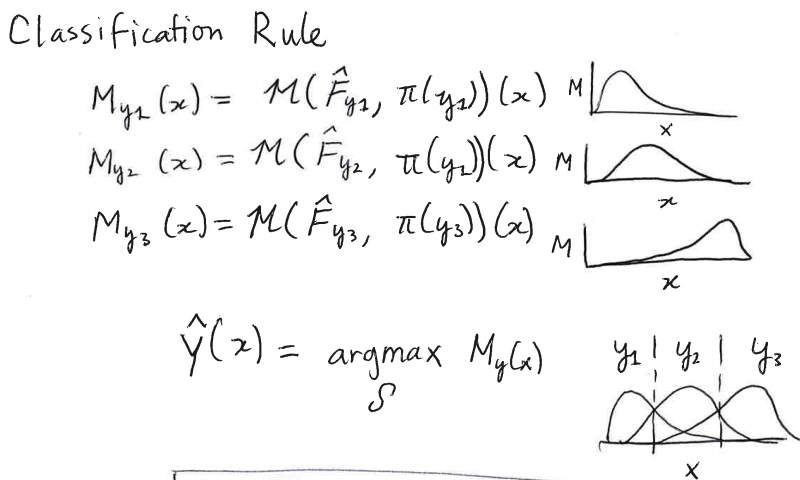
\includegraphics[scale = 0.4]{../extrapolation_figures/classification_rule.png}
\caption{Classification rule}\label{fig:classification_rule}
\end{figure}

We would like to identify the sources of randomness in evaluating a
classifier.  First, there is the specific choice of $k$ classes for
the label set.   Second, there is randomness in training the classifier
for these classes, which comes from the use of a finite training
set. Third, there is the randomness in the estimated risk when
testing the classifier on a test set.

If we \emph{fix} a particular realization of the random label set
$\mathcal{S} = \{y^{(1)}, \hdots, y^{(k)}\}$ as well as the training
set $\{\hat{F}_{y^{(i)}}\}_{i=1}^k$, then the classifier $h(x)$ is
fixed, and only the third source of randomness (in test risk) applies.
However, the true generalization accuracy of the classifier is deterministic:
\begin{align*}
\text{GA}(h) &= \Pr[Y = h(X)|Y \sim \text{Unif}(\mathcal{S}),
  \mathcal{S}, \{\hat{F}_{y^{(i)}}\}_{i=1}^k] 
\\&= \frac{1}{k}
\sum_{i=1}^k \Pr[m_{y^{(i)}}(x) = \max_j m_{y^{(j)}}(x)|X \sim
  F_{y^{(i)}}, \mathcal{S}, \{\hat{F}_{y^{(i)}}\}_{i=1}^k].  
\\&= \frac{1}{k}
\sum_{i=1}^k \int_{\mathcal{X}} I(m_{y^{(i)}}(x) = \max_j m_{y^{(j)}}(x)) dF_{y^{(i)}}(x),
\end{align*}
recalling that $m_{y^{(i)}}(x) \stackrel{def}{=}
\mathcal{M}(\hat{F}_{y^{(i)}})(x)$ is the margin function obtained
from the training data of the $i$th class.

If we \emph{fix} a particular realization of the random label set
$\mathcal{S} = \{y^{(1)}, \hdots, y^{(k)}\}$, then we can define the
(generalization) accuracy specific to that label set.  However, the
training data $\{\hat{F}_{y^{(i)}}\}_{i=1}^k$ will be random.  Let us
denote the \emph{distribution} of the empirical distribution
$\hat{F}_y$ constructed from sample size $r$ as $\Pi_{y, r}$.  The
accuracy of the classifier $\mathcal{M}$ on label set $\mathcal{S}$ is
given by
\begin{align*}
\text{GA}_{\mathcal{S}}(\mathcal{M}) &= \Pr[Y = h(X)|Y \sim
  \text{Unif}(\mathcal{S}), \hat{F}_{y^{(i)}} \sim \Pi_{y^{(i)}, r_1}] \\&= \frac{1}{k} \sum_{i=1}^k \int
I(\mathcal{M}(\hat{F}_{y^{(i)}})(x) = \max_j
\mathcal{M}(\hat{F}_{y^{(j)}})(x)) dF_{y^{(i)}}(x) \prod_{\ell=1}^k
d\Pi_{y^{(\ell)}, r_1}(\hat{F}_{y^{(\ell)}}).
\end{align*}
The calculation of the accuracy (for fixed label set $\mathcal{S}$) is
illustrated in figure \ref{fig:risk}.

\begin{figure}[h]
\centering
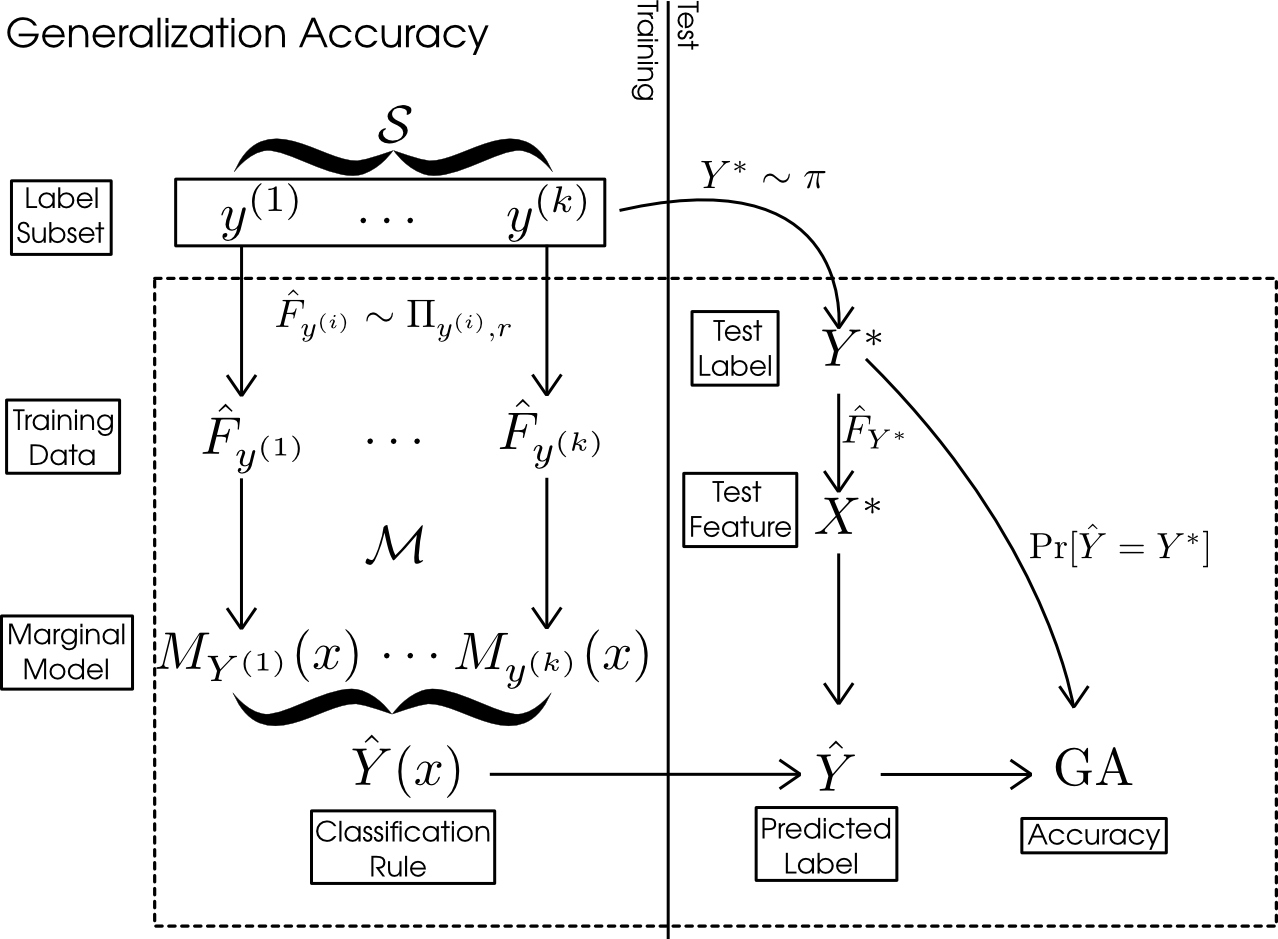
\includegraphics[scale = 0.3]{../extrapolation_simple/risk.png}
\caption{Generalization accuracy}\label{fig:risk}
\end{figure}

Finally, suppose we do not fix any of the random quantities in the
classification task $P$, and merely specify $k$, the number of
classes, and $r_1$, the number of repeats in the training set.  
Then the $k$-class, $r$-repeat \emph{average generalization accuracy} of
a marginal classifier $\mathcal{M}$ is defined as
\begin{align*}
\text{AGA}_{k,r_1}(\mathcal{M}) &= \E[\text{GA}_{\mathcal{S}}(\mathcal{M})|Y^{(1)}, \hdots, Y^{(k)} \sim \pi]
\\&= \frac{1}{k} \sum_{i=1}^k \int
I(\mathcal{M}(\hat{F}_{y^{(i)}})(x) = \max_j
\mathcal{M}(\hat{F}_{y^{(j)}})) dF_{y^{(i)}}(x) \prod_{\ell=1}^k
d\Pi_{y^{(\ell)}, r_1}(\hat{F}_{y^{(\ell)}}) d\pi(y^{(\ell)}).
\\&= \int
I(\mathcal{M}(\hat{F}_{y^{(1)}})(x) = \max_j
\mathcal{M}(\hat{F}_{y^{(j)}})) dF_{y^{(1)}}(x) \prod_{\ell=1}^k
d\Pi_{y^{(\ell)}, r_1}(\hat{F}_{y^{(\ell)}}) d\pi(y^{(\ell)}).
\end{align*}
where the last line follows from noting that all $k$ summands in the previous line are identical.
The definition of average generalization accuracy is illustrated in Figure \ref{fig:average_risk}.

\begin{figure}[h]
\centering
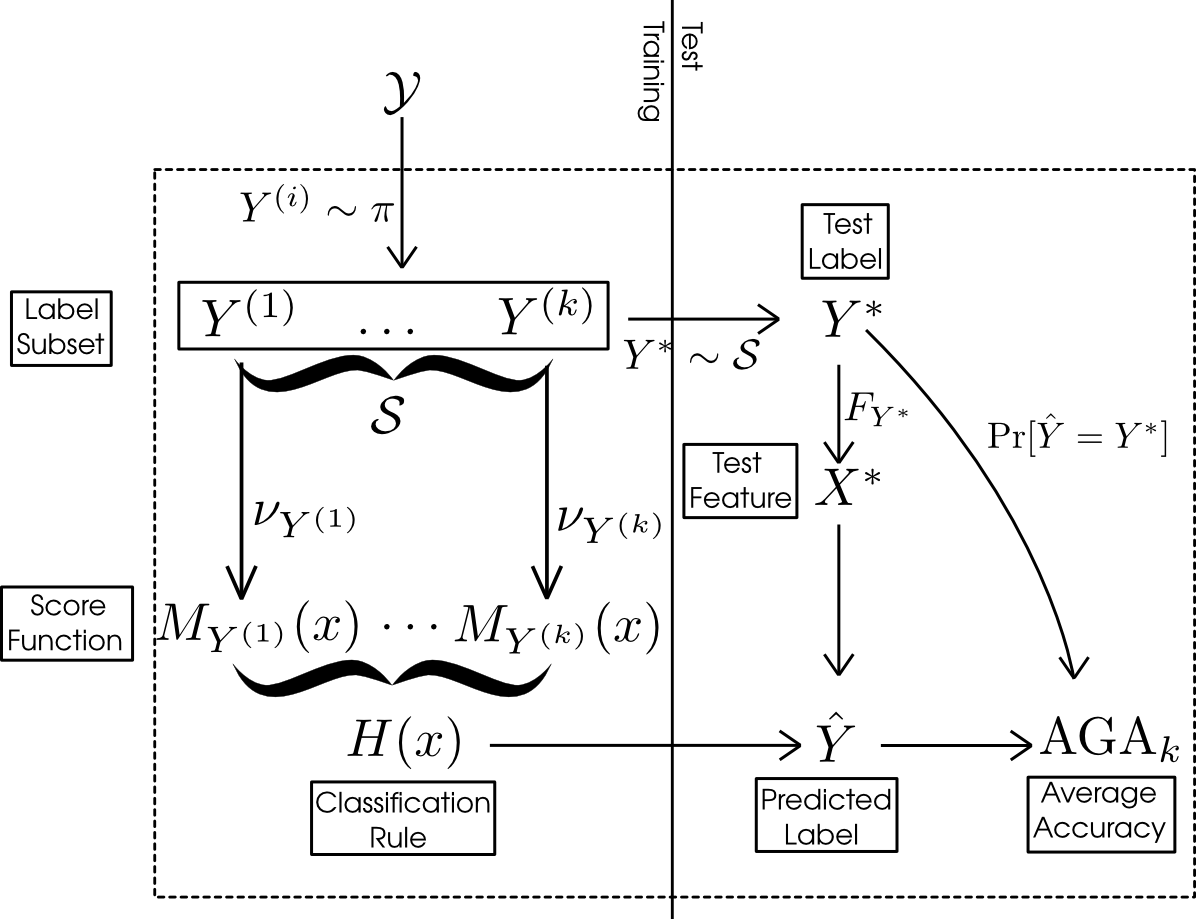
\includegraphics[scale = 0.3]{../extrapolation_simple/average_risk.png}
\caption{Average generalization accuracy}\label{fig:average_risk}
\end{figure}

Having defined the average (generalization) accuracy for the randomized classification
task, we begin to develop the theory of how to \emph{estimate} the
average accuracy in the next section.

\section{Estimation of average accuracy}\label{sec:estimation_average_accuracy}

Suppose we have training and test data for a classification task $P_1$
with $k_1$ classes, $r_1$-repeat training data and $r_2$-repeat test
data.  That is, we have label set $\mathcal{S}_1 =
\{y^{(i)}\}_{i=1}^{k_1}$, as well as training sample $\hat{F}_{y^{(i)}}$
and test sample $(x_1^{(i)},\hdots, x_{r_2}^{(i)})$ for $i =
1,\hdots, k_1$.  How can we estimate the $k, r$-average accuracy of a
marginal classifier $\mathcal{M}$ for arbitrary $k$ and $r$?

Let us start with the case $k = k_1$ and $r = r_1$.  Then the answer
is simple: construct the classification rule $h$ using marginal model
$\mathcal{M}$ from the training data.  Then the test accuracy of $h$ is an
unbiased estimator of $\text{AGA}_{k,r}$.

This follows from definition.  Observe that $\text{AGA}_{k_1,r_1}$ is
the expected prediction risk for the classification rule $h$ for a
randomized classification problem $P$ with $k_1$ classes and
$r_1$-repeat training data.  Of course, the classification task $P_1$
that we have been given is a random draw from the desired
distribution of random classification problems.  Therefore, the
prediction risk of $h$ constructed from $P_1$ is unbiased for
$\text{AGA}_{k_1, r_1}$, and since test accuracy is unbiased for
generalization accuracy, it follows that the test accuracy of $h$ is
an unbiased estimator of $\text{AGA}_{k,r}$, as we claimed.

In following sections, we consider more complicated cases where $k_1
\neq k$.  However, before proceeding, let us first review the
procedure for computing the test accuracy.

For any given test observation $x_j^{(i)}$, we obtain the predicted
label $\hat{y}_j^{(i)}$ by computing the margin for each class,
\[
M_{i,j,\ell} = \mathcal{M}(\hat{F}_{y^{(\ell)}})(x_j^{(i)}) =  m_{y^{(\ell)}}(x_i^{(j)}),
\]
for $\ell = 1,\hdots, k_1$,
and by finding the class with the highest margin $M_{i, j, \ell}$,
\[
\hat{y}_j^{(i)} = y^{(\argmax_\ell M_{i, j, \ell})}.
\]
The test accuracy is the fraction of correct classification over test observations,
\begin{equation}
\text{TA} = \frac{1}{r_2k_1} \sum_{i=1}^{k_1} \sum_{j=1}^{r_2} I(\hat{y}_j^{(i)} = y^{(i)}).
\end{equation}
For each test observation, define the ranks of the margins by
\[
R_{i,j,\ell} = \sum_{m \neq \ell} I\{M_{i,j,\ell} \geq M_{i, j, m}\}.
\]
Therefore, $\hat{y}_j^{(i)}$ is equal to $y^{(i)}$ if and only if $R_{i,j,i} = k_1$.
Thus, an equivalent expression for test accuracy is
\begin{equation}\label{eq:test_risk}
\text{TA} = \frac{1}{r_2 k_1} \sum_{i=1}^{k_1} \sum_{j=1}^{r_2} I\{R_{iji} = k_1\}.
\end{equation}

\subsection{Subsampling method}

Next, let us consider the case where $k < k_1$ and $r=r_1$.  Define a
classification problem $P_2$ with label set $\mathcal{S}_2$ obtained
by sampling $k$ labels uniformly without replacement from
$\mathcal{S}_1$.  Let the training and test data for $P_2$ be obtained
by taking the training data and test data from $P_1$ belonging to
labels in $\mathcal{S}_1$.  It follows that $P_2$ is a randomized
classification task with $k$ labels, $r_1$-repeat training data and
$r_2$-repeat test data.  Therefore, by the previous argument, the test
accuracy for a classification rule $h$ constructed using the training data
in $P_2$ provides an unbiased estimate of $\text{AGA}_{k, r_1}$.

However, we can get a much better unbiased estimate of
$\text{AGA}_{k, r_1}$ by averaging over the randomization of
$\mathcal{S}_2$.  Na\"{i}vely, this requires us to train and evaluate
${k_1}\choose{k}$ classification rules.  However, due to the special
structure of marginal classifiers, we do the computation in the same
order of computation as evaluating a single classification rule
(assuming that the computational bottleneck is in training the
classifier.)

This is because the rank $R_{iji}$ of the correct label, $i$, for the
$x_j^{(i)}$ allows us to determine how many subsets $\mathcal{S}_2$
will result in a correct classification.  For example $x_j^{(i)}$,
there are $R_{iji} - 1$ labels with a lower margin than the correct
label $i$.  Therefore, as long as one of the classes in
$\mathcal{S}_2$ is $i$, and the other $k-1$ labels are from the set of
$R_{iji}-1$ labels with lower margin than $i$, the classification of
$x_j^{(i)}$ will be correct.  This implies that there are
${R_{iji}-1}\choose{k-1}$ such subsets $\mathcal{S}_2$ where
$x_j^{(i)}$ is classified correctly, and therefore

\begin{equation}\label{eq:avtestrisk}
\text{AverageTA}_{k, r_1} = \frac{1}{{{k_1}\choose{k}}}\frac{1}{r_2 k} \sum_{i=1}^{k_1} \sum_{j=1}^{r_2} {{R_{iji}-1}\choose{k-1}}.
\end{equation}

\subsection{Extrapolation}

A much more challenging case is when $k_2 > k_1$: that is, we want to
predict the performance of the classification model in a setting with
more labels than we currently see in the training set.  This is the
subject of Chapter 3.

\subsection{Variance bounds}

By now we have developed unbiased estimators for average generalization accuracy in the
special case $k \leq k_1$, and the following chapter will present
methods for the more difficult case $k > k_1$.  However, to get useful
inference statements, we also have to understand the variance of these
estimators.  For the large part, this is still work-in-progress.
However, some first steps towards addressing this problem are
described in the next section.

\section{Reproducibility and Average Bayes accuracy}\label{sec:average_bayes_accuracy}

\subsection{Motivation}

In task fMRI experiments, one typically obtains data of the form
$(\vec{x}_i, y_i)$, where $\vec{x}_i$ are activity patterns obtained
from the fMRI scan for a region of interest, and $y_i$ are categories
for tasks.  The labels $y_i$ are limited to a discrete label set
$\mathcal{S} = \{y^{(1)},\hdots, y^{(k)}\}$.  Data-splitting is used
to obtain a test accuracy $\text{TA}$ for predicting $y$ from
$\vec{x}$.  The test accuracy is then interpreted as evidence for the
specialization of that region of interest for the task at hand: a high
accuracy suggests that the region is specialized for the task, while a
low accuracy suggests that the region is not specialized for the task.

However, a limitation of this approach is the poor reproducibility of
the test accuracy $\text{TA}$.  Besides the dependence of $\text{TA}$
on the particular subject participating in the experiment, the
randomness in sampling training and test data, and the classifier
used, there is an even more fundamental issue in that the
classification task is often inconsistent from lab to lab.  That is
because the task exemplars--that is, the set of labels
$\{y^{(i)}\}_{i=1}^k$, may be arbitrarily specified, and therefore
even ignoring the effect of subject, sampling of the data, and
classifier, the generalization accuracy depends on an arbitrary choice
of exemplars.

On the other hand, fixing in advance the set of exemplars
$\{y^{(i)}\}_{i=1}^k$ is also not a satisfactory solution, since the
objective of the experiment is to understand the general relation
between the task and the region of interest, and not the relationship
between a particular set of task exemplars $\{y^{(i)}\}_{i=1}^k$ and
the region of interest.

Randomized classification provides a solution for addressing both the
variability in estimation target and generalization to the population,
as long as one can justify the assumption that the labels
$\{y^{(i)}\}_{i=1}^k$ are a random sample from some population of task
exemplars $\pi$.  While the generalization accuracy $\text{GA}$ for
any particular, fixed set of exemplars is \emph{not} a population
parameter, the average generalization accuracy $\text{AGA}$ \emph{is}
defined with reference to a population, albeit also dependent on a
specific classifier and sampling scheme.  Meanwhile, the limitations
on reproducibility due to differing choices of labels sets can be
understood based on the variability properties of $\text{GA}$.

However, one can argue that randomized classification does not go far
enough to ensure generalizability of results, because $\text{AGA}$
still depends on the sampling scheme (the amount of training data) and
the choice of classifier, which are both arbitrary experimental
choices.  Therefore, our proposal is to treat the average \emph{Bayes}
accuracy as the estimation target of interest.  The average Bayes
accuracy is defined independently of the classifier and sampling
scheme, and we will develop tools for inferring probabilistic lower
bounds (lower confidence bounds) of the average Bayes accuracy in this
section.

\subsection{Setup}

%% todo: switch notations in this section

Define the generalization accuracy of a classification rule $f$ as the complement
of its risk (under zero-one loss),
\[
\text{GA}(f) = \Pr[Y = f(X)].
\]

The generalization accuracy of any classification rule is
upper-bounded by the accuracy of the optimal classification rule, or
\emph{Bayes rule.}  That is, one can define the \emph{Bayes accuracy}
as
\[
\text{BA} = \sup_f \text{GA}(f).
\]
And due to Bayes' theorem, the optimal classification rule $f^*$ which
achieves the Bayes accuracy can be given explicitly: it is the maximum a
posteriori (MAP) rule
\[
f^*(x) = \argmax_{i=1}^k\ p(x|y^{(i)}).
\]
Of course, it is not possible to construct this rule in practice since
the joint distribution is unknown.  Instead, a reasonable approach is
to try a variety of classifiers, producing rules $f_1,\hdots, f_m$,
and taking the best generalization accuracy as an estimate of the Bayes
accuracy. 

Now consider a randomized classification task where the labels
$\{Y^{(1)},\hdots, Y^{(k)}\}$ are drawn iid from a population $\pi$,
and where the observations $X$ for label $Y$ are drawn from the
conditional distribution $F_Y$.  In this case, the Bayes accuracy is a
random variable depending on the label set, since
\[
\text{BA}(Y^{(1)},\hdots, Y^{(k)}) = \frac{1}{k} \sum_{i=1}^k \Pr[\argmax_{i=1}^k\ p(x|y^{(i)}) = i| X \sim F_{Y^{(i)}}].
\]
The $k$-class Average Bayes accuracy is defined as the average Bayes accuracy,
\[
\text{ABA}_k = \E[\text{BA}(Y^{(1)},\hdots, Y^{(k)})]
\]
where the expectation is taken over the joint distribution of $\{Y^{(1)},\hdots, Y^{(k)}\}$.

\subsection{Identities}

The following theorem gives a convenient formula for computing $\text{ABA}_k$.

\begin{theorem}
For a randomized classification task with $\{Y^{(1)},\hdots,
Y^{(k)}\}$ are drawn iid from $\pi$, the $k$-class average Bayes
accuracy can be computed as
\[
\text{ABA}_k = \frac{1}{k} \int \left[\prod_{i=1}^k \pi(y_i) dy_i \right] \int dx \max_i p(x|y_i).
\]
\end{theorem}

\noindent\textbf{Proof.}
Write
\begin{align*}
\text{ABA}_k[p(x, y)] &=  \E[\text{BA}(Y^{(1)},\hdots, Y^{(k)})]
\\&= \frac{1}{k}\int \pi(y_1)\hdots \pi(y_k)   \sum_{i=1}^k  I\{\argmax_{i=1}^k\ p(x|y_i) = i\} p(x|y_i) dx dy_1\hdots dy_k
\\&=  \frac{1}{k} \int \pi(y_1)\hdots \pi(y_k) p(x|y_{\argmax_{i=1}^k\ p(x|y_i)})  dy_1\hdots dy_k dx.
\\&=  \frac{1}{k} \int \pi(y_1)\hdots \pi(y_k) \max_{i=1}^k p(x|y_i)  dy_1\hdots dy_k dx.
\end{align*}

\subsection{Variability of Bayes Accuracy}\label{sec:variability_aba}

By definition, $\text{BA}_k = \text{BA}(X_1,...,X_k)$ is already an
unbiased estimator of $\text{ABA}_k$.  However, to get confidence
intervals for $\text{ABA}_k$, we also need to know the variability of
$\text{BA}_k$.

We have the following upper bound on the variability.

\begin{theorem}\label{thm:aba_var}
For a randomized classification task with $\{Y^{(1)},\hdots,
Y^{(k)}\}$ are drawn iid from $\pi$, the variability of the Bayes
accuracy can be bounded as
\[
\text{Var}[\text{BA}(Y^{(1)},...,Y^{(k)})] \leq \frac{1}{4k}.
\]
\end{theorem}

\noindent\textbf{Proof.}
According to the Efron-Stein lemma,
\[
\text{Var}[\text{BA}(Y^{(1)},...,Y^{(k)})] \leq \sum_{i=1}^k \E[\text{Var}[\text{BA}|Y^{(1)},...,Y^{(i-1)}, Y^{(i+1)}, ..., Y^{(k)}]].
\]
which is the same as
\[
\text{Var}[\text{BA}(Y^{(1)},...,Y^{(k)})] \leq k \E[\text{Var}[\text{BA}|Y^{(1)},...,Y^{(k-1)}]].
\]
The term $\text{Var}[\text{BA}|Y^{(1)},...,Y^{(k-1)}]$ is the variance
of $\text{BA}(Y^{(1)},...,Y^{(k)})$ conditional on fixing the first
$k-1$ curves $p(x|y^{(1)}),...,p(x|y^{(k-1)})$ and allowing the final
curve $p(x|Y^{(k)})$ to vary randomly.

Note the following trivial results
\[
-p(x|y^{(k)}) + \max_{i=1}^k p(x|y^{(i)})\leq \max_{i=1}^{k-1} p(x|y^{(i)}) \leq \max_{i=1}^k p(x|y^{(i)}).
\]
This implies
\[
\text{BA}(Y^{(1)},...,Y^{(k)}) - \frac{1}{k} \leq \frac{k-1}{k}\text{BA}(Y^{(1)},...,Y^{(k-1)}) \leq \text{BA}(Y^{(1)},...,Y^{(k)}).
\]
i.e. conditional on $(Y^{(1)},...,Y^{(k-1)})$, $\text{BA}_k$ is supported on an interval of size $1/k$.
Therefore,
\[
\text{Var}[\text{BA}|Y^{(1)},...,Y^{(k-1)}] \leq \frac{1}{4k^2}
\]
since $\frac{1}{4c^2}$ is the maximal variance for any r.v. with support of length $c$. $\Box$

\subsection{Inference of average Bayes accuracy}

Recall the procedure used to estimate generalization error: by
applying \emph{data-splitting}, one creates a \emph{training set}
consisting of $r_1$ repeats per class, and a \emph{test set}
consisting of the remaining $r_2 = r - r_1$ repeats.  One inputs the
training data into the classifier to obtain the classification rule
$f$, and computes the test accuracy,
\[
\widehat{\text{GA}} = \frac{1}{k r_2} \sum_{i=1}^k \sum_{j = r_1 + 1}^r \text{I}(f(x_j^{(i)}) \neq i).
\]
Since $kr_2 \widehat{\text{GA}}$ is a sum of independent binary random
variables, from Hoeffding's inequality, we have
\[
\Pr[\widehat{\text{GA}} > \text{GA} + \frac{t}{kr_2}] \leq 2e^{-2kr_2t^2}.
\]
Therefore,
\[
\underline{\text{GA}}_\alpha = \widehat{\text{GA}} - \sqrt{\frac{-\log(\alpha/2)}{2kr_2}}
\]
is a $(1-\alpha)$ lower confidence bound for $\text{GA}(f)$.
But, since
\[
\text{GA}(f) \leq \text{BA}(y^{(1)},\hdots, y^{(k)}),
\]
it follows that $\underline{GA}_\alpha$ is also a $(1-\alpha)$ lower confidence bound for $\text{BA}(x^{(1)},\hdots, x^{(k)})$.

Next, consider the variance bound for $\text{BA}$.  From Chebyshev's inequality,
\[
\Pr[|\text{BA}(Y^{(1)},\hdots, Y^{(k)}) - \text{ABA}_k| > \frac{1}{\sqrt{4\alpha k}}] \leq \alpha.
\]

Combining these facts, we get the following result.

\begin{theorem}
The following is a $(1-\alpha)$ lower confidence bound for $\text{ABA}_k$:
\[
\underline{\text{ABA}}_k = \widehat{\text{GA}} - \sqrt{\frac{-\log(\alpha/4)}{2kr_2}} - \frac{1}{\sqrt{2\alpha k}}.
\]
That is, 
\[
\Pr[\underline{\text{ABA}}_k > \text{ABA}_k] \leq \alpha.
\]
\end{theorem}

\textbf{Proof.}
Suppose that both $\text{BA}(Y^{(1)},\hdots,
Y^{(k)}) \leq \text{ABA}_k + \frac{1}{\sqrt{2\alpha k}}$ and
$\underline{\text{GA}}_{\alpha/2} \leq \text{GA}.$
Then it follows that
\[
\underline{\text{GA}}_{\alpha/2} \leq \text{BA}(Y^{(1)},\hdots,
Y^{(k)}) \leq \text{ABA}_k + \frac{1}{\sqrt{2\alpha k}}
\]
and hence
\[
\underline{\text{ABA}}_k = \underline{\text{GA}}_{\alpha/2} -  \frac{1}{\sqrt{2\alpha k}} \leq \text{ABA}_k.
\]
Therefore, in order for a type I error to occur, either
$\text{BA}(Y^{(1)},\hdots, Y^{(k)}) > \text{ABA}_k
+ \frac{1}{\sqrt{2\alpha k}}$ or $\underline{\text{GA}}_{\alpha/2}
> \text{GA}.$ But each of these two events has probability of at most
$\alpha/2$, hence the union of the probabilities is at most
$\alpha$. $\Box$

\subsection{Implications for reproducibility}

Returning to the original problem of experimental reproducibility or
generalizability to a larger population under the assuption that the
task exemplars have been drawn from a population.  Then it follows
from our analysis that both reproducibility and genralizability are
assured if experimental parameters enable inference of a lower
confidence bound $\underline{\text{ABA}}_k$ which is close to the true
average Bayes accuracy.  This would require two conditions:
\begin{enumerate}
\item The training data is sufficiently large, and the classifier is
  chosen so that the generalization accuracy is close to the Bayes
  accuracy.
\item The number of classes $k$ is sufficiently large so that the
  Bayes accuracy $\text{BA}(Y^{(1)},\hdots, Y^{(k)})$ is close to the
  average Bayes accuracy.
\end{enumerate}
Under those two conditions, the lower confidence bounds
$\underline{\text{ABA}}_k$ have a distribution which is concentrated
close to the true population parameter $\text{ABA}_k$, which ensures
both reproducibility (in the estimates produced by two realizations of
the same randomized classification task) and generalizability to the
population parameter $\text{ABA}$.

Our analysis of the variance of $\text{BA}_k$ gives an easy criterion
for ensuring that $k$ is large enough, since $k$ needs to be inversely
proportional to the desired variance.  However, we have not developed
methods for checking condition 1.  In practice, when a large number of
different classifiers achieve similar accuracies, and when performance
is not particularly affected by training on a fractional subsample of
the training data, this can be taken as evidence that the
generalization accuracy is close to Bayes accuracy.  However, it
remains to theoretically characterize the assumptions that make this
possible (e.g. smoothness of the model, low signal-to-noise ratio) and
to develop formal tests for convergence to Bayes accuracy.

\subsection{Application to identification task}\label{sec:ident_to_aba}

In the same way that average Bayes accuracy provides an upper bound
for the average generalization error in the randomized classification
task, the average Bayes accuracy can also bound the expected
cross-validated identification accuracy \eqref{eq:def_cv_ident}.

This is clear if we define a \emph{generalized identification task},
which is constructed as follows:

\noindent\emph{Generalized identification task}
\begin{enumerate}
\item Draw $\vec{X}_1,\hdots, \vec{X}_k$ from the marginal distribution of $\vec{X}$.
\item Draw index $J$ uniformly from $\{1,\hdots, k\}$.
\item Generate $\vec{Y}$ from the conditional distribution $p(\vec{y}|\vec{X} = \vec{x}_j)$.
\item Let $g$ be a function which takes a response vector $\vec{Y}$
  and $k$ feature vectors $\vec{X}_1,\hdots, \vec{X}_k$ and outputs an index in $\{1,\hdots, k\}$
\[
g: \mathcal{Y} \times \mathcal{X}^k \to \{1,\hdots, k\}.
\]
Define the \emph{identification generalization accuracy} of $g$ as
\[
\Pr[g(\vec{Y}; \vec{X}_1,\hdots, \vec{X}_k) = J]
\]
under the above setup.
\end{enumerate}

We will now claim the following.  \emph{Claim 1:} the identification
task introduced in section \ref{sec:ident_risk} is a special case of
the generalized identification task.  \emph{Claim 2:} one can define a
randomized classification task such that the $k$-class average Bayes
accuracy is an upper bound of the identification generalization
accuracy.

Claim 1 can be argued as follows.  In the identification task
introduced in section \ref{sec:ident_risk}, when we fix a training
set, the expected test identification accuracy is equivalent to the
identification generalization accuracy of a rule $g$, which can be writen as
\[
g(\vec{Y}; \vec{X}_1,\hdots, \vec{X}_k) = \text{argmin}_j (\vec{Y} - f(\vec{X}_j))^T \hat{\Sigma}^{-1} (\vec{Y} - f(\vec{X}_j)).
\]
where $f(\vec{x})$ is the estimate of the regression function
$\E[\vec{Y}|\vec{X}=\vec{x}]$, and $\hat{\Sigma}$ is the estimated
covariance matrix of the noise.

Claim 2 follows because the Bayes identification rule,
\[
g(\vec{Y}; \vec{X}_1,\hdots, \vec{X}_k) = \text{argmax}_j p(\vec{Y}|\vec{X} = \vec{x})
\]
maximizes the identification generalization accuracy over all
functions $g$.  But now consider a randomized classification task
where $\vec{X}$ are the labels, and $\vec{Y}$ are the feature vectors
(not that this is the reverse of the convention used in the rest of
the chapter.)  Then we see that the Bayes identification rule $g$ is
also the Bayes classification rule for the label set $\{\vec{X}_1,
\hdots, \vec{X}_k\}$.

Since the average Bayes accuracy is an upper-bound for the expected
identification accuracy over any training-test split, it follows that
$\text{ABA}_k$ is also an upper bound for the expected
CV-identification accuracy: that is,
\begin{equation}\label{eq:aba_cv_ident_bound}
\text{ABA}_k \geq \E[\text{TA}_{k, CV}]
\end{equation}
for $\text{TA}_{k, CV}$ as defined in \eqref{eq:def_cv_ident}.

We use this fact in Chapters 4 and 5 to link identification accuracy
to mutual information via the average Bayes accuracy.
 
% Chapter 3

\chapter{Extrapolating average accuracy} % Main chapter title

\newcommand{\skone}{\mathcal{S}_{k_1}}
\newcommand{\sktwo}{\mathcal{S}_{k_2}}


\label{Chapter3} % For referencing the chapter elsewhere, use \ref{Chapter1} 

\section{Introduction}

In this chapter, we continue the discussion of Chapter 2, but focus
specifically on the question of how to estimate the $k$-class
average accuracy, $\text{AGA}_{k, r_1}$, based on data from a problem
$P_1$ with $k_1 < k$ classes, and $r_1$-repeat training data.
This problem of \emph{prediction extrapolation} is especially
interesting for a number of applied problems.

\begin{itemize} 
\item Example 1: A researcher develops a classifier for the purpose of labelling
images in 10,000 classes. However, for a pilot study, her resources are sufficient to 
tag only a smaller subset of these classes, perhaps 100. Can she estimate how well the algorithm 
will work on the full set of classes based on an initial "pilot" subsample of class labels?
\item Example 2: A neuroscientist is interested in how well the brain
  activity in various regions of the brain can discriminate between
  different classes of stimuli.  \cite{Kay2008a} obtained fMRI brain
  scans which record how a single subject's visual cortex responds to
  natural images. They wanted to know how well the brain signals could
  discriminate between different images. For a set of 1750
  photographs, they constructed a classifier which achieved over 0.75
  accuracy of classification. Based on exponential extrapolation, they
  estimate that it would take on the order of $10^{9.5}$ classes
  before the accuracy of the model drops below 0.10!  A theory of
  performance extrapolation could be useful for the purpose of making
  such extrapolations in a more principled way.
\item The stories just described can be viewed as a metaphor for
  typical paradigm of machine learning research, where academic
  researchers, working under limited resources, develop novel
  algorithms and apply them to relatively small-scale datasets. Those
  same algorithms may then be adopted by companies and applied to much
  larger datasets with many more classes. In this scenario, it would
  be convenient if one could simply assume that performance on the
  smaller-scale classification problems was highly representative of
  performance on larger-scale problems.
\end{itemize}

Previous works have shown that generalizing from a small set of
classes to a larger one is not straightforward. In a paper titled
``What does classifying more than 10,000 Image Categories Tell Us,''
Deng and co-authors compared the performance of four different
classifiers on three different scales: a small-scale (1,000-class)
problem, medium-scale (7,404-class) problem, and large-scale
(10,184-class) problem (all from ImageNet.)  They found that while the
nearest-neighbor classifier outperformed the support vector machine
classifier (SVM) in the small and medium scale, the ranking switched
in the large scale, where the SVM classifier outperformed
nearest-neighbor.  As they write in their conclusion, ``we cannot
always rely on experiments on small datasets to predict performance at
large scale.'' Theory for performance extrapolation may therefore
reveal models with bad scaling properties in the pilot stages of
development.

However, in order to formally develop a method for extrapolating
performance, it is necessary to specify the model for how the
small-scale problem is related to the larger-scale problem.  The
framework of randomized classification introduced in Chapter 2 is one
possible choice for such a model: the small-scale problem and
large-scale problem are linked by having classes drawn from the same
population.

The rest of the chapter is organized as follows.  We begin by
continuing to analyze the average accuracy $\text{AGA}_{k, r}$, which
results in an explicit formula for the average accuracy.  The formula
reveals that all of the information needed to compute the average
accuracy is contained in a one-dimensional function $\bar{D}(u)$, and
therefore that estimation of the average accuracy can be accomplished
via estimation of the unknown function $\bar{D}(u)$.  This allows the
development of a class of unbiased estimators of $\bar{D}(u)$,
presented in section \ref{sec:extrapolation_estimation} given the
assumption of a known parametric form for $\bar{D}(u)$.  
%We analyze
%the performance of the estimator in both the well-specified and
%misspecified case.  
We demonstrate our method to a face-recognition
example in section \ref{sec:extrapolation_example}.  Additionally, in
Chapter 5 %% cite the specific section later we will see the
we compare the estimator to an alternative, information-theory
based estimator in simulated and real-data examples.

\section{Analysis of average risk}

The result of our analysis is to expose the average accuracy
$\text{AGA}_{k, r}$ as the weighted average of a function
$\bar{D}(u)$, where $\bar{D}(u)$ is independent of $k$, and where $k$
only changes the weighting.  The result is stated as follows.

\begin{theorem}\label{theorem:avrisk_identity}
Suppose $\pi$, $\{F_y\}_{y \in \mathcal{Y}}$ and marginal classifier
$\mathcal{F}$ satisfy the tie-breaking condition.  Then, under the
definitions \eqref{eq:U_function} and \eqref{eq:Kbar}, we have
\begin{equation}\label{eq:avrisk_identity}
\text{AGA}_{k, r} = 1 - (k-1) \int \bar{D}(u) u^{k-2} du.
\end{equation}
\end{theorem}

The tie-breaking condition referred in the theorem is defined as follows.
\begin{itemize}
\item 
\emph{Tie-breaking condition}: for all $x \in \mathcal{X}$,
$\mathcal{M}(\hat{F}_Y)(x) = \mathcal{M}(\hat{F}_{Y'})(x)$
with zero probability for $Y, Y'$ independently drawn from $\pi$.
\end{itemize}
The tie-breaking condition is a technical assumption which allows us
to neglect the specification of a tie-breaking rule in the case that
margins are tied.  In practice, one can simply break ties randomly,
which is mathematically equivalent to adding a small amount of random
noise $\epsilon$ to the function $\mathcal{M}$.

\iffalse

Let us revisit the definition of the average risk, under a general
cost function $C$.  The $k$-class, $r$-repeat \emph{average risk} of a
marginal classifier $\mathcal{M}$ is defined as
\begin{align*}
\text{AvRisk}_{k,r_1}(\mathcal{M}) &= \E[\text{Risk}_{\mathcal{S}}(\mathcal{M})|Y^{(1)}, \hdots, Y^{(k)} \sim \pi]
\\&= \frac{1}{k} \sum_{i=1}^k \int
I(\mathcal{M}(\hat{F}_{y^{(i)}})(x) \neq \max_j
\mathcal{M}(\hat{F}_{y^{(j)}})) dF_{y^{(i)}}(x) \prod_{\ell=1}^k
d\Pi_{y^{(\ell)}, r_1}(\hat{F}_{y^{(\ell)}}) d\pi(y^{(\ell)}).
\end{align*}
The definition of average risk is illustrated in Figure \ref{fig:average_risk2}.

\begin{figure}[h]
\centering
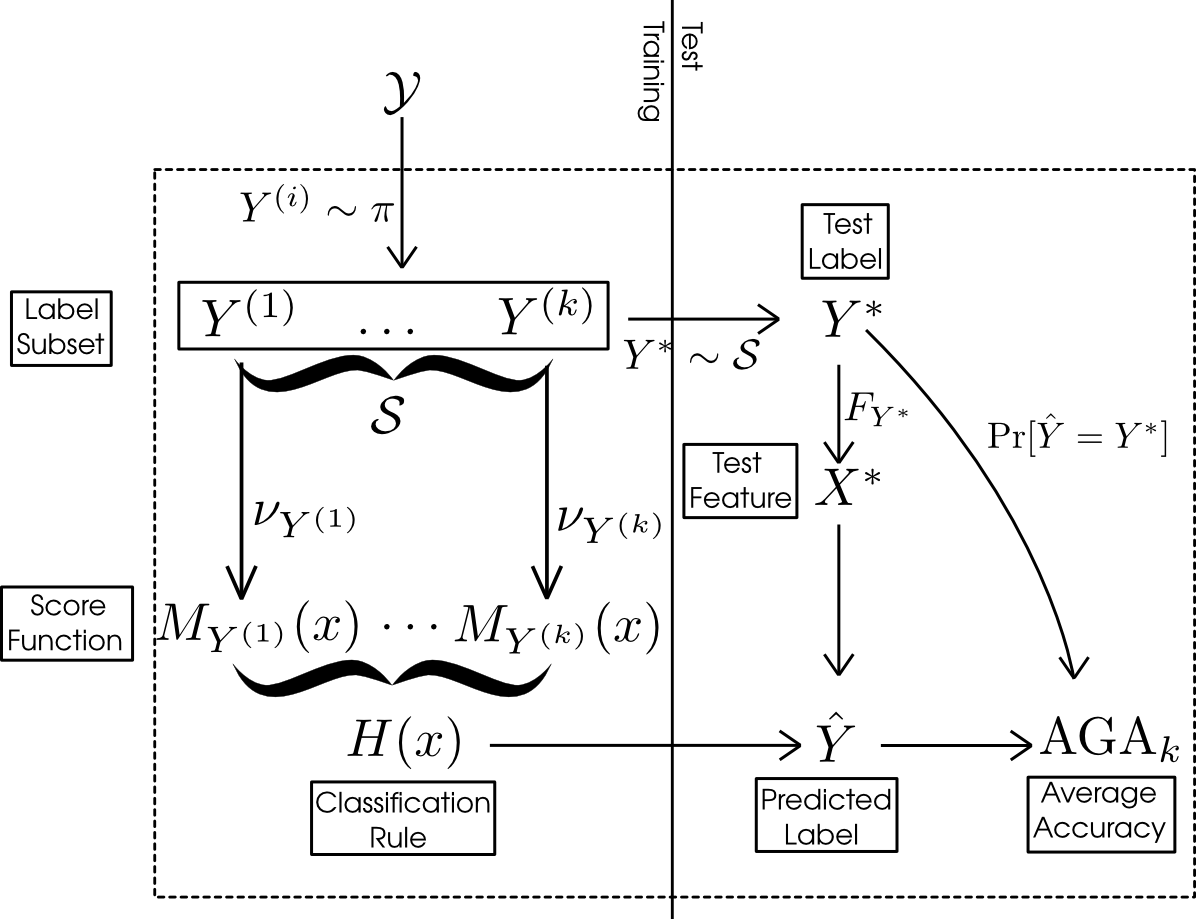
\includegraphics[scale = 0.3]{../extrapolation_simple/average_risk.png}
\caption{Average risk}\label{fig:average_risk2}
\end{figure}

\fi

As we can see from Figure \ref{fig:average_risk}, the average accuracy is
obtained by averaging over four randomizations:
\begin{enumerate}
\item[A1.] Drawing the label subset $\mathcal{S}$.
\item[A2.] Drawing the training dataset, $\hat{F}_{Y^{(1)}},\hdots, \hat{F}_{Y^{k}}.$
\item[A3.] Drawing $Y^*$ uniformly at random from $\mathcal{S}$.
\item[A4.] Drawing $X^*$ from $F_{Y^*}$.
\end{enumerate}


Our strategy is to analyze the average accuracy by
means of \emph{conditioning on} the true label and its training
sample, $(y^*, \hat{F}_{y^*})$, and the test feature $x^*$
while \emph{averaging} over all the other random variables.  Define
the \emph{conditional accuracy} $\text{CondAcc}_k((y^*, \hat{F}_{y^*}), x^*)$ as
\[
\text{CondAcc}_k((y^*, \hat{F}_{y^*}), x^*) = \Pr[\argmax_{y \in \mathcal{S}} \mathcal{M}(\hat{F}_y)(X^*) = Y^* |Y^*=y^*, X^* = x^*, \hat{F}_{Y^*} = \hat{F}_{y^*}].
\]
Figure \ref{fig:conditional_risk} illustrates the variables which are
fixed under conditioning and the variables which are randomized.
Compare to figure \ref{fig:average_risk}.

Without loss of generality, we can write the label subset $\mathcal{S}
= \{Y^*, Y^{(1)},\hdots, Y^{(k-1)}\}$.  Note that due to independence,
$Y^{(1)},\hdots, Y^{(k-1)}$ are still i.i.d. from $\pi$ even
conditioning on $Y^* = y^*.$ Therefore, the conditional risk can be
obtained via the following alternative order of randomizations:
\begin{enumerate}
\item[C0.] 
Fix $y^*, \hat{F}_{y^*},$ and $x^*$.  Note that $M_{y^*}(x^*)
= \mathcal{M}(\hat{F}_{y^*})(x^*)$ is also fixed.
\item[C1.]
Draw the \emph{incorrect labels} $Y^{(1)},\hdots, Y^{(k-1)}$ i.i.d. from
$\pi$.  (Note that $Y^{(i)} \neq y^*$ with probability 1 due to the
continuity assumptions on $\mathcal{Y}$ and $\pi$.)
\item[C2.]
Draw the training samples for the incorrect labels
$\hat{F}_{Y^{(1)}},\hdots, \hat{F}_{Y^{(k-1)}}$.  This determines
\[
\hat{Y} = \argmax_{y \in \mathcal{S}} M_y(x^*)
\]
and hence, whether or not the classification is correct for $(x^*, y^*)$
\end{enumerate}
Compared to four randomization steps for the average risk, we have
essentially conditioned on steps A3 and A4 and randomized over steps
A1 and A2.

\begin{figure}[h]
\centering
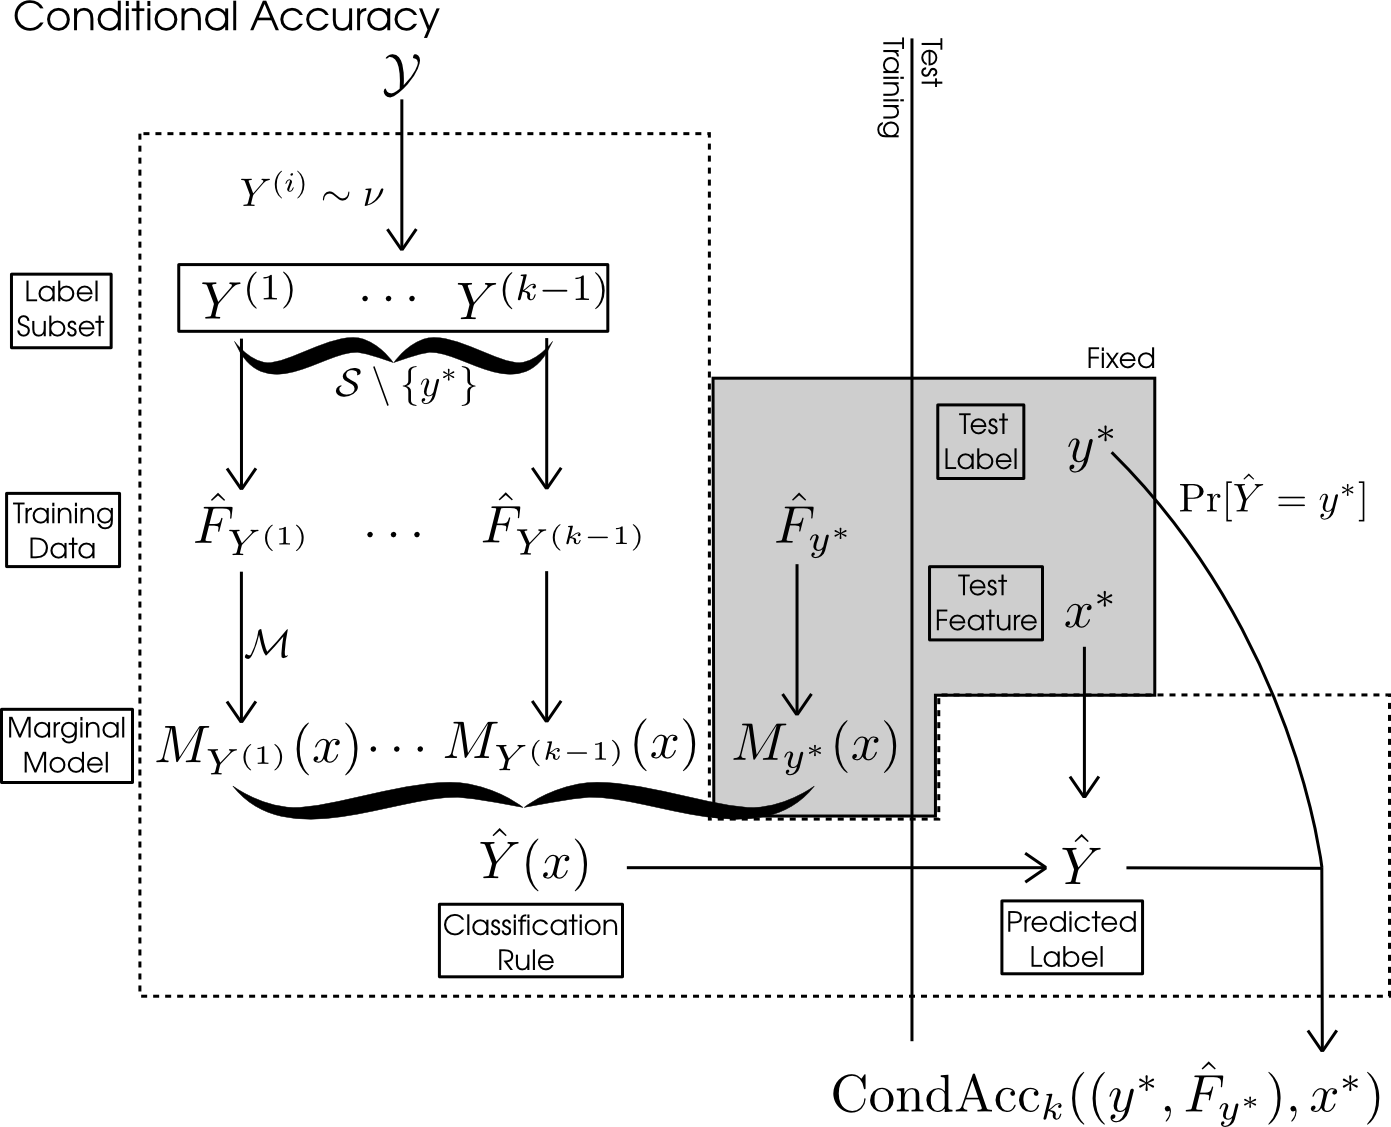
\includegraphics[scale = 0.3]{../extrapolation_simple/conditional_risk.png}
\caption{Conditional accuracy}\label{fig:conditional_risk}
\end{figure}

Now, in order to analyze the $k$-class behavior of the conditional
accuracy, we begin by considering the \emph{two-class} situation.

In the two-class situation, we have a true label $y^*$, a training
sample $\hat{F}_{y^*}$, and one incorrect label, $Y$.  
In this case, we obtain the margin functions for both classes from the training data,
\[
M_{y^*} = \mathcal{M}(\hat{F}_{y^*}),
\]
for the correct label,
and
\[
M_Y = \mathcal{M}(\hat{F}_Y)
\]
for the random incorrect label.  The classification is correct if and
only if \[M_{y^*}(x^*) \geq M_Y(x^*),\] that is, if the score of the
incorrect class is larger than the score of the correct class for
observation $x^*$.

Define the \emph{U-function} $U_{x^*}(y^*, \hat{F}_{y^*})$ as the
conditional accuracy (the probability of correct classification) in
the two-class case.  Since we are fixing $x^*$ and $(y^*,
\hat{F}_{y^*})$, the probability of correct classification is obtained
by taking an expectation:
\begin{align}\label{eq:U_function}
U_{x^*}(y^*, \hat{F}_{y^*}) &= \Pr[M_{y^*}(x^*) > \mathcal{M}(\hat{F}_Y)(x^*)]
\\&= \int_{\mathcal{Y} \times \mathcal{P}_{\mathcal{Y}}} 
I\{
M_{y^*}(x^*) > \mathcal{M}(\hat{F}_{y})(x^*)
\}
d\Pi_{y, r}(\hat{F}_y)
d\pi(y).
\end{align}
Recall that $\Pi_{y,r}$ is the distribution of $\hat{F}_y$, where
$\hat{F}_y$ is the empirical distribution of a sample of size $r$ from
label $y$ (that is, $\Pi_{y,r}$ is a distribution over distributions), as we defined in section 2.2.3.
See also figure \ref{fig:U_function} for an graphical illustration of
the definition.

\begin{figure}[h]
\centering
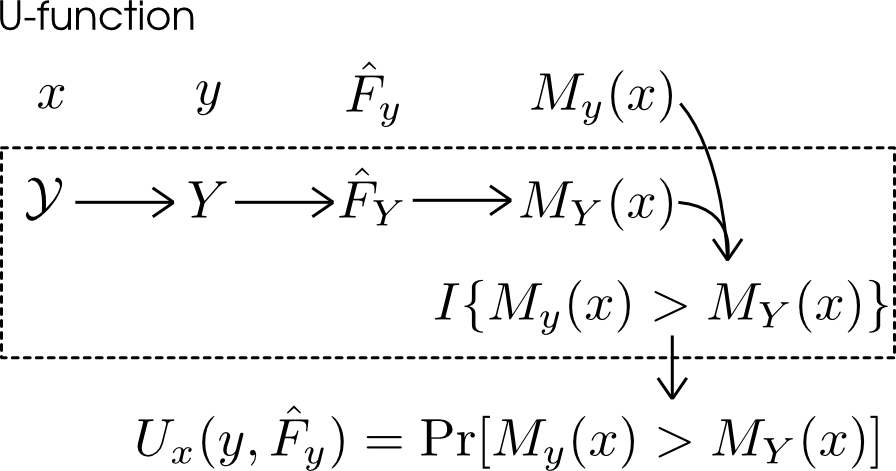
\includegraphics[scale = 0.4]{../extrapolation_figures/U_function.png}
\caption{U-functions}\label{fig:U_function}
\end{figure}

An important property of the U-function, and the basis for its name,
is that the random variable $U_X(Y, \hat{F}_Y)$ for $Y \sim \pi$ and
$\hat{F}_Y \sim \Pi_{Y, r}$ and $X \sim F_Y$, is uniformly distributed
conditional on $X=x$, for all fixed $x \in \mathcal{X}$.  This is
proved in the following Lemma.

\begin{lemma}\label{lemma:U_function}
Suppose $\pi$, $\{F_y\}_{y \in \mathcal{Y}}$ and marginal classifier
$\mathcal{F}$ satisfy the tie-breaking condition.  Take $x \in \mathcal{X}$.  Defining
$U_{y,\hat{F}_y}(x)$ as in \eqref{eq:U_function}, and defining the
random variable $U$ by
\[U = U_{Y, \hat{F}_Y}(X)\]
for $Y \sim \pi$, $\hat{F}_Y \sim \Pi_{Y, r}$ and $X \sim F_Y$.  Then
the conditional distribution of $U$ given $X = x$ for any $x \in
\mathcal{X}$ is uniform on $[0,1]$, i.e.
\[
\Pr[U \leq u|X =x] = \text{min}\{u, 1\}.
\]
\end{lemma}

\textbf{Proof of Lemma.}

%Define the variable $Z = \mathcal{M}(\hat{F}_Y)(x)$ for $Y \sim \pi$.
%By the tie-breaking condition, $Z$ has a continuous density on $[0,1]$.
%Consider the survivor function of $Z$, $g(z) = \Pr[Z \geq z]$.  From
%the definition \eqref{eq:U_function}, we see that 
%\[
%U = g(\mathcal{M}(\hat{F}_Y)(x)) = g(Z).
%\]
%Now note that the survivor function of any continuous random variable,
%when applied to itself, is uniformly distributed.

The result follows from the fact that the conditional probability
$\Pr[W > W'|W]$ is uniformly distributed for any $W, W'$ which are
i.i.d. with a continuous distribution.  

Define $Z = \mathcal{M}(\hat{F}_{Y})(x)$ and $Z' =
\mathcal{M}(\hat{F}_{Y'})(x)$ for $Y, Y' \stackrel{i.i.d.}{\sim} \pi$.
Then, conditional on $X = x$, we have
\[
U = \Pr[Z > Z'|Z].
\]
The tie-breaking conditional implies that $Z$ has a continuous
distribution, so therefore $U$ is uniformly distributed conditional on
$X = x$.  $\Box$


Now, we will see how the U-function allows us to understand the
$k$-class case.  Suppose we have true label $y^*$ and incorrect labels
$Y^{(1)},\hdots, Y^{(k-1)}$.  Note that the U-function
$U_{x^*}(y, \hat{F}_y)$ is monotonic in $M_y(x^*)$.  Therefore,
\[
\hat{Y} = \argmax_{y \in \mathcal{S}} M_y(x^*) = \argmax_{y \in \mathcal{S}} U_{x^*}(y, \hat{F}_y).
\]
Therefore, we have a correct classification if and only if the U-function value for the correct label
is greater than the maximum U-function values for the incorrect labels:
\[
\Pr[\hat{Y} = y^*] = \Pr[U_{x^*}(y^*, \hat{F}_{y^*}) > \max_{i=1}^{k-1} U_{x^*}(Y^{(i)}, \hat{F}_{Y^{(i)}})] =  \Pr[u^* > U_{max}].
\]
where $u^* = U_{x^*}(y^*, \hat{F}_{y^*})$ and $U_{max, k-1}
= \max_{i=1}^{k-1} U_{x^*}(Y^{(i)}, \hat{F}_{Y^{(i)}})$.  But now,
observe that we know the distribution of $U_{max, k-1}$.  Since
$U_{x^*}(Y^{(i)}, \hat{F}_{Y^{(i)}})$ are i.i.d. uniform, we know that
\begin{equation}\label{eq:umax_beta}
U_{max, k-1} \sim \text{Beta}(k-1, 1). 
\end{equation}

Therefore, in the general case, the conditional accuracy is
\[
\text{CondAcc}_k((y^*, \hat{F}_{y^*}), x^*) = \Pr[U_{max} \leq u^*] = \int_0^{u^*} (k-1) u^{k-2} du.
\]
Now the average accuracy can be obtained by integrating over the
distribution of $U^* = U_{X^*}(Y^*, \hat{F}_{Y^*})$, which we state in
the following proof of theorem \ref{theorem:avrisk_identity}.

\noindent\textbf{Proof of Theorem \ref{theorem:avrisk_identity}}.
We have
\begin{align*}
\text{AGA}_{k,r} &= \E[\int_0^{U^*} (k-1) u^{k-2} du] 
\\&= \E[\int_0^1 I\{u \leq U^*\} (k-1) u^{k-2} du ]
\\&= (k-1) \int_0^1 \Pr[U^* \geq u] u^{k-2} du.
\end{align*}
Or equivalently,
\[
\text{AGA}_{k, r}((y^*, \hat{F}_{y^*}), x^*) = 1 - (k-1) \int \bar{D}(u) u^{k-2} du.
\]
where $\bar{D}(u)$ denotes the cumulative distribution function of $U^*$ on $[0,1]$:
\begin{equation}\label{eq:Kbar}
\bar{D}(u) = \Pr[U_{X^*}(Y^*, \hat{F}_{y^*}) \leq u].
\end{equation}
We have expressed the average risk expressed as a weighted integral of
a certain function $\bar{D}(u)$ defined on $u \in [0,1]$.  We have
clearly isolated the part of the average risk which is independent of
$k$--the univariate function $\bar{D}(u)$, and the part which is
dependent on $k$--which is the density of $U_{max}$.

In section \ref{sec:extrapolation_estimation}, we will develop
estimators of $\bar{D}(u)$ in order to estimate the $k$-class average
risk.

Having this theoretical result allows us to understand how the
expected $k$-class risk scales with $k$ in problems where all the
relevant densities are known.  However, applying this result in
practice to estimate $\text{AGA}_k$ requires some means of
estimating the unknown function $\bar{D}$--which we discuss in the
following.

\section{Estimation}\label{sec:extrapolation_estimation}

Now we address the problem of estimating $\text{AGA}_{k_2, r_1}$ from
data.  As we have seen from Theorem \ref{theorem:avrisk_identity}, the
$k$-class average accuracy of a marginal classifier $\mathcal{M}$ is a
functional of a object called $\bar{D}(u),$ which depends marginal
model $\mathcal{M}$ of the classifier, the joint distribution of
labels $Y$ and features $X$ when $Y$ is drawn from the population
density $\pi$.

Therefore, the strategy we take is to attempt to estimate $\bar{D}$
for the given classification model, and then plug in our estimate of
$\bar{D}$ into the integral \eqref{eq:avrisk_identity} to obtain an
estimate of $\text{AGA}_{k_2, r_{train}}$.

Having decided to estimate $\bar{D}$, there is then the question of
what kind of model we should assume for $\bar{D}$.  In this work, we
assume that some parametric model\footnote{While a
nonparametric approach may be more ideal, we leave this to future work.} is available for $\bar{D}$.

Let us assume the linear model
\begin{equation}\label{eq:linearKu}
\bar{D}(u) = \sum_{\ell = 1}^m \beta_\ell h_\ell(u),
\end{equation}
where $h_\ell(u)$ are known basis functions, and $\beta$ are the model
parameters to be estimated. We can obtain \emph{unbiased} estimation
of $\text{AGA}_{k_2, r_{train}}$ via the unbiased estimates of
$k$-class average risk obtained from \eqref{eq:avtestrisk}.

If we plug in the assumed linear model \eqref{eq:linearKu} into the
identity \eqref{eq:avrisk_identity}, then we get
\begin{align}
1 - \text{AGA}_{k, r_{train}} &= (k-1)\int \bar{D}(u) u^{k-2} du
\\&= (k-1)\int_0^1 \sum_{\ell = 1}^m \beta_\ell h_\ell(u) u^{k-2} du
\\&= \sum_{\ell = 1}^m \beta_\ell H_{\ell,k} \label{eq:avrisk_linear}
\end{align}
where
\begin{equation}
H_{\ell,k} = (k-1) \int_0^1 h_\ell(u) u^{k-2} du.
\end{equation}
The constants $H_{\ell, k}$ are moments of the basis function
$h_\ell$: hence we call this method the \emph{moment method.}  Note
that $H_{\ell, k}$ can be precomputed numerically for any $k \geq 2$.


Now, since the test accuracies $\text{TA}_k$ are unbiased estimates of
$\text{AGA}_{k, r_{train}}$, this implies that the regression
estimate
\[
\hat{\beta} = \argmin_\beta \sum_{k=2}^{k_1} \left( (1 - \text{TA}_k) - \sum_{\ell=1}^m \beta_\ell H_{\ell, k}\right)^2
\]
is unbiased for $\beta$.
The estimate of $\text{AGA}_{k_2,r_1}$ is similarly obtained
from \eqref{eq:avrisk_linear}, via
\begin{equation}\label{eq:avrisk_hat}
\widehat{\text{AGA}_{k_2,r_1}} = 1 - \sum_{\ell=1}^m \hat{\beta}_\ell H_{\ell, k_2}.
\end{equation}

We have not discussed how to choose the basis functions $\{h_\ell\}$ in practice,
nor what kind of additional constraints can be imposed on the estimation to improve performance.
While these are important practical issues, we leave these questions to future work.
However, we will see some of these considerations at play in the next section,
when we apply the estimation method to a real-data example.

\section{Examples}\label{sec:extrapolation_example}

\subsection{Facial recognition example}

From the ``Labeled Faces in the Wild'' dataset (\cite{LFWTech}), we
selected 1672 individuals with at least 2 face photos.  We form a
dataset consisting of photo-label pairs $(\vec{z}_j^{(i)}, y^{(i)})$
for $i = 1,\hdots, 1672$ and $j = 1,2$ by randomly selecting 2 face
photos for each of the 1672 individuals.

We implement a face recognition system based on one nearest-neighbor
and OpenFace (\cite{amos2016openface}) for feature extraction.  For
each photo $\vec{z}$, a 128-dimensional feature vector $\vec{x}$ is
obtained as follows.
\begin{enumerate}
\item The computer vision library DLLib is used to detect landmarks in
  $\vec{z}$, and to apply a nonlinear transformation to align
  $\vec{z}$ to a template.
\item The aligned photograph is downsampled to a $96 \times 96$ input,
  which is fed into a pre-trained deep convolutional neural network to
  obtain the 128-dimensional feature vector $\vec{x}$.
\end{enumerate}
Therefore, we obtain feature-label pairs $(\vec{x}_j^{(i)}, y^{(i)})$
for $i = 1,\hdots, 1672$ and $j = 1,2$.

The recognition system then works as follows.  Suppose we want to
perform facial recognition on a subset of the individuals, $I \subset
\{1,\hdots, 1672\}$.  Then, for all $i \in I$, we load one feature
vector-label pair, into the system, $(\vec{x}_1^{(i)}, y^{(i)})$.  In
order to identify a new photo $\vec{z}^*$, we obtain the feature
vector $\vec{x}^*$, and guess the label $\hat{y}$ based on example
with the minimal distance to $\vec{x}^*$,
\[
\hat{y} = y^{(i^*)}
\]
where
\[
i^* = \text{argmin}_i d(\vec{x}, \vec{x}_1^{(i)}).
\]
The test accuracy is assessed on the unused repeat for all individuals
in $I$.  Note that the assumptions of our estimation method are met in
this example because one-nearest neighbor is a marginal classifier.
One can define the margin functions as
\[
(\mathcal{M}(\vec{x}))(\vec{x}^*) = -||\vec{x} - \vec{x}^*||^2.
\]
We note that $m$-nearest neighbor for $m > 1$ is not marginal.

While we can apply our extrapolation method to estimate the average
accuracy for any number of faces $k$, it will not be possible to
validate our estimates if we use the full dataset.  Therefore, we take
the average accuracies computed using the subsampling method
\eqref{eq:avtestrisk} on the full dataset as a \emph{ground truth} to
compare to the average accuracy estimated from a \emph{subsampled}
dataset.  Therefore, we simulate the problem of performance
extrapolation from a database of $K$ faces by subsampling a
dataset of size $K$ from the LFW dataset.

\begin{figure}
\centering
\begin{tabular}{cc}
a & b\\
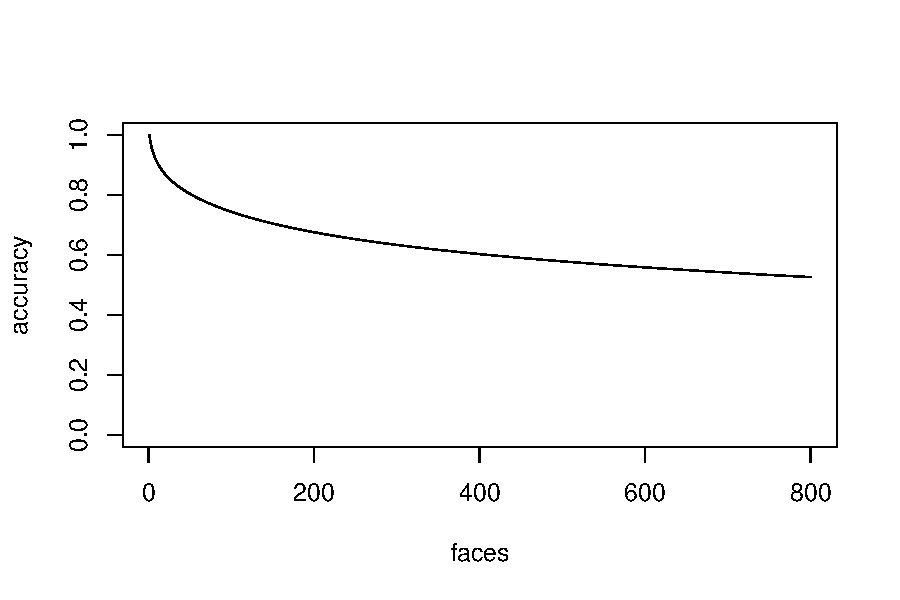
\includegraphics[height = 3in]{../../facerec/acc_plot1.pdf} &
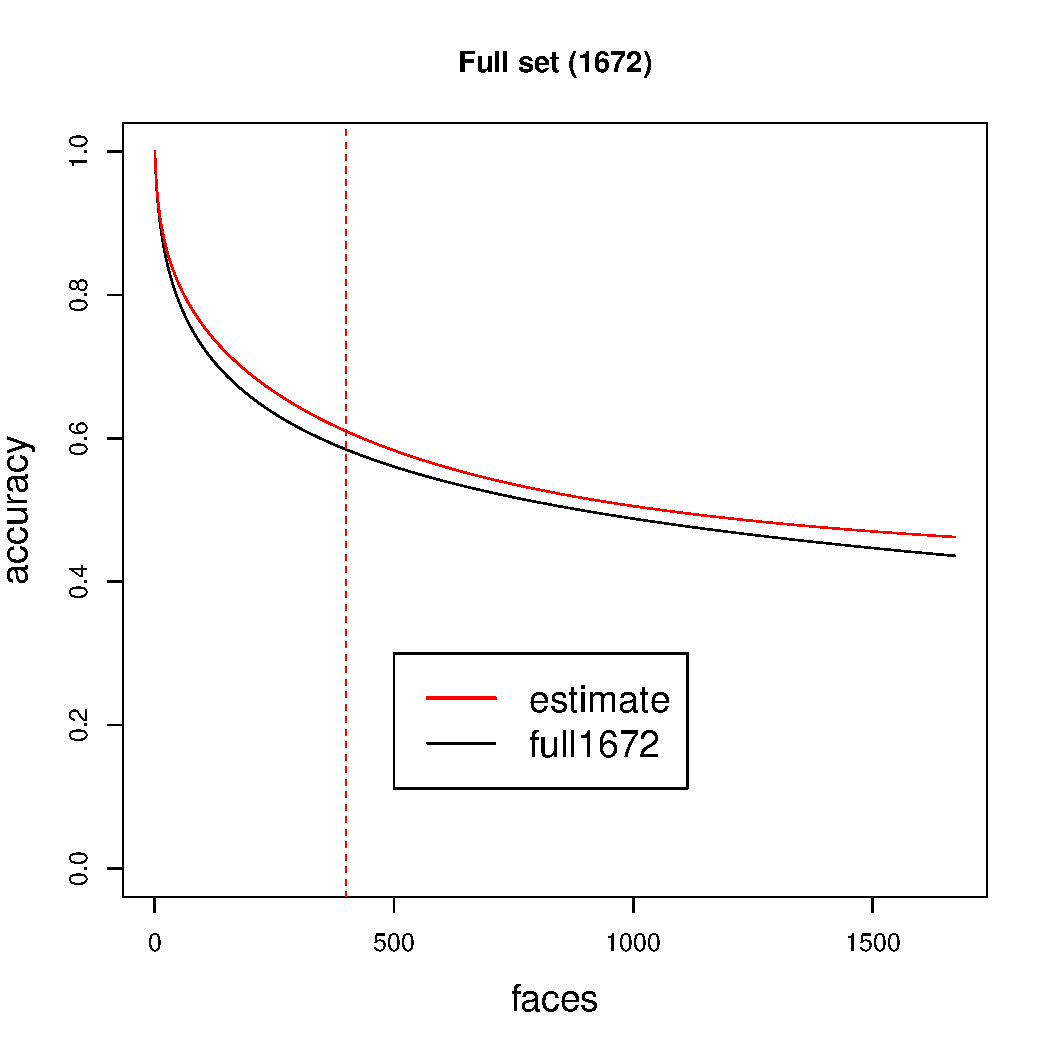
\includegraphics[height = 3in]{../../facerec/acc_plot2.pdf}
\end{tabular}
\caption{(a) The estimated average accuracy for $k = 2,\hdots,
  400$ given a dataset of 400 faces subsampled from Labeled Faces in
  the Wild.  (b) Estimated average accuracy for $k > 400$ on the
  same dataset, compared to the ground truth (average $k$-class test accuracy
  using all 1672 classes).}
\label{fig:lfw_extrapolation1}
\end{figure}

To do the performance extrapolation, we use a linear
spline basis,
\[
h_\ell(u) = \left[u - \frac{\ell - 1}{m}\right]_+
\]
for $\ell = 1,\hdots, m$.  Here we take $m = 10000$.  We model the
function $\bar{D}(u)$ as a non-negative linear combination of basis
functions,
\[
\bar{D}(u) = \sum_{\ell = 1}^m \beta_\ell h_\ell(u),
\]
with $\beta_\ell \geq 0$.  The non-negativity constraint on the
coefficients $\beta$, combined with the linear spline basis, ensures
that $\bar{D}(u)$ is a monotonic and convex function on $[0,1]$.  We
have found that in many simulated examples, $D(u)$ appears to be
monotone and convex, and we have also found that including the
monotonicity and convexity constraint in the estimation procedure
improves performance in practical examples.  The resulting estimated
generalization accuracies, computed using \eqref{eq:avrisk_identity},
are plotted in Figure \eqref{fig:lfw_extrapolation1} (b).  As we
already mentioned, to assess the quality of the estimated average
accuracy, we compare them to the `ground truth' accuracy curve
obtained by using all 1672 examples to compute the the average test
risk.



To get an idea of the accuracy and variance of the accuracy curve
estimates for varying sample sizes $K$, we repeat this procedure
multiple times for $K \in \{100,200,400, 800\}$.  The results, again
compared to the ground truth computed from the full data set, are
illustrated in figure \ref{fig:lfw_extrapolation2}.

\begin{figure}
\centering
\begin{tabular}{cc}
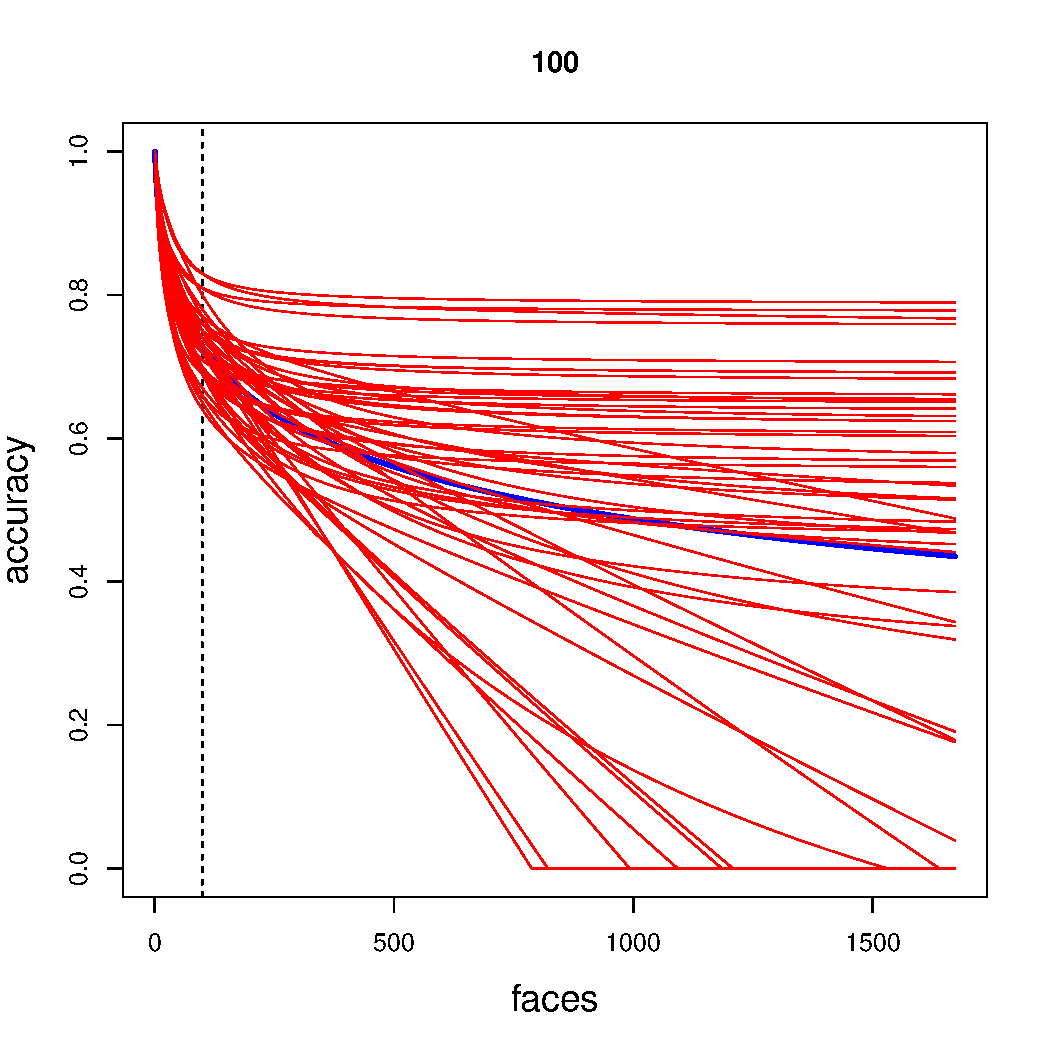
\includegraphics[scale = 0.4]{../../facerec/sub_100.pdf} &
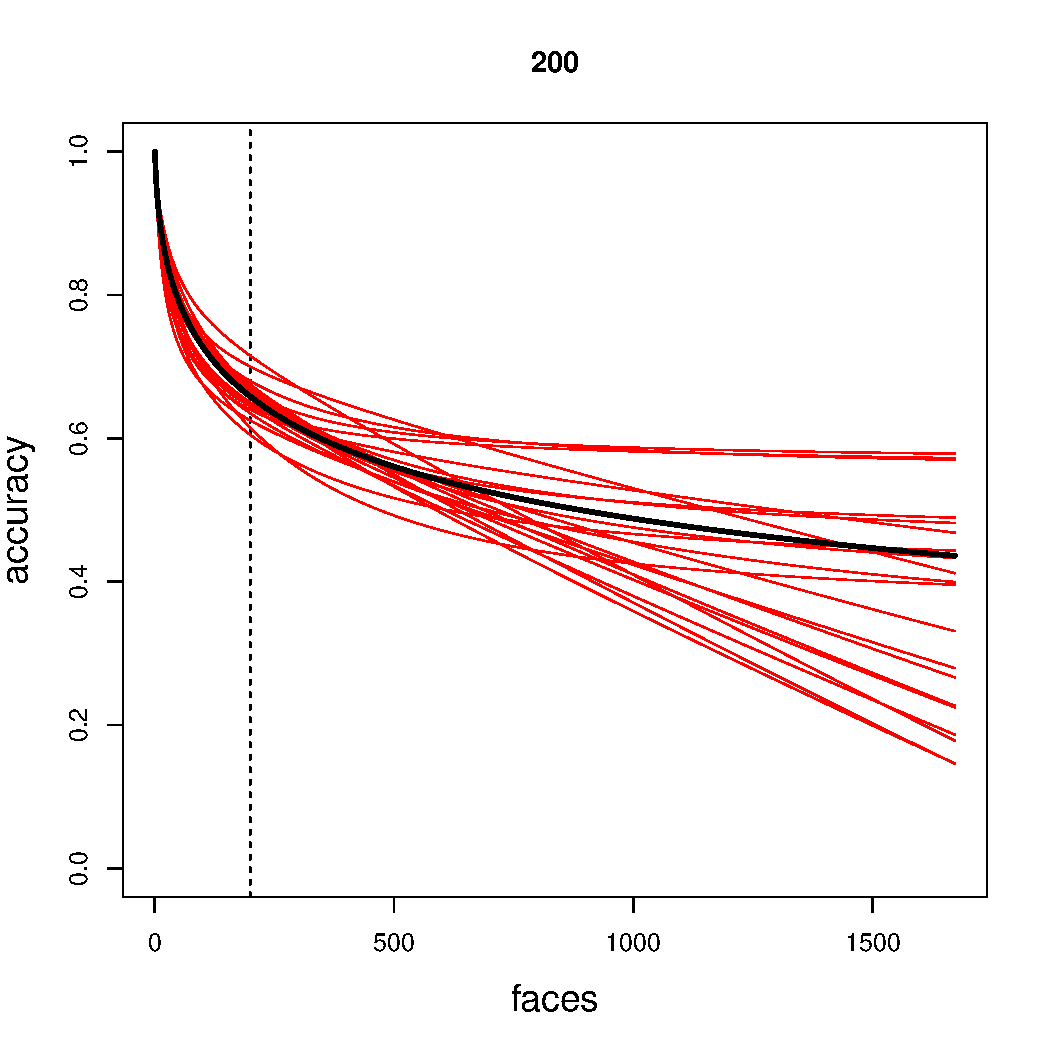
\includegraphics[scale = 0.4]{../../facerec/sub_200.pdf} \\
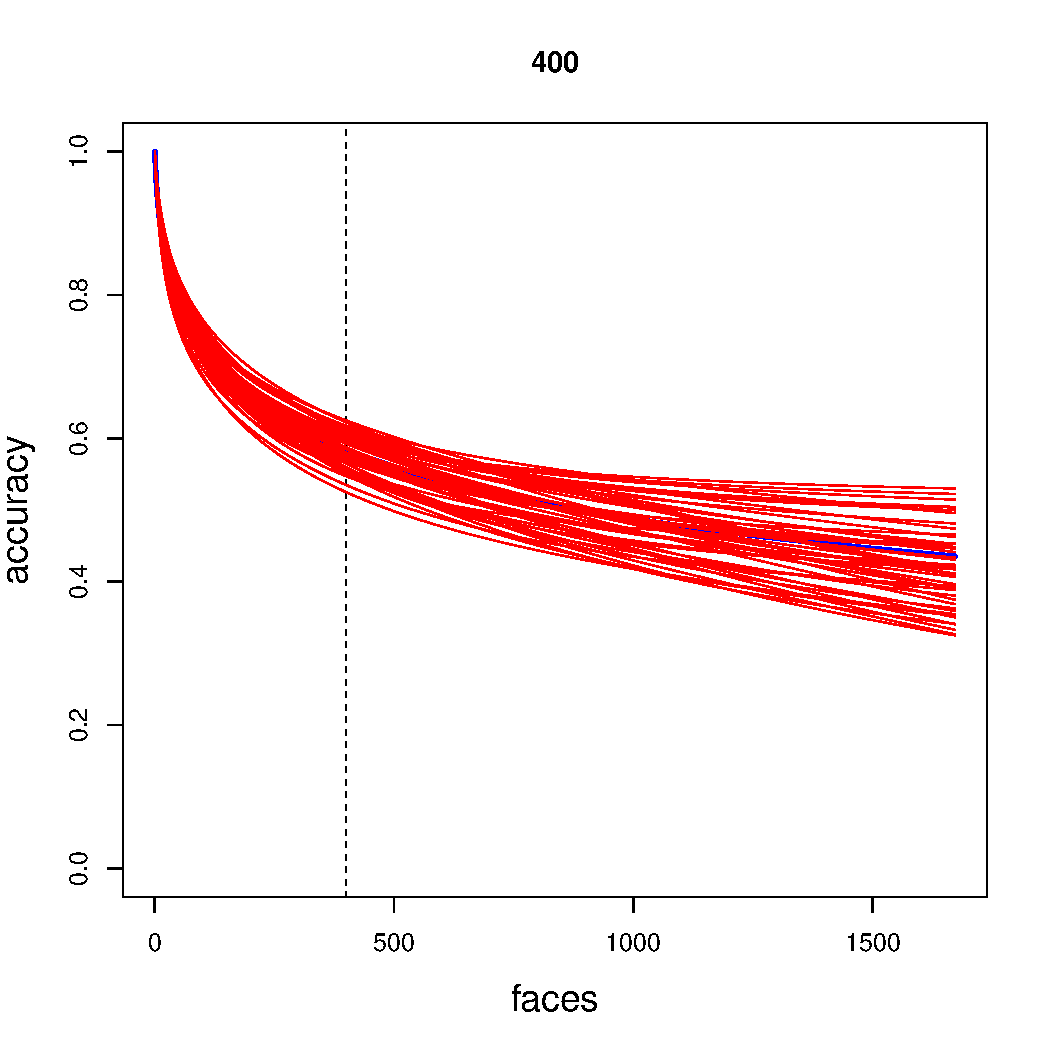
\includegraphics[scale = 0.4]{../../facerec/sub_400.pdf} &
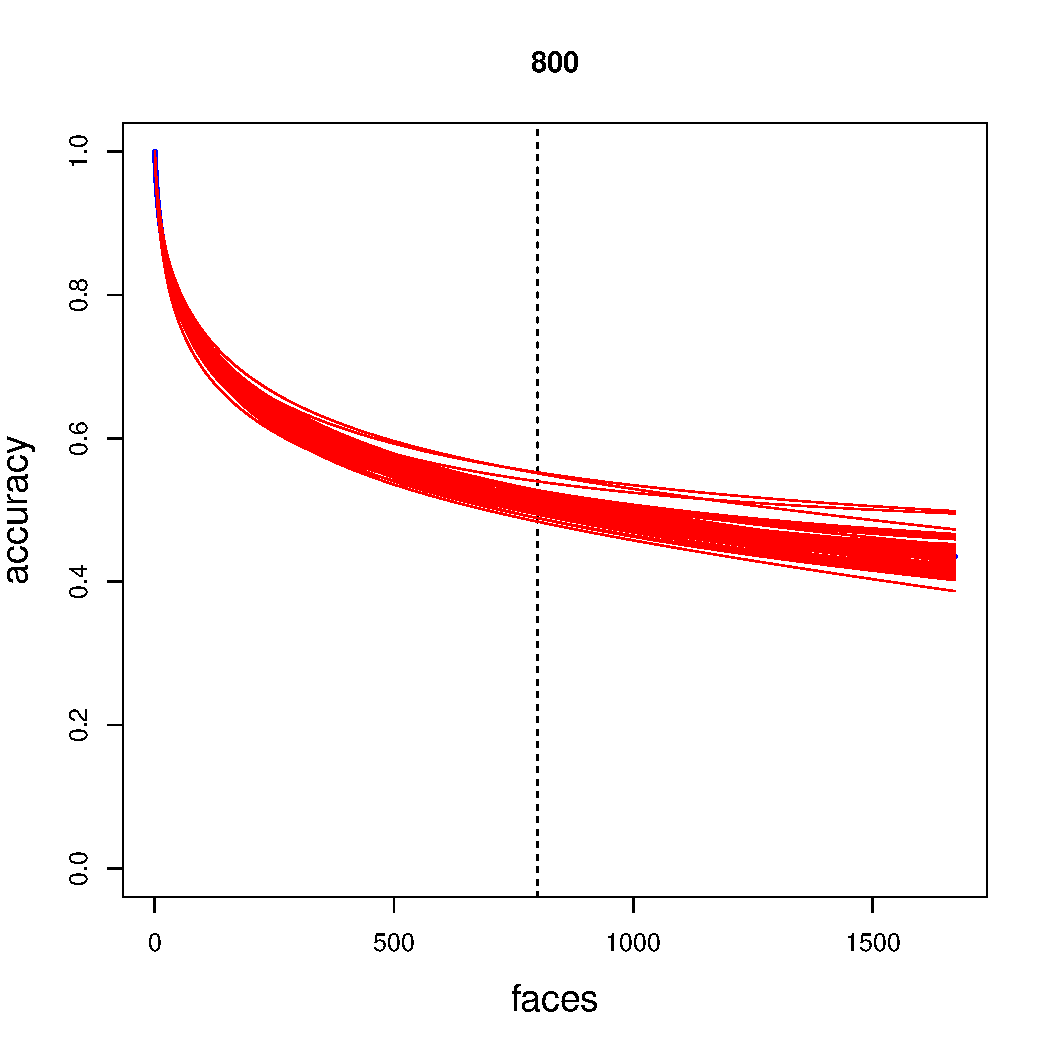
\includegraphics[scale = 0.4]{../../facerec/sub_800.pdf} 
\end{tabular}
\caption{Estimated average accuracy using subsampled datasets of size
  $k$, compared to the ground truth (average $k$-class test accuracy
  using all 1672 classes).}
\label{fig:lfw_extrapolation2}
\end{figure}

\subsection{Telugu OCR example}

While the previous example was a perfect fit to the assumptions of the
framework, we also want to see how well the method works when some of
the assumptions may be violated.  Towards this end we apply performance
extrapolation in an optical character recognition example
(\cite{achanta2015telugu}) for predicting the accuracy on 400 classes
of Telugu characters from a subsample of size $K = 20$.  We consider
the use of five different classifiers: Naive Bayes, logistic
regression, SVM, $\epsilon$-nearest neighbors\footnote{$m$-nearest
  neighbors with $m = \epsilon n$ for fixed $\epsilon > 0$}, and a
deep convolutional neural network\footnote{The network architecture is
  as follows: {\tt
    48x48-4C3-MP2-6C3-8C3-MP2-32C3-50C3-MP2-200C3-SM.}}.  Of the five
classifiers, only Naive Bayes satisfies the marginal classifier
assumption.  Again, we compare the result of our model to the ground
truth obtained by using the full dataset.

\begin{table}
\centering
\begin{tabular}{|c||c|c|c|}\hline
Classifier      & Test $\text{acc}^{(20)}$ & Test $\text{acc}^{(400)}$ & $\hat{AGA}_{400}$ \\ \hline
Naive Bayes     & 0.951                   & 0.601                   & 0.858     \\ \hline
Logistic        & 0.922                   & 0.711                   & 0.812     \\ \hline
SVM             & 0.860                   & 0.545                   & 0.687     \\ \hline
$\epsilon$-NN   & 0.951                   & 0.591                   & 0.410     \\ \hline
Deep neural net & 0.995                   & 0.986                   & 0.907     \\ \hline
\end{tabular}
\caption{Performance extrapolation: predicting the accuracy on 400 classes using data from 20 classes on a Telugu character dataset.
$\epsilon = 0.002$ for $\epsilon$-nearest neighbors.}
\label{tab:telugu}
\end{table}

The results are displayed in Table \ref{tab:telugu}.  To our surprise,
the worst absolute difference between ground truth and estimated
average accuracy was in the case of Naive Bayes $(|\delta| = 0.257)$
which satisfies the marginal property.  All other classifiers had
absolute errors less than 0.2.  It is also interesting to note that,
even though Naive Bayes and $\epsilon$-nearest neighbors have the same
test accuracy on the subset, that the predicted accuracy on 400
differs greatly between then (0.858 vs 0.400).
%Furthermore, the
%difference is in the right direction: Naive Bayes is predicted to work
%better on 400 classes than $\epsilon$-nearest neighbors, which appears
%to be the case based on the 400-class test accuracy.

While further work is still needed to better understand the
performance of the proposed performance extrapolation method, both for
marginal classifiers (which satisfy the theoretical assumptions) and
non-marginal classifiers (which do not), the results obtained in these
two examples are encouraging in the sense that useful predictions
were obtained both for marginal and non-marginal classifiers.

% Chapter 4

\chapter{Inference of mutual information} % Main chapter title

\label{Chapter4} % For referencing the chapter elsewhere, use \ref{Chapter1} 

\section{Motivation}

As we discussed in the introduction, the mutual information $I(X; Y)$
provides one method for the supervised evaluation of representations.
Recall that Shannon's mutual information $I(X; Y)$ is fundamentally a
measure of dependence between random variables $X$ and $Y$, defined as
\[
I(X;Y) = \int p(x, y) \log \frac{p(x, y)}{p(x)p(y)}dxdy.
\]
Various properties of $I(\vec{g}(\vec{Z}); Y)$, such as sensitivity to
nonlinear relationships, symmetry, and invariance to bijective
transformations, make it ideal for quantifying the information between
a representation of an input vector $\vec{g}(\vec{Z})$ and a response
$Y$ which is possible vector-valued.  However, current methods
estimating mutual information for high-dimensional data require large
and over-parameterized generative models.  For instance, one can
tractably estimate mutual information by assuming a multivariate
Gaussian model: however, this approach essentially assumes a linear
relationship between the input and output, and hence fails to quantify
nonlinear dependencies.  

Hence, a popular approach which combines the strengths of the machine
learning approach for modeling high-dimensional data and the
advantages of the information theoretic approach is to obtain a lower
bound on the mutual information by using the confusion matrix of a
classifier.  This is the most popular approach for estimating mutual
information in neuroimaging studies, but suffers from known
shortcomings (Gastpar 2010, Quiroga 2009).  The idea of linking
classification performance to mutual information dates back to the
beginnings of information theory: Shannon's original motivation was to
characterize the minimum achievable error probability of a noisy
communication channel.  More explicitly, Fano's inequality provides a
lower bound on mutual information in relation to the optimal
prediction error, or Bayes error.  Fano's inequality can be further
refined to obtain a tighter lower bound on mutual information (Tebbe
and Dwyer 1968.)  However, a shortcoming to the classification-based
approach is that it requires either for the response $Y$ to already be
discrete, or to discretize the response $Y$ into finitely many
classes.

In this paper, we develop an analogue of Fano's inequality for the
\emph{identification task}, rather than the classification task, which
can therefore be applied to the case of a continuous response $Y$.  In
this way, we derive a new machine-learning based estimator of mutual
information $I(X; Y)$ which can be applied without the need to
discretize a continuous response.

As we saw in Chapter 2, the identification task is highly related to
the randomized classification framework.  Therefore, we analyse the
identification risk by means of the $k$-class average Bayes accuracy,
which provides an upper bound to identification accuracy.  Our main
theoretical contributions are (i) the derivation of a tight lower
bound on mutual information as a function of $k$-class average Bayes
accuracy, and (ii) the derivation of an asymptotic relationship
between the $K$-class average Bayes accuracy and the mutual
information. Our method therefore estimates of the $K$-class Bayes
identification accuracy to be translated into estimate of the mutual
information.

The rest of the chapter is organized as follows.  Section
\ref{sec:ch4_theory} establishes the theoretical results linking
average Bayes accuracy and mutual information, and section
\ref{sec:ch4_estimation} describes our proposed identification-based
estimator of mutual information based on the theory.  We see some
examples of applications in the next chapter, where the estimator
developed here is compared to an alternative estimator, which is based
on high-dimensional asymptotics.

\section{Average Bayes accuracy and Mutual information}\label{sec:ch4_theory}

\subsection{Problem formulation and result}

Let $\mathcal{P}$ denote the collection of all joint densities $p(x,
y)$ on finite-dimensional Euclidean space.  For $\iota \in [0,\infty)$
define $C_k(\iota)$ to be the largest $k$-class average Bayes error
attained by any distribution $p(x,y)$ with mutual information not
exceeding $\iota$:
\[
C_k(\iota) = \sup_{p \in \mathcal{P}: \text{I}[p(x,y)] \leq \iota} \text{ABA}_k[p(x,y)].
\]
A priori, $C_k(\iota)$ exists since $\text{ABA}_k$ is bounded between
0 and 1.  Furthermore, $C_k$ is nondecreasing since the domain of the
supremum is monotonically increasing with $\iota$.

It follows that for any density $p(x,
y)$, we have
\[
\text{ABA}_k[p(x,y)] \leq C_k(\text{I}[p(x,y)]).
\]
Hence $C_k$ provides an upper bound for average Bayes error in terms of mutual information.

Conversely we have
\[
\text{I}[p(x,y)] \geq C^{-1}_k(\text{ABA}_k[p(x,y)])
\]
so that $C^{-1}_k$ provides a lower bound for mutual information in terms of average Bayes error.

On the other hand, there is no nontrivial \emph{lower} bound for average Bayes error in terms of mutual information,
nor upper bound for mutual information in terms of average Bayes error, since
\[
\inf_{p \in \mathcal{P}: \text{I}[p(x,y)] \leq \iota} \text{ABA}_k[p(x,y)] = \frac{1}{k}.
\]
regardless of $\iota$.

The goal of this work is to attempt to compute or approximate the functions $C_k$ and $C_k^{-1}$.

In the following sections we determine the value of $C_k(\iota)$,
leading to the following result.

\begin{theorem}\label{theorem:Cunif}
For any $\iota > 0$, there exists $c_\iota \geq 0$ such that defining
\[
Q_c(t) = \frac{\exp[ct^{k-1}]}{\int_0^1 \exp[ct^{k-1}]},
\]
we have
\[
\int_0^1 Q_{c_\iota}(t) \log Q_{c_\iota}(t) dt = \iota.
\]
Then,
\[
C_k(\iota) = \int_0^1 Q_{c_\iota}(t) t^{k-1} dt.
\]
\end{theorem}

We obtain this result by first reducing the problem to the case of
densities with uniform marginals, then doing the optimization over the
reduced space.

\subsection{Reduction}

Let $p(x, y)$ be a density supported on
$\mathcal{X} \times \mathcal{Y}$, where $\mathcal{X}$ is a subset of
$\mathbb{R}^{d_1}$ and $\mathcal{Y}$ is a subset of
$\mathbb{R}^{d_2}$, and such that $p(x)$ is uniform on $\mathcal{X}$
and $p(y)$ is uniform on $\mathcal{Y}$.

Now let $\mathcal{P}^{unif}$ denote the set of such distributions:
in other words, $\mathcal{P}^{unif}$ is the space of joint densities in Euclidean space
with uniform marginals over the marginal supports.
In this section, we prove that
\[
C_k(\iota) =\inf_{p \in \mathcal{P}: \text{I}[p(x,y)] \leq \iota} \text{ABA}_k[p(x,y)] = 
\inf_{p \in \mathcal{P}^{unif}: \text{I}[p(x,y)] \leq \iota} \text{ABA}_k[p(x,y)],
\]
thus reducing the problem of optimizing over the space of all
densities to the problem of optimizing over densities with uniform
marginals.

Also define $\mathcal{P}^{bounded}$ to be the space of all densities $p(x, y)$ with finite-volume support.
Since uniform distributions can only be defined over sets of finite volume, we have
\[
\mathcal{P}^{unif} \subset \mathcal{P}^{bounded} \subset \mathcal{P}.
\]

Therefore, it is necessary to first show that
\[
\inf_{p \in \mathcal{P}: \text{I}[p(x,y)] \leq \iota} \text{ABA}_k[p(x,y)] = 
\inf_{p \in \mathcal{P}^{bounded}: \text{I}[p(x,y)] \leq \iota} \text{ABA}_k[p(x,y)].
\]

This is accomplished via the following lemma.

\begin{lemma}\label{lemma:truncation} (Truncation).
Let $p(x, y)$ be a density on
$\mathbb{R}^{d_x} \times \mathbb{R}^{d_y}$.  For all $\epsilon > 0$,
there exists a subset $\mathcal{X} \subset \mathbb{R}^{d_x}$ with
finite volume with respect to $d_x$-dimensional Lesbegue measure, and
a subset $\mathcal{Y} \subset \mathbb{R}^{d_y}$ with finite volume
with respect to $d_y$-dimensional Lesbegue measure, such that defining
\[
\tilde{p}(x, y) = \frac{I\{(x,y) \in \mathcal{X}\times \mathcal{Y}\} }{\int_{\mathcal{X} \times \mathcal{Y}} p(x,y) dx dy} p(x,y),
\]
we have
\[
|\text{I}[p] - \text{I}[\tilde{p}]| < \epsilon
\]
and
\[
|\text{ABA}_k[p] - \text{ABA}_k[\tilde{p}]| < \epsilon.
\]
\end{lemma}

\textbf{Proof.}
Recall the definition of the Shannon entropy $H$:
\[
\text{H}[p(x)] = - \int p(x) \log p(x) dx.
\]
It is a well-known in information theory that
\[
\text{I}[p(x, y)] = \text{H}[p(x)] + \text{H}[p(y)] - \text{H}[p(x, y)].
\]
There exists a sequence $(\mathcal{X}_i, \mathcal{Y}_i)_{i=1}^\infty$
where $(\mathcal{X}_i)_{i=1}^\infty$ is an increasing sequence of finite-volume subsets of $\mathbb{R}^{d_x}$
and $(\mathcal{Y}_i)_{i=1}^\infty$ is an increasing sequence of finite-volume subsets of $\mathbb{R}^{d_y}$,
and $\lim_{i \to \infty} \mathcal{X}_i = \mathbb{R}^{d_x}$, $\lim_{i \to \infty} \mathcal{Y}_j$.
Define
\[
\tilde{p}_i(x, y) = \frac{I\{(x,y) \in \mathcal{X}_i\times \mathcal{Y}_i\} }{\int_{\mathcal{X}_i \times \mathcal{Y}_i} p(x,y) dx dy} p(x,y)
\]
Note that $\tilde{p}_i$ gives the conditional distribution of $(X, Y)$
conditional on $(X, Y) \in \mathcal{X}_i \times \mathcal{Y}_i$. 
Furthermore, it is convenient to define $\tilde{p}_\infty = p$.
We can find some $i_1$, such that for all $i \geq i_1$, we have
\[
\left|\int_{x \notin \mathcal{X}_i} p(x) \log p(x) dx\right| < \frac{\epsilon}{6}
\]
\[
\left|\int_{y \notin \mathcal{Y}_i} p(y) \log p(y) dy\right| < \frac{\epsilon}{6}
\]
\[
\left|\int_{(x,y) \notin \mathcal{X}_i \times \mathcal{Y}_i} p(x, y) \log p(x, y) dx dy\right| < \frac{\epsilon}{6}
\]
and also such that
\[
-\log \left[\int_{x, y \in \mathcal{X}_i \times \mathcal{Y}_i} p(x, y) dx dy\right] < \frac{\epsilon}{2}
\]
Then, it follows that
\[
|\text{I}[p] - \text{I}[\tilde{p}_i]| < \epsilon
\]
for all $i \geq i_1$.

Now we turn to the analysis of average Bayes error.
Let $f_i$ denote the Bayes $k$-class classifier for $\tilde{p}_i(x, y)$
and
$f_\infty$ the Bayes $k$-class classifier for $p(x, y)$: recall that by definition,
\[
\text{ABA}_k[\tilde{p}_i] = \Pr_{\tilde{p}_i}[f_i(X^{(1)},...,X^{(k)}, Y) = Z]
\]
Define
\[
\epsilon_i = \Pr_p[(X^{(1)},...,X^{(k)}, Y)\notin \mathcal{X}_i^k \times \mathcal{Y}_i];
\]
by continuity of probability we have $\lim_i \epsilon_i \to 0$.
We claim that
\[
|\text{ABA}_k[\tilde{p}_i] - \text{ABA}_k[p]| \leq \epsilon_i.
\]
Given the claim, the proof is completed by finding $i > i_1$ such that $\epsilon_i < \epsilon$,
and defining $\mathcal{X} = \mathcal{X}_i$, $\mathcal{Y} = \mathcal{Y}_i$.

Consider using $f_i$ to obtain a classification rule for $p(x, y)$:
define
\[
\tilde{f}_i = \begin{cases}f_i(x^{(1)},...,x^{(k)}, y) & \text{ when } (x^{(1)},...,x^{(k)}, y) \in \mathcal{X}_i^k \times \mathcal{Y}\\
0 & \text{ otherwise.} 
\end{cases}
\]
We have
\begin{align*}
\text{ABA}_k[p] =& \sup_f \Pr_p[f(X^{(1)},...,X^{(k)}, Y) = Z]
\\ \geq& 
\\=& (1-\epsilon_i)\Pr_p[f_i(X^{(1)},...,X^{(k)}, Y) = Z|(X^{(1)},...,X^{(k)}, Y)\in \mathcal{X}_i^k \times \mathcal{Y}_i]
\\&+ \epsilon_i \Pr_p[f_i(X^{(1)},...,X^{(k)}, Y) = Z|(X^{(1)},...,X^{(k)}, Y)\notin \mathcal{X}_i^k \times \mathcal{Y}_i]
\\=& (1-\epsilon_i)\Pr_{\tilde{p}}[f_i(X^{(1)},...,X^{(k)}, Y) = Z]
+ \epsilon_i 0
\\=& (1-\epsilon_i) \text{ABA}_k[\tilde{p}_i] \geq \text{ABA}_k[\tilde{p}_i] - \epsilon_i.
\end{align*}
In other words, when $\tilde{p}_i$ is close to $p$, the Bayes
classification rule for $\tilde{p}_i$ obtains close to the Bayes rate
when the data is generated under $p$.

Now consider the reverse scenario of using $f_p$ to perform
classification under $\tilde{p}_i$.  This is equivalent to generating
data under $p(x, y)$, performing classification using $f$, then only
evaluating classification accuracy conditional on $(X^{(1)},...,X^{(k)},
Y)\in \mathcal{X}_i^k \times \mathcal{Y}_i$.  Therefore,

\begin{align*}
\text{ABA}_k[\tilde{p}_i] =& \sup_f \Pr_{\tilde{p}_i}[f(X^{(1)},...,X^{(k)}, Y) = Z]
\\\geq &  \Pr_{\tilde{p}_i}[f_p(X^{(1)},...,X^{(k)}, Y) = Z]
\\=& \Pr_p[f_p(X^{(1)},...,X^{(k)}, Y) = Z| (X^{(1)},...,X^{(k)}, Y)\in \mathcal{X}_i^k \times \mathcal{Y}_i]
\\=& \frac{1}{1-\epsilon_i} \Pr_p[I\{(X^{(1)},...,X^{(k)}, Y)\in \mathcal{X}_i^k \times \mathcal{Y}_i\} \text{ and }f_p(X^{(1)},...,X^{(k)}, Y) = Z]
\\\geq & \frac{1}{1-\epsilon_i} \left(1 - \Pr_p[I\{(X^{(1)},...,X^{(k)}, Y)\notin \mathcal{X}_i^k \times \mathcal{Y}_i\}] - \Pr_p[f_p(X^{(1)},...,X^{(k)}, Y) \neq Z]]\right)
\\&= \frac{\text{ABA}_k[p] - \epsilon_i}{1-\epsilon_i} \geq \text{ABA}_k[p] - \epsilon_i.
\end{align*}
In other words, when $\tilde{p}_i$ is close to $p$, the Bayes
classification rule for $p$ obtains close to the Bayes rate when the
data is generated under $\tilde{p}_i$.

Combining the two directions gives $|\text{ABA}_k[\tilde{p}_i]
- \text{ABA}_k[p]| \leq \epsilon_i$, as claimed. $\Box$

One can go from bounded-volume sets to uniform distributions by adding
auxillary variables.  To illustrate the intution, consider a density
$p(x)$ on a set of bounded volume, $\mathcal{X}$.  Introduce a
variable $W$ such that conditional on $X = x$, we have $w$ uniform on
$[0, p(x)]$.  It follows that the joint density $p(x, w) = 1$ and is
supported on a set $\mathcal{X}' = \mathcal{X} \times [0,\infty]$.
Furthermore, $\mathcal{X}'$ is of bounded volume (in fact, of volume 1) since
\[
\int_{\mathcal{X}'} dx = \int_{\mathcal{X}'} p(x, w) dx = 1.
\]

Therefore, to accomplish the reduction from $\mathcal{P}$ to
$\mathcal{P}^{unif}$, we start with a density
$p(x,y) \in \mathcal{P}$, and using Lemma \ref{lemma:truncation},
find a suitable finite-volume truncation $\tilde{p}(x, y).$ Finally,
we introduce auxillary variables $w$ and $z$ so that the expanded
joint distribution $p(x, w, y, z)$ has uniform marginals $p(x, w)$ and
$p(y, z)$.  However, we still need to check that the introduction of
auxillary variables preserves the mutual information and average Bayes
error; this is the content of the next lemma.

\begin{lemma}
Suppose $X$, $Y$, $W$, $Z$ are continuous random variables, and that
$W\perp Y|Z$, $Z \perp X|Y$, and $W \perp Z|(X,Y)$.  Then,
\[
\text{I}[p(x, y)] = \text{I}[p((x,w), (y,z))]
\]
\end{lemma}
\textbf{Proof.}
Due to conditional independence relationships, we have
\[
p((x,w), (y,z)) = p(x,y)p(w|x)p(z|y).
\]

It follows that
\begin{align*}
\text{I}[p((x,w), (y,z))] &= \int dx dw dy dz  \ p(x,y)p(w|x)p(z|w) \log \frac{p((x,w), (y,z))}{p(x,w)p(y,z)}
\\&= \int dx dw dy dz \ p(x,y)p(w|x)p(z|w) \log \frac{p(x, y)p(w|x)p(z|y)}{p(x)p(y)p(w|x)p(z|y)}
\\&= \int dx dw dy dz \ p(x,y)p(w|x)p(z|w) \log \frac{p(x, y)}{p(x)p(y)}
\\&= \int dx dy \ p(x,y) \log \frac{p(x, y)}{p(x)p(y)} = \text{I}[p(x,y)].
\end{align*}

Also,
\begin{align*}
\text{ABA}_k[p((x,w),(y,z))] 
&= \int \left[\prod_{i=1}^k p(x_i, w_i) dx_i dw_i \right] \int dy dz \ \max_i p(y,z|x_i, w_i).
\\&= \int \left[\prod_{i=1}^k p(x_i, w_i) dx_i dw_i \right] \int dy \ \max_i p(y|x_i) \int dz \ p(z|y).
\\&= \int \left[\prod_{i=1}^k p(x_i) dx_i \right] \left[\prod_{i=1}^k \int dw_i p(w_i|x_i)\right] \int dy \ \max_i p(y|x_i)
\\&= \text{ABA}_k[p(x,y)].
\end{align*}

$\Box$


Combining these lemmas gives the needed reduction, given by the following theorem.

\begin{theorem}\label{theorem:reduction} (Reduction.)
\[
\inf_{p \in \mathcal{P}: \text{I}[p(x,y)] \leq \iota} \text{ABA}_k[p(x,y)] = 
\inf_{p \in \mathcal{P}^{unif}: \text{I}[p(x,y)] \leq \iota} \text{ABA}_k[p(x,y)].
\]
\end{theorem}

The proof is trivial given the previous two lemmas.

%\subsection{Optimization}

%Having reduced the problem to an optimization over $\mathcal{P}^{unif}$,
%in this section we use variational calculus to find the global optimum to the optimization problem
%\[
%\text{maximize}_{p \in \mathcal{P}^{unif}: \text{I}[p(x,y)] \leq \iota} \text{ABA}_k[p(x,y)]
%\]

\subsection{Proof of theorem}

\textbf{Proof of theorem \ref{theorem:Cunif}}

Using Theorem \ref{theorem:reduction}, we have
\[
C_k(\iota) = \inf_{p \in \mathcal{P}^{unif}: \text{I}[p(x,y)] \leq \iota} \text{ABA}_k[p(x,y)].
\]

Define $f(\iota) = \int_0^1 Q_{c_\iota}(t) t^{k-1} dt$: our goal is to
establish that $C_k(\iota) = f(\iota)$.  
Note that $f(\iota)$
is the same function which appears in Lemma \ref{lemma:concave} and
the same bound as established in Lemma \ref{lemma:variational}.

Define the density $p_\iota(x, y)$ where
\[
p_\iota(x, y) = \begin{cases}
g_\iota(y - x) & \text{ for } x\geq y\\
g_\iota(1 + y - x) & \text{ for } x < y
\end{cases}
\]
where
\[
g_\iota(x) = \frac{d}{dx}G_\iota(x)
\]
and $G_\iota$ is the inverse of $Q_c$.

One can verify that $\text{I}[p_\iota] = \iota$, and 
\[
\text{ABA}_k[p] = \int_0^1 Q_{c_\iota}(t) t^{k-1} dt.
\]

This establishes that
\[
C_k(\iota) \geq \int_0^1 Q_{c_\iota}(t) t^{k-1} dt.
\]
It remains to show that for all $p \in \mathcal{P}^{unif}$ with
$\text{I}[p] \leq \iota$, that $\text{ABA}_k[p] \leq \text{ABA}_k[p_\iota]$.

Take $p \in \mathcal{P}^{unif}$ such that $\text{I}[p] \leq \iota$.
Letting $X^{(1)},...,X^{(k)} \sim \text{Unif}[0,1]$, and $Y \sim \text{Unif}[0,1]$ define $Z_i(y) = p(y|X_i)$.
We have $\E(Z(y)) = 1$ and,
\[
\text{I}[p(x,y)] = \E(Z(Y) \log Z(Y))
\]
while
\[
\text{ABA}_k[p(x,y)] = k^{-1}\E(\max_i Z_i(Y)).
\]

Letting $G_y$ be the distribution of $Z(y)$, we have
\[
E[G_y] = 1
\]
\[
\text{I}[p(x,y)] = \E(I[G_Y])
\]
\[
\text{ABA}_k[p(x,y)] = \E(\psi_k[G_Y])
\]
where the expectation is taken over $Y \sim \text{Unif}[0,1]$ and
where $E[G]$, $I[G]$, and $\psi_k[G]$ are defined as in
Lemma \ref{lemma:variational}.

Define the random variable $J = I[G_Y]$.
We have
\begin{align*}
\text{ABA}_k[p(x,y)] &= \E(\psi_k[G_Y])
\\&= \int_0^1 \psi_k[G_y] dy
\\&\leq \int_0^1 \left(\sup_{G: I[G] \leq I[G_y]} \psi_k[G]\right) dy
\\&= \int_0^1 f(I[G_y]) dy = \E[f(J)].
\end{align*}
Now, since $f$ is concave by Lemma \ref{lemma:concave},
we can apply Jensen's inequality to conclude that
\[
\text{ABA}_k[p(x,y)] = \E[f(J)] \leq f(\E[J]) = f(\iota),
\]
which completes the proof. $\Box$



\section{Estimation method}\label{sec:ch4_estimation}



 
% Chapter 5

\chapter{High-dimensional inference of mutual information} % Main chapter title

\label{Chapter5} % For referencing the chapter elsewhere, use \ref{Chapter1} 

\section{Motivation}

In the previous chapter, we saw that the identification risk of
predicting $Y$ given $X$ can be used to yield a lower bound on
$\text{I}(X; Y)$.  This relied on the inequality relating $k$-class
average Bayes accuracy and mutual information.  However, because in
some cases the mutual information may be much higher than the lower
bound, the estimator $\hat{I}_{IR}$ may remain an underestimate of
mutual information, even under favorable sample size conditions.  In
other words, the estimator $\hat{I}_{IR}$ is not consistent.  On the
other hand, the theory behind $\hat{I}_{IR}$ relies on extremely weak
assumptions.  This makes the estimator quite generally applicable, but
on the other hand, much better estimators may be available in certain
applications where much stronger assumptions can be made.

In this chapter we develop yet another estimator of mutual information
based on identification risk, but this time making relatively strong
assumptions relating to the dimensionality of the data and the
dependence structure of the components.  As we will spell out in more
detail in \ref{sec:ch5_assumptions}, we assume a setting where both
$(X, Y)$ are high-dimensional, and where the true mutual information
$I(X; Y)$ is relatively low.  Furthermore, we require the components
of $X$ to have ``low dependence,'' in a certain sense.

We expect that these assumptions are well-matched to applications such
as fMRI data, where the effective dimensionality of the data is large,
but where the noise level limits the mutual information between $X$
and $Y$.

The estimator of mutual information we develop in this chapter is
based on exploiting a universality property that arises in
high-dimensions.  This universality phenomenon allows us to establish
a relationship between the mutual information $I(X; Y)$ and the
$k$-class average Bayes accuracy, $\text{ABA}_k$.  In short, we will
identify a function $\pi_k$ (which depends on $k$),
\begin{equation}\label{abepi}
\text{ABA}_k \approx \pi_k(\sqrt{2 I(X; Y)})
\end{equation}
and that this approximation becomes accurate under a limit where $I(X;
Y)$ is small relative to the dimensionality of $X$, and under the
condition that the components of $X$ are approximately independent.
The function $\pi_k$ is given by
\[
\pi_k(c) = \int_{\mathbb{R}} \phi(z - c)  \Phi(z)^{k-1} dz.
\]
This formula is not new to the information theory literature: it
appears as the error rate of an orthogonal constellation [CITE].  What
is surprising is that the same formula can be used to approximate the
error rate in much more general class of classification
problems\footnote{An intuitive explanation for this fact is that
  points from any high-dimensional distribution lie in an orthogonal
  configuration with high probability.}--this is precisely the
universality result which provides the basis for our proposed
estimator.

Figure \ref{fig:pi} displays the plot of $\pi_k$ for several values of
$k$.  For all values of $k$, $\pi_k(\mu)$ is monotonically decreasing
in $\mu$, and tends to zero as $\mu \to \infty$, which is what we
expect since if $I(X; Y)$ is large, then the average Bayes error
should be small.  Another intuitive fact is that $ \pi_k(0) = 1 -
\frac{1}{k}, $ since after all, an uninformative response cannot lead
to above-chance classification accuracy.


\begin{figure}
\centering
\begin{tabular}{ccrl}
\multirow{5}{*}{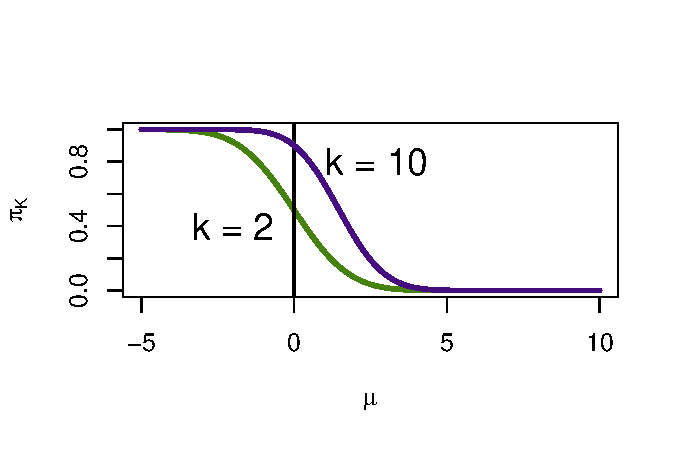
\includegraphics[scale = 0.5, clip=true, trim=0 0.2in 0 0.5in]{../arxiv_info_theory/illus_piK_flat.pdf}} &
\multirow{5}{*}{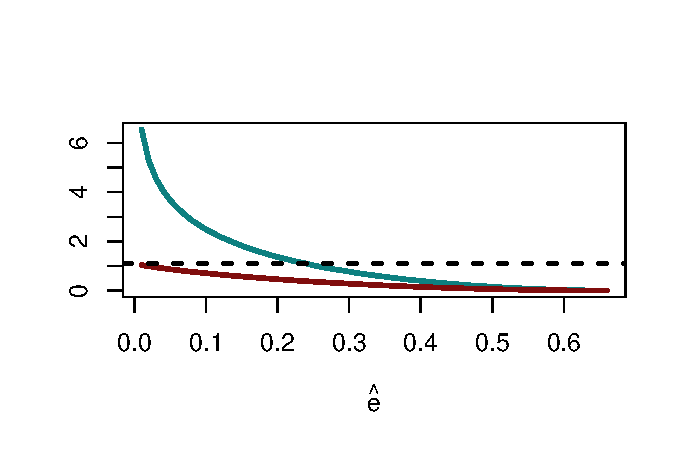
\includegraphics[scale = 0.5, clip=true, trim=0 0.2in 0.4in 0.5in]{../arxiv_info_theory/ihat_comp.pdf}} & & \\
& & & \\
& & \crule[color3]{0.2cm}{0.2cm} & $\hat{I}_{HD}$\\
& & \crule[color1]{0.2cm}{0.2cm} & $\hat{I}_{Fano}$\\
& & & \\
& & & \\
& & & \\
& & & 
\end{tabular}
\caption{Left: The function $pi_k(\mu)$ for $k = \{2, 10\}$.
Right: $\hat{I}_{HD}$ with $\hat{I}_{Fano}$ as functions of $\hat{e}_{gen}$, for $k = 3$.
While $\hat{I}_{Fano}$ is bounded from above by $\log(k)$ (dotted line), $\hat{I}_{HD}$ is unbounded.
[NOTE: 1-$\pi_k$ is displayed, rather than $\pi_k$. Figure to be fixed!]}
\label{fig:pi}
\end{figure}

The estimator we propose is
\begin{equation}\label{eq:hat_i_hd}
\hat{I}_{HD} = \frac{1}{2}(\pi_{k}^{-1}(\text{ABA}_k))^2,
\end{equation}
obtained by inverting the relation \eqref{abepi}, then substituting
an estimate of the identification accuracy $\text{TA}_k$ for the $\text{ABA}_k$.  As such,
our estimator can be directly compared to the $\hat{I}_{Fano}$, since
both are functions of $\text{ABA}_k$ (Figure \ref{fig:pi}.)

\section{Theory}

\subsection{Assumptions}\label{sec:ch5_assumptions}

The theory applies to a high-dimensional limit where $I(X; Y)$ tends to a constant.

\begin{itemize}
\item[A1.] $\lim_{d \to \infty} I(X^{[d]}; Y^{[d]}) = \iota < \infty.$
\item[A2.] There exists a sequence of scaling constants $a_{ij}^{[d]}$
and $b_{ij}^{[d]}$ such that the random vector $(a_{ij}\ell_{ij}^{[d]} +
b_{ij}^{[d]})_{i, j = 1,\hdots, k}$ converges in distribution to a
multivariate normal distribution,
where $\ell_{ij} = \log p(y^{(i)}|x^{(i)})$ for independent $y^{(i)} \sim p(y|x^{(i)})$.
\item[A3.] Define \[
u^{[d]}(x, y) = \log p^{[d]}(x, y) - \log p^{[d]}(x) - \log p^{[d]}(y).
\]
There exists a sequence of scaling constants $a^{[d]}$, $b^{[d]}$ such that
\[
a^{[d]}u^{[d]}(X^{(1)}, Y^{(2)}) + b^{[d]}
\]
converges in distribution to a univariate normal distribution.
\item[A4.] For all $i \neq k$,
\[\lim_{d \to \infty}\Cov[u^{[d]}(X^{(i)}, Y^{(j)}), u^{[d]}(X^{(k)}, Y^{(j)})] = 0.\]
\end{itemize}

Assumptions A1-A4 are satisfied in a variety of natural models.  One
example is a multivariate Gaussian sequence model where $X \sim N(0,
\Sigma_d)$ and $ Y = X + E $ with $ E \sim N(0, \Sigma_e), $ where
$\Sigma_d$ and $\Sigma_e$ are $d \times d$ covariance matrices, and
where $X$ and $E$ are independent.  Then, if $d \Sigma_d$ and
$\Sigma_e$ have limiting spectra $H$ and $G$ respectively, the joint
densities $p(x, y)$ for $d = 1,\hdots, $ satisfy assumptions A1 - A4.
Another example is the multivariate logistic model, which we describe
in section 3.  We further discuss the rationale behind A1-A4 in the
supplement, along with the detailed proof.

\subsection{Limiting universality}

We obtain the universality result in two steps.  First, we link the
average Bayes error to the moments of some statistics $Z_i$.
Secondly, we use Taylor approximation in order to express $I(X; Y)$ in
terms of the moments of $Z_i$.  Connecting these two pieces yields the
formula \eqref{abepi}.

Let us start by rewriting the average Bayes error:
\[
\text{ABA}_k = \Pr[p(Y|X_1) = \max_{j \neq 1} p(Y|X_j)| X = X_1].
\]
Defining the statistic $Z_i = \log p(Y|X_i) - \log p(Y|X_1)$, where $Y
\sim p(y|X_1)$, we obtain $ e_{ABE} = \Pr[\max_{j > 1} Z_i > 0].  $
The key assumption we need is that $Z_2,\hdots, Z_k$ are
asymptotically multivariate normal.  If so, the following lemma allows
us to obtain a formula for the average Bayes accuracy.

\textbf{Lemma 1. }
\emph{
Suppose $(Z_1, Z_2, \hdots, Z_k)$ are jointly multivariate normal, with 
$\E[Z_1 - Z_i]= \alpha$, 
$\Var(Z_1) = \beta \geq 0$, 
$\Cov(Z_1, Z_i) = \gamma$, 
$\Var(Z_i)= \delta$, and $\Cov(Z_i, Z_j) = \epsilon$ for all $i, j = 2, \hdots,
k$, such that $\beta + \epsilon - 2\gamma > 0$.  Then, letting
\[
\mu = \frac{\E[Z_1 - Z_i]}{\sqrt{\frac{1}{2}\Var(Z_i - Z_j)}} = \frac{\alpha}{\sqrt{\delta - \epsilon}},
\]
\[
\nu^2 = \frac{\Cov(Z_1 -Z_i, Z_1 - Z_j)}{\frac{1}{2}\Var(Z_i - Z_j)} = \frac{\beta + \epsilon - 2\gamma}{\delta - \epsilon},
\]
we have
\begin{align*}
\Pr[Z_1 < \max_{i=2}^k Z_i] &= \Pr[W < M_{k-1}]
\\&= 1 - \int \frac{1}{\sqrt{2\pi\nu^2}} e^{-\frac{(w-\mu)^2}{2\nu^2}} \Phi(w)^{k-1} dw,
\end{align*}
where $W \sim N(\mu, \nu^2)$ and $M_{k-1}$ is the maximum of $k-1$
independent standard normal variates, which are independent of $W$.
}

\emph{Remark.}
To see why the assumption that $Z_2,\hdots, Z_k$ are multivariate
normal might be justified, suppose that $X$ and $Y$ have the same
dimensionality $d$, and that joint density factorizes as
\[
p(x^{(j)}, y) = \prod_{i=1}^d p_i(x^{(j)}_i, y_i)
\]
where $x_i^{(j)}, y_i$ are the $i$th scalar components of the vectors $x^{(j)}$ and $y$.
Then,
\[
Z_i = \sum_{m=1}^d \log p_m(y_m | x^{(i)}_m) - \log p_m(y_m | x^{(m)}_1)
\]
where $x_{i, j}$ is the $i$th component of $x_j$.  The $d$ terms $\log
p_m(y_m | x_{m, i}) - \log p_m(y_m | x_{m, 1})$ are independent across
the indices $m$, but dependent between the $i = 1,\hdots, k$.
Therefore, the multivariate central limit theorem can be applied to
conclude that the vector $(Z_2,\hdots, Z_k)$ can be scaled to converge
to a multivariate normal distribution.  While the componentwise
independence condition is not a realistic assumption, the key property
of multivariate normality of $(Z_2,\hdots, Z_k)$ holds under more
general conditions, and appears reasonable in practice.

\textbf{Proof.}
We can construct independent normal variates $G_1$, $G_2,\hdots, G_k$
such that
\[
G_1 \sim N(0, \beta + \epsilon - 2 \gamma)
\]
\[
G_i \sim N(0, \delta - \epsilon)\text{ for }i > 1
\]
such that
\[
Z_1 - Z_i = \alpha + G_1 + G_i \text{ for }i > 1.
\]
Hence
\begin{align*}
\Pr[Z_1 < \max_{i=2}^k Z_i] &= \Pr[\min_{i > 1} Z_1 - Z_i < 0].
\\&= \Pr[\min_{i=2}^{k} G_1 + G_i + \alpha < 0]
\\&= \Pr[\min_{i=2}^{k} G_i < -\alpha - G_1]
\\&= \Pr[\min_{i=2}^{k} \frac{G_i}{\sqrt{\delta - \epsilon}} < -\frac{\alpha - G_1}{\sqrt{\delta - \epsilon}}].
\end{align*}
Since $\frac{G_i}{\sqrt{\delta - \epsilon}}$ are iid standard normal variates, and since
$-\frac{\alpha - G_1}{\sqrt{\delta - \epsilon}} \sim N(\mu,\nu^2)$ for $\mu$ and $\nu^2$ given in the statement of the Lemma, the proof is completed via a straightforward computation.  $\Box$



It remains to link the moments of $Z_i$ to $I(X;Y)$.  This is accomplished by approximating the logarithmic term by the Taylor expansion
\[
\log \frac{p(x, y)}{p(x) p(y)} \approx \frac{p(x, y) - p(x) p(y)}{p(x) p(y)} - \left(\frac{p(x, y) - p(x) p(y)}{p(x) p(y)}\right)^2 + \hdots.
\]
A number of assumptions are needed to ensure that needed
approximations are sufficiently accurate; and additionally, in order
to apply the central limit theorem, we need to consider a
\emph{limiting sequence} of problems with increasing dimensionality.
We now state the theorem.

\textbf{Theorem 1.} \emph{Let $p^{[d]}(x, y)$ be a sequence of joint densities
for $d = 1,2,\hdots$.  Further assume that
\begin{itemize}
\item[A1.] $\lim_{d \to \infty} I(X^{[d]}; Y^{[d]}) = \iota < \infty.$
\item[A2.] There exists a sequence of scaling constants $a_{ij}^{[d]}$
and $b_{ij}^{[d]}$ such that the random vector $(a_{ij}\ell_{ij}^{[d]} +
b_{ij}^{[d]})_{i, j = 1,\hdots, k}$ converges in distribution to a
multivariate normal distribution,
where $\ell_{ij} = \log p(y^{(i)}|x^{(i)})$ for independent $y^{(i)} \sim p(y|x^{(i)})$.
\item[A3.] Define \[
u^{[d]}(x, y) = \log p^{[d]}(x, y) - \log p^{[d]}(x) - \log p^{[d]}(y).
\]
There exists a sequence of scaling constants $a^{[d]}$, $b^{[d]}$ such that
\[
a^{[d]}u^{[d]}(X^{(1)}, Y^{(2)}) + b^{[d]}
\]
converges in distribution to a univariate normal distribution.
\item[A4.] For all $i \neq k$,
\[\lim_{d \to \infty}\Cov[u^{[d]}(X^{(i)}, Y^{(j)}), u^{[d]}(X^{(k)}, Y^{(j)})] = 0.\]
\end{itemize}
Then for $\text{ABA}_k$ as defined above, we have
\[
\lim_{d \to \infty} \text{ABA}_k = \pi_k(\sqrt{2 \iota})
\]
where
\[
\pi_k(c) = \int_{\mathbb{R}} \phi(z - c)  \Phi(z)^{k-1} dz
\]
where $\phi$ and $\Phi$ are the standard normal density function and
cumulative distribution function, respectively.}


\textbf{Proof.}

For $i = 2,\hdots, k$, define
\[
Z_i = \log p(Y^{(1)}|X^{(i)}) - \log p(Y^{(1)}|X^{(1)}).
\]
Then, we claim that $\vec{Z} = (Z_2,\hdots, Z_k)$ converges in distribution to
\[
\vec{Z} \sim N\left(-2\iota, 
\begin{bmatrix}
4\iota & 2\iota & \cdots & 2\iota\\
2\iota & 4\iota & \cdots & 2\iota\\
\vdots & \vdots & \ddots & \vdots\\
2\iota & 2\iota & \cdots & 4\iota
\end{bmatrix}
\right).
\]
Combining the claim with the lemma (stated below this proof) yields the
desired result.

To prove the claim, it suffices to derive the limiting moments
\[\E[Z_i] \to -2\iota,\]
\[\Var[Z_i] \to 4\iota,\]
\[\Cov[Z_i, Z_j] \to 2\iota,\]
for $i \neq j$,
since then assumption A2 implies the existence of a multivariate normal
limiting distribution with the given moments.

Before deriving the limiting moments, note the following identities.
Let $X' = X^{(2)}$ and $Y = Y^{(1)}$.
\[
\E[e^{u(X', Y)}] = \int p(x) p(y) e^{u(x, y)} dx dy = \int p(x, y) dx dy = 1.
\]
Therefore, from assumption A3 and the formula for gaussian exponential
moments, we have
\[
\lim_{d \to \infty} \E[u(X', Y)]-\frac{1}{2}\Var[u(X', Y)] = 0.
\]
Let $\sigma^2 = \lim_{d \to \infty} \Var[u(X', Y)]$.
Meanwhile, by applying assumption A2,
\begin{align*}
\lim_{d \to \infty} I(X; Y) &= \lim_{d \to \infty} \int p(x, y) u(x, y) dx dy 
= \lim_{d \to \infty} \int p(x) p(y) e^{u(x, y)} u(x, y) dx dy
\\&= \lim_{d \to \infty}  \E[e^{u(X, Y')}u(X, Y')]
\\&= \int_{\mathbb{R}} e^z z \frac{1}{\sqrt{2\pi \sigma^2}} 
e^{-\frac{(z + \sigma^2/2)^2}{2\sigma^2}} \text{ (applying A2)}
\\&= \int_{\mathbb{R}} z \frac{1}{\sqrt{2\pi \sigma^2}} 
e^{-\frac{(z - \sigma^2/2)^2}{2\sigma^2}}
\\&= \frac{1}{2}\sigma^2.
\end{align*}
Therefore,
\[
\sigma^2 = 2\iota,
\]
and
\[
\lim_{d \to \infty} \E[u(X', Y)] = -\iota.
\]
Once again by applying A2, we get
\begin{align*}
\lim_{d \to \infty} \Var[u(X, Y)] 
&= \lim_{d \to \infty} \int (u(x, y) - \iota)^2 p(x, y) dx dy
\\&= \lim_{d \to \infty} \int (u(x, y) - \iota)^2 e^{u(x, y)} p(x) p(y) dx dy
\\&= \lim_{d \to \infty} \E[(u(X', Y) - \iota)^2 e^{u(X', Y)}] 
\\&= \int (z - \iota)^2 e^z \frac{1}{\sqrt{4\pi\iota}} e^{-\frac{(z+\iota)^2}{4\iota}} dz \text{ (applying A2)}
\\&= \int (z - \iota)^2 \frac{1}{\sqrt{4\pi\iota}} e^{-\frac{(z-\iota)^2}{4\iota}} dz
\\&= 2\iota.
\end{align*}


We now proceed to derive the limiting moments.
We have
\begin{align*}
\lim_{d \to \infty} \E[Z] 
&= \lim_{d \to \infty} \E[ \log p(Y|X') - \log p(Y|X)]
\\&= \lim_{d \to \infty} \E[ u(X', Y) - u(X, Y) ] = -2\iota.
\end{align*}
Also,
\begin{align*}
\lim_{d \to \infty} \Var[Z]
 &= \lim_{d \to \infty} \Var[ u(X', Y) - u(X, Y) ]
\\&= \lim_{d \to \infty} \Var[ u(X', Y)] +\Var[ u(X, Y) ]\text{ (using assumption A4) }
\\&= 4\iota,
\end{align*}
and similarly
\begin{align*}
\lim_{d \to \infty} \Cov[Z_i, Z_j]
&= \lim_{d \to \infty} \Var[ u(X, Y)]\text{ (using assumption A4) }
\\&= 2\iota.
\end{align*}
This concludes the proof. $\Box$.

\section{Examples}

We demonstrate the application of our proposed estimators,
$\hat{I}_{Ident}$, which was introduced in the previous chapter, and
the estimator $\hat{I}_{HD}$ based on high-dimensional asymptotics, as
defined in \eqref{eq:hat_i_hd}.

We compare our methods to a number of existing methods for mutual
information.  For any $k$-class classification task, define the $k
\times k$ \emph{confusion matrix} $M$ as the matrix whose $i, j$
counts how many times a output in the $i$th class was classified to
the $j$th class.

The estimator $\hat{I}_{Fano}$ is based on Fano's inequality, which reads
\[
H(Z|Y) \leq H(1-\text{BA}) + (1-\text{BA}) \log ||\mathcal{Z}| - 1|
\]
where $\text{BA}$ is Bayes accuracy, and $H(e)$ is the entropy of a
Bernoulli random variable with probability $e$.  Replacing $H(Z|Y)$
with $H(X|Y)$ and replacing $\text{BA}$ with the test accuracy $\text{TA}$,
we get the estimator
\[
\hat{I}_{Fano} = log(K) - (1-\text{TA}) log(K-1) + (1-\text{TA}) log(1-\text{TA}) + \text{TA} log(\text{TA}).
\]
Meanwhile, the confusion matrix estimator computes
\[
\hat{I}_{CM} = \frac{1}{k^2} \sum_{i=1}^k \sum_{j=1}^k \log \frac{M_{ij}}{r/k},
\]
which is the empirical mutual information of the discrete joint
distribution $(Z, f(Y))$.

The estimator $\hat{I}_0$ is the so-called `naive' estimate of mutual information, based on the identity
\[
I(X;Y) = H(Y) - H(Y|X).
\]
Given any nonparametric estimator of entropy $\hat{H}$, we obtain
\[
\hat{I}_0 = \hat{H}(Y) - \sum_{i=1}^k \hat{H}(Y|X^{(i)}).
\]
We use the polynomial-based entropy estimator introduced by
\cite{jiao2015minimax} as the estimator of entropy.  

It is known that $\hat{I}_0$ tends to underestimate the mutual
information.  Therefore, Gastpar et al. introduced the anthropic
correction estimator $\hat{I}_\alpha$ which adds a bias-correction
term \footnote{However, without a principled approach to choose the
  parameter $\alpha \in (0,1]$, $\hat{I}_\alpha$ could still vastly
underestimate or overestimate the mutual information.}to $\hat{I}_0$.

\subsection{Simulation}

We compare the estimators $\hat{I}_{CM}$, $\hat{I}_{Fano}$,
$\hat{I}_{HD}$ with a nonparametric estimator $\hat{I}_\alpha$
(\cite{Gastpar2009}) in the following simulation, and the correctly
specified parametric estimator $\hat{I}_{MLE}$.  We generate data
according to a multiple-response logistic regression model, where $ X
\sim N(0, I_p) $, and $Y$ is a binary vector with conditional
distribution
\[
Y_i|X = x \sim \text{Bernoulli}(x^T B_i)
\]
where $B$ is a $p \times q$ matrix.  We generate training data with
$r$ responses per stimulus $X^{(i)}$.  One application of this model
might be modeling neural spike count data $Y$ arising in response to
environmental stimuli $X$ (\cite{banerjee2012parametric}).  We choose
the naive Bayes for the classifier $\mathcal{F}$: it is consistent for
estimating the Bayes rule.

\begin{figure}
\centering
\begin{tabular}{cc}
a & b\\
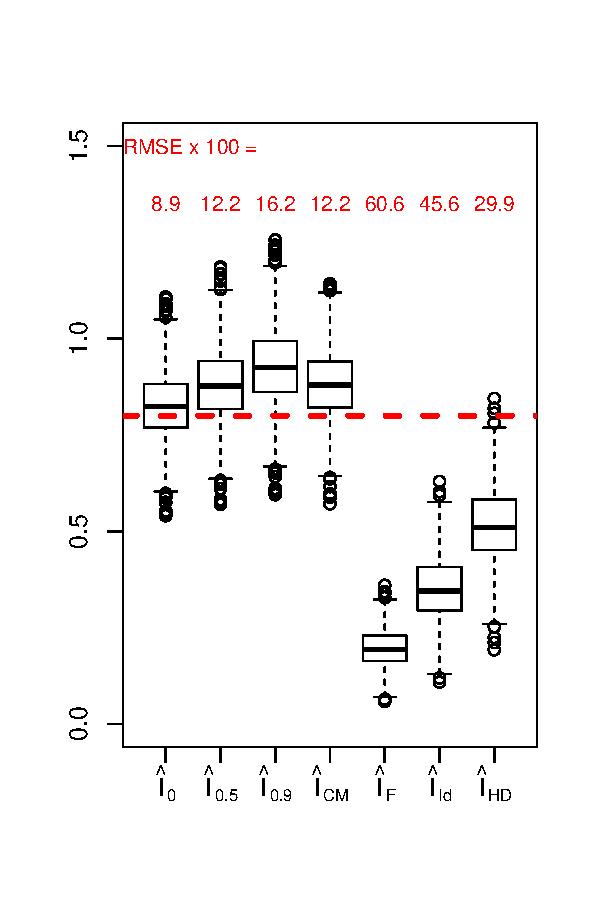
\includegraphics[scale = 0.5]{../../info_theory_sims/fig1_with_Id.pdf} &
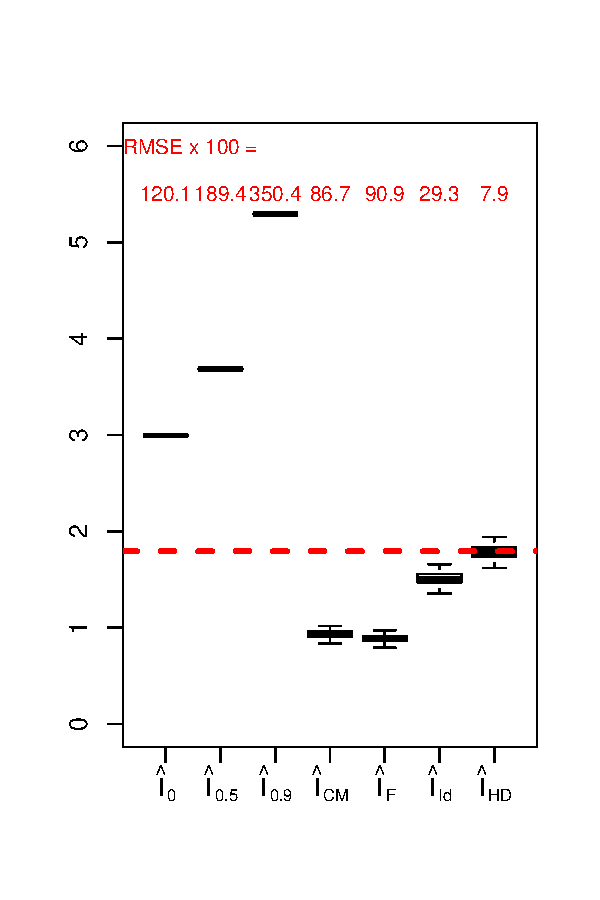
\includegraphics[scale = 0.5]{../../info_theory_sims/fig2_with_Id.pdf}
\end{tabular}
\caption{Simulation for inferring mutual information in a gaussian random classification model}
\label{fig:gaussian_sim}
\end{figure}

Figure \ref{fig:gaussian_sim} displays the simulation results for two
cases: 
\begin{itemize}
\item[(a).] A low-dimensional example with $\{p = 3$, $q = 3$, $B = \frac{4}{\sqrt{3}} I_3$, $K = 20$, $r = 40\}$
\item[(b).] A high-dimenaional example with $\{p = 50$, $q = 50$, $B = \frac{4}{\sqrt{50}} I_{50}$, $K = 20$, $r = 8000\}$
\end{itemize}
We see that in the low-dimensional example, the na\"{i}ve estimator
$\hat{I}_0$ achieves the best performance, with both of our proposed
estimators $\hat{I}_{Ident}$ and $\hat{I}_{HD}$ biased downwards.
However, in the high-dimensional example, which approximately
satisfies the assumptions of our high-dimensional theory, we see that
all estimators of mutual information become highly concentrated.
Therefore, it is the amount of bias in the estimator that mainly
determines estimation performance.  We see heavy bias in estimators
except for $\hat{I}_{HD}$, which is to be expected since the
nonparametric estimators $\hat{I}_\alpha$ scale poorly in high
dimensions, while $\hat{I}_{CM}, \hat{I}_{Fano}$ and $\hat{I}_{Ident}$
are based on lower bounds and therefore should have a downward bias.

\subsection{Real data example}\label{sec:real_data}

\cite{Kay2008a} employed a randomized stimuli design in their 2008 paper,
``Identifying Natural Images from Human Brain Activity.''  The
experiment was designed in order to investigate how visual information
from natural images is encoded in the V1 through V3 brain regions.
The stimulus space, $\mathcal{X}$, consists of $128 \times 128$-pixel
grayscale photographs.  The response data consists of BOLD response in
regions V1, V2, and V3 from a single subject.  The raw time series were
processed to yield a single averaged response vector $y^{(i)}$ for each
stimulus $x^{(i)}$, for $i = 1,\hdots, 1870$.
The dimensionality of $y^{(i)}$ varies depending on which regions of interest
we are discussing, and whether we consider a subset of the voxels in those regions.
Let $v$ denote the dimensionality (number of voxels) of $y$.

Let $x^{(i)}$ denote the native $128 \times 128$-pixel representation
of the image (i.e. a $16384$-dimensional vector with entries between 0
and 1.)  One of the goals of the Kay et al. paper is to evaluate
competing encoding models.  In the context of the study,
an \emph{encoding model} is a vector-valued function from the stimulus
to a $p$-dimensional space,
\[
\vec{g}(x) = (g_1(x),\hdots, g_{p}(x)).
\]
One of the encoding models studied by Kay et al. is the Gabor wavelet pyramid,
$\vec{g}_{Gabor}$, with $p = 10921$.
Using a \emph{training} subset of the stimulus-response pairs $(x_i, y_i)$, $i = 1,\hdots, 1750$,
Kay et al. fit a regularized linear model
\[
y^{(i)} \approx B^T \vec{g}(x^{(i)})
\]
where $B$ is a $10921 \times v$-dimensional matrix, which is to be fit
to the data.  Then they computed the identification accuracy for $k$
(number of stimulus classes) ranging from 2 to 1000.

Using the Kay et al. data, we sort voxels in V1 according to estimated
signal-to-noise ratio (\cite{benjamini2013shuffle}).  Then, using
cross-validated elastic net on the top $p = \{100, 200, 300, 400,
500\}$ voxels, we compute the identification accuracy for $k =
\{20,\hdots, 240\}$ classes.  The test identification accuracy was
used to estimate mutual information using both $\hat{I}_{Ident}$ and
$\hat{I}_{HD}$.  Due to the dimensionality of the data, we expected
$\hat{I}_{HD}$ to yield more accurate estimates of mutual information.

The estimated mutual information using $k = 240$ is displayed in
Figure \ref{fig:n_voxels_vs_mi}.  Both estimators indicate a large
jump in the mutual information when going from 100 to 200 voxels,
almost no increase from 200 to 400, then a slight increase in
information from 400 to 500.  The two estimators $\hat{I}_{Ident}$ and
$\hat{I}_{HD}$ differ significantly for all numbers of voxels. We see
from this that it is important to choose the estimator which is best
suited for the application: if the high-dimensional assumption can be
justified, $\hat{I}_{HD}$ can yield a much better estimate; but if not
justified, then it could be a significant overestimate of the mutual
information, and it would be preferable to use $\hat{I}_{Ident}$.

\begin{figure}
\centering
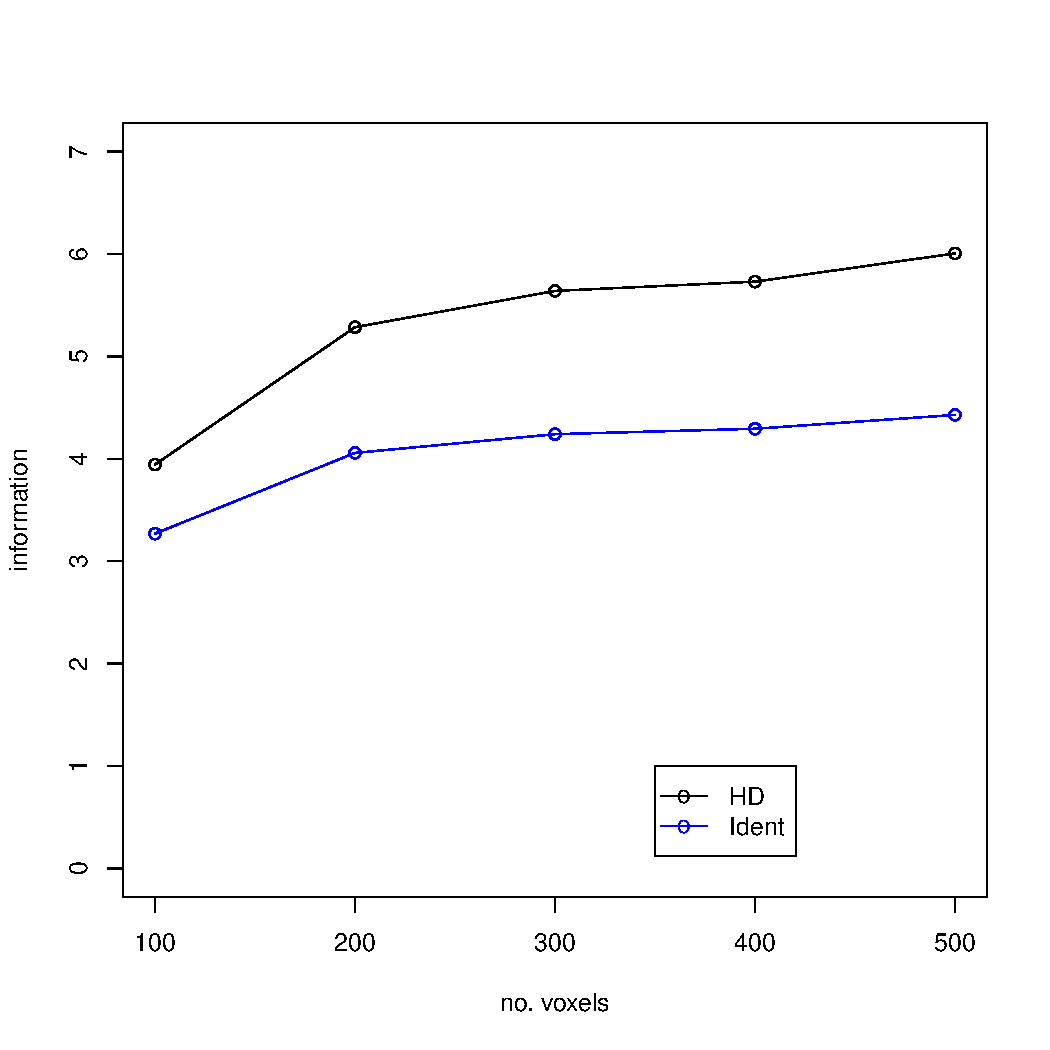
\includegraphics[scale = 0.5]{../../Yuval/info_infer.pdf}
\caption{Estimated mutual information for different subsets of V1 voxels}
\label{fig:n_voxels_vs_mi}
\end{figure}

Next, let us examine the sensitivity of the point estimates to the
choice of the tuning parameter $k$.  Figure \ref{fig:dependence_k}
shows how the estimates displayed in the previous figure depend on the
choice of $k$.  For all numbers of voxels, we see that $k$ does have
an appreciable affect on the resulting estimate of mutual information.
This is predicted from the theory for $\hat{I}_{Ident}$, but under the
high-dimensionality assumptions $\hat{I}_{HD}$ should not be
significantly depend on $k$.  Therefore, the sensitivity of
$\hat{I}_{HD}$ we see, especially for the 500-voxel case, indicates a
detectable violation of the asymptotic assumptions.

Given such evidence for violation of assumptions, the conservative
approach would be to abandon $\hat{I}_{HD}$ in this situation and
choose $\hat{I}_{Ident}$ as the estimator. Since $\hat{I}_{Ident}$ is
an underestimate for all $k$, one should choose the $k$ which
maximizes the estimated mutual information.  However, even then, as we
see from the earlier simulation, we can expect $\hat{I}_{Ident}$ to
significantly underestimate the true mutual information.

\begin{figure}
\centering
\begin{tabular}{cc}
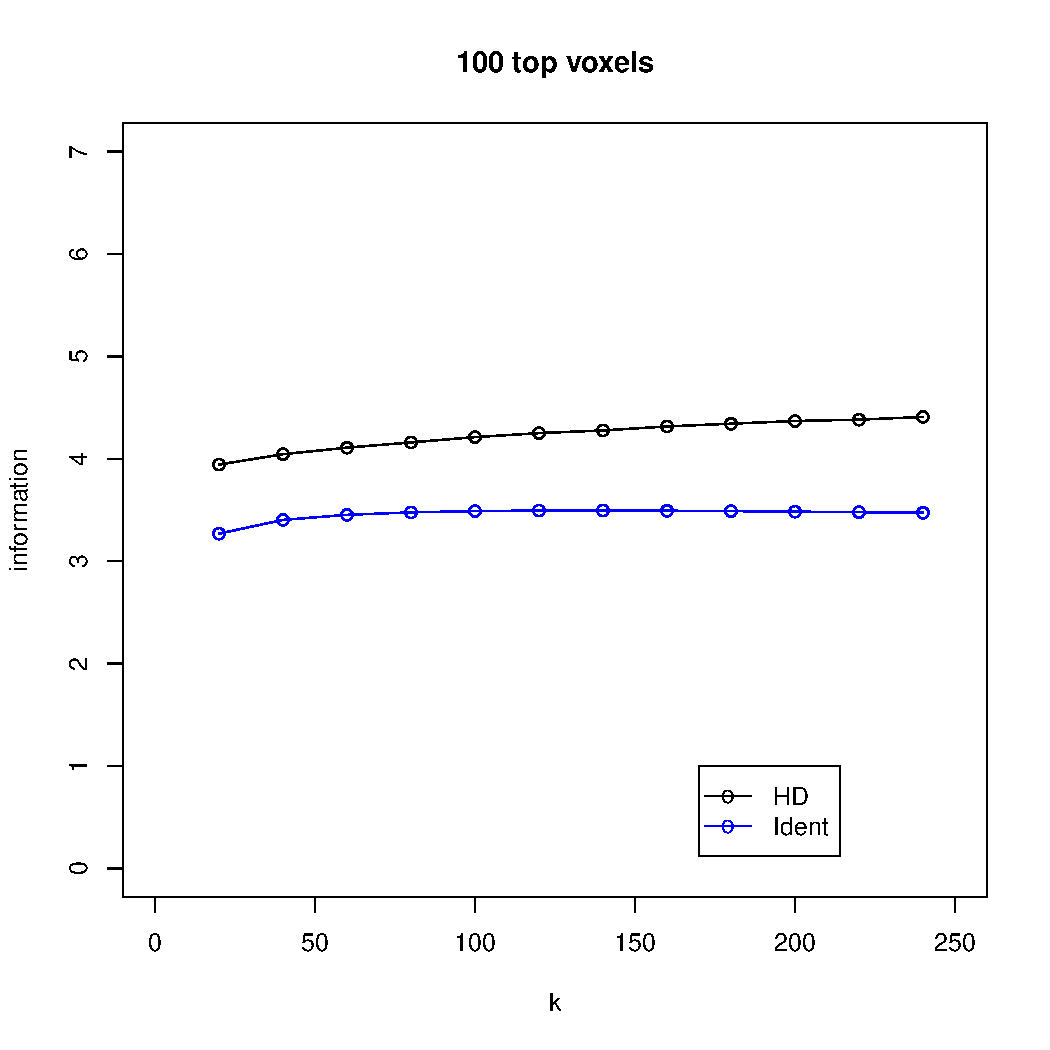
\includegraphics[scale = 0.4]{../../Yuval/ident_infer1.pdf} &
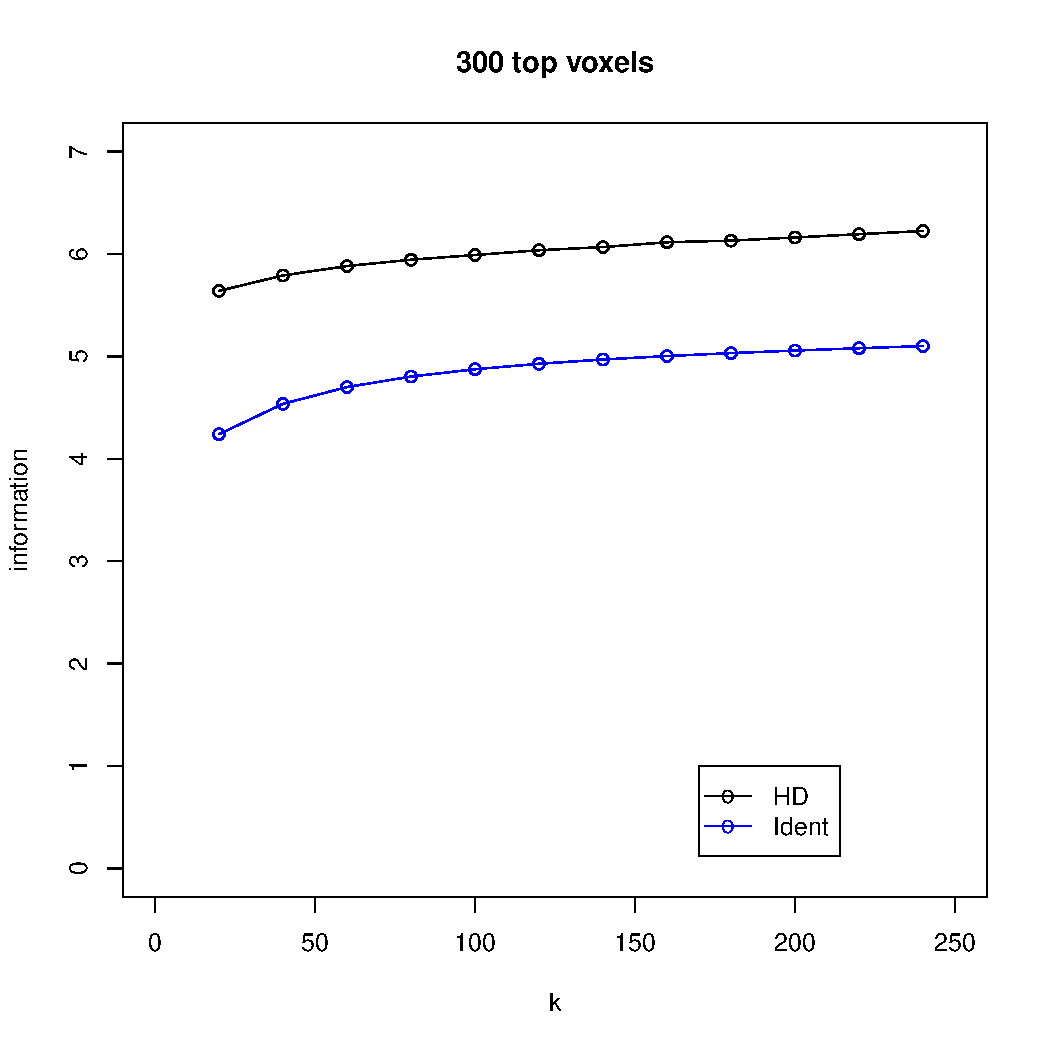
\includegraphics[scale = 0.4]{../../Yuval/ident_infer3.pdf} \\
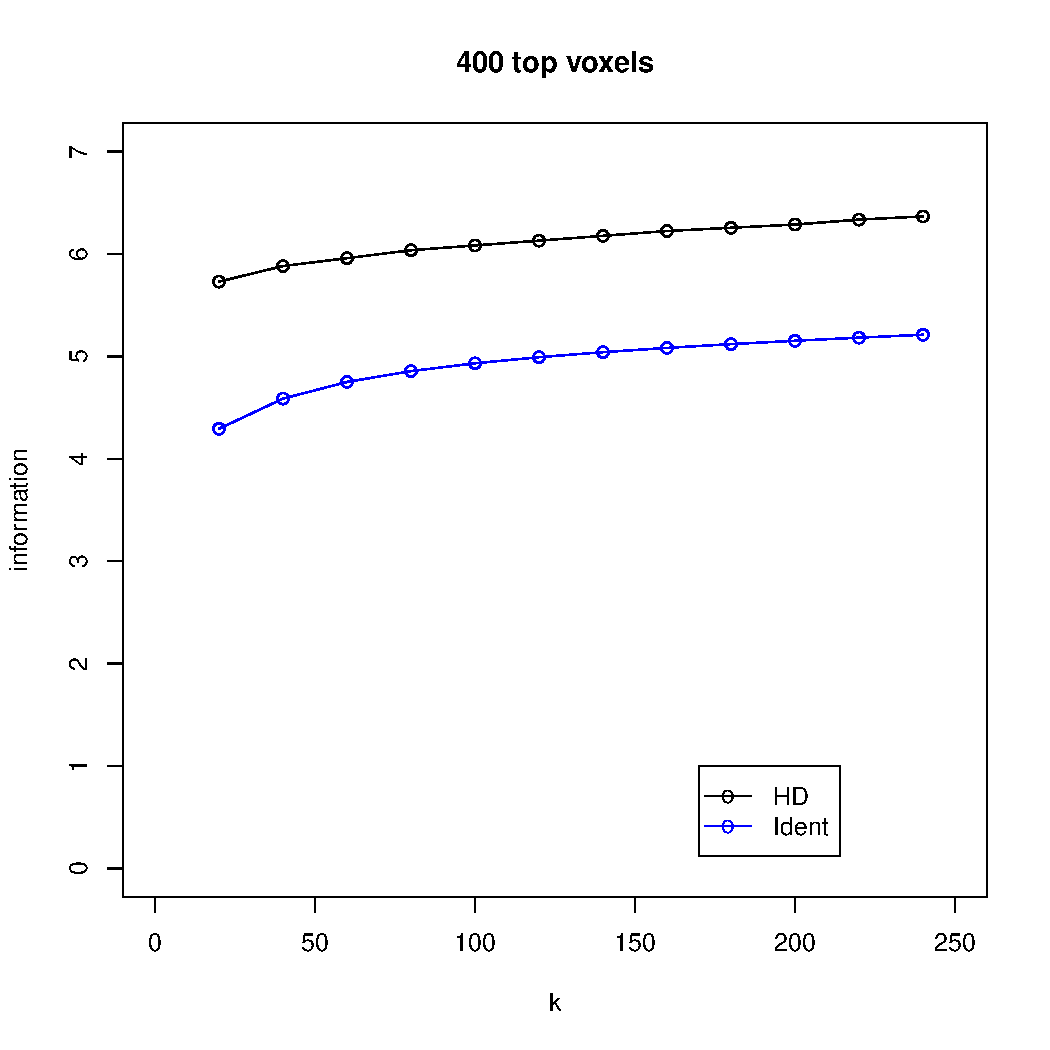
\includegraphics[scale = 0.4]{../../Yuval/ident_infer4.pdf} &
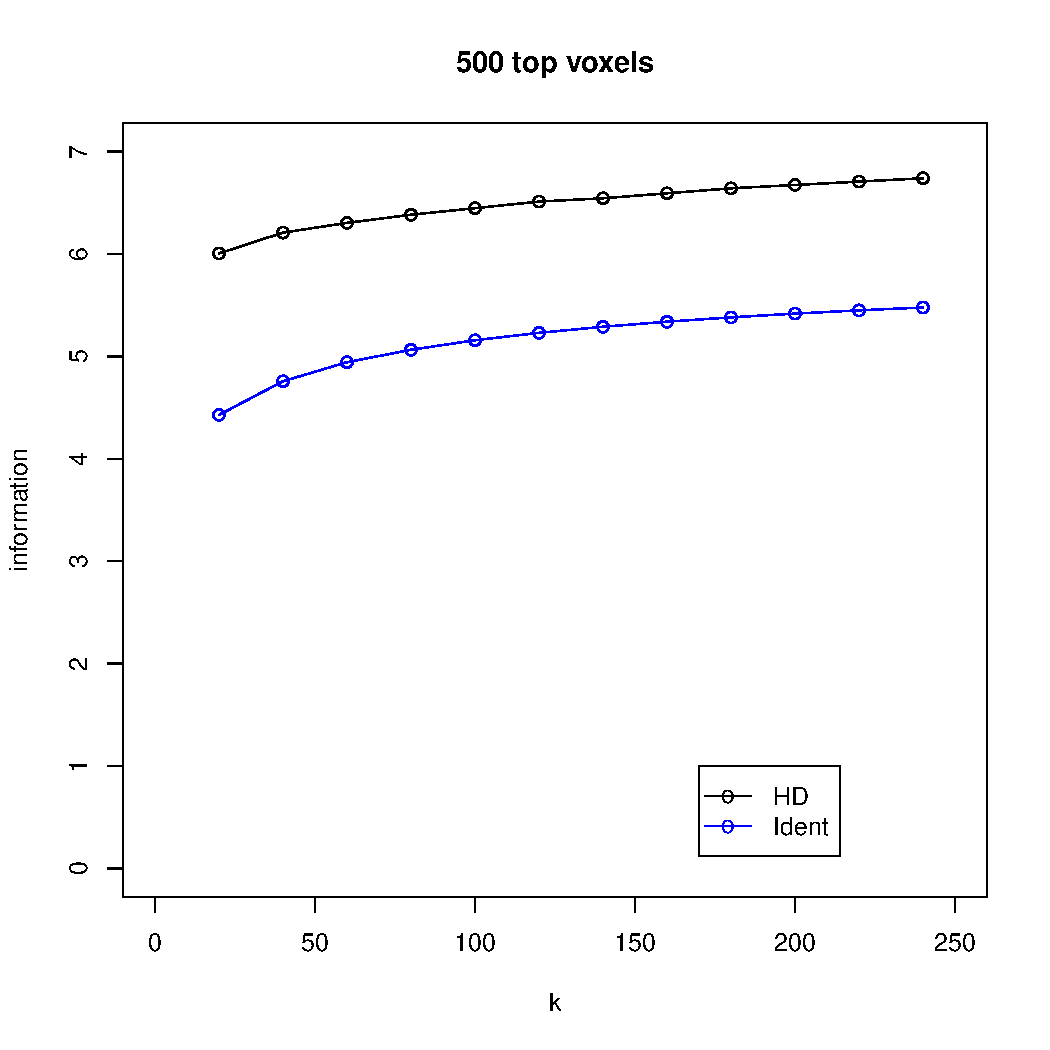
\includegraphics[scale = 0.4]{../../Yuval/ident_infer5.pdf}
\end{tabular}
\caption{Dependence of estimated mutual information on $k$}
\label{fig:dependence_k}
\end{figure}


 

%----------------------------------------------------------------------------------------
%	THESIS CONTENT - APPENDICES
%----------------------------------------------------------------------------------------

\appendix % Cue to tell LaTeX that the following "chapters" are Appendices

% Include the appendices of the thesis as separate files from the Appendices folder
% Uncomment the lines as you write the Appendices

% Appendix A

\chapter{Appendix for Chapter 1} % Main appendix title

\label{AppendixA} % For referencing this appendix elsewhere, use \ref{AppendixA}

\section{Proofs}


%% Appendix B

\chapter{Frequently Asked Questions} % Main appendix title

\label{AppendixB} % For referencing this appendix elsewhere, use \ref{AppendixA}

\section{How do I change the colors of links?}

The color of links can be changed to your liking using:

{\small\verb!\hypersetup{urlcolor=red}!}, or

{\small\verb!\hypersetup{citecolor=green}!}, or

{\small\verb!\hypersetup{allcolor=blue}!}.

\noindent If you want to completely hide the links, you can use:

{\small\verb!\hypersetup{allcolors=.}!}, or even better: 

{\small\verb!\hypersetup{hidelinks}!}.

\noindent If you want to have obvious links in the PDF but not the printed text, use:

{\small\verb!\hypersetup{colorlinks=false}!}.

%% Appendix C

\chapter{Appendix for Chapter 3} % Main appendix title

\label{AppendixC} % For referencing this appendix elsewhere, use \ref{AppendixA}

\section{Proofs}

\begin{lemma}\label{lemma:U_function}
Suppose $\pi$, $\{F_y\}_{y \in \mathcal{Y}}$ and marginal classifier
$\mathcal{F}$ satisfy the tie-breaking condition.  Take $x \in \mathcal{X}$.  Defining
$U_{y,\hat{F}_y}(x)$ as in \eqref{eq:U_function}, and defining the
random variable $U$ by
\[U = U_{Y, \hat{F}_Y}(x)\]
for $Y \sim \pi$, $\hat{F}_Y \sim \Pi_{Y, r}$,
the distribution of $U$ is uniform on $[0,1]$, i.e.
\[
\Pr[U \leq u] = \text{max}\{u, 1\}.
\]
\end{lemma}

\textbf{Proof of Lemma A.1.}

Define the variable $Z = \mathcal{M}(\hat{F}_Y)(x)$ for $Y \sim \pi$.
By the tie-breaking condition, $Z$ has a continuous density on $[0,1]$.
Consider the survivor function of $Z$, $g(z) = \Pr[Z \geq z]$.  From
the definition \eqref{eq:U_function}, we see that 
\[
U = g(\mathcal{M}(\hat{F}_Y)(x)) = g(Z).
\]
Now note that the survivor function of any continuous random variable,
when applied to itself, is uniformly distributed.
$\Box$


%----------------------------------------------------------------------------------------
%	BIBLIOGRAPHY
%----------------------------------------------------------------------------------------

\printbibliography[heading=bibintoc]

%----------------------------------------------------------------------------------------

\end{document}  
